\def\PageLayout{single-no-print}
\def\DocLanguage{en}
\def\PackagesIncludeTikz{yes}
\def\PackagesIncludeBib{yes}

%%% Please fill in basic information on your thesis, which will be automatically
%%% inserted at the right places. You need to replace ... by real data.

% Type of your thesis:
%	"bc" for Bachelor's
%	"mgr" for Master's
%	"phd" for PhD
%	"rig" for rigorosum
% "sem" for semestral
\def\ThesisType{bc}


\def\ThesisTitle{Surveillance FMCW Radar}

\def\ThesisTitleShort{Surveillance FMCW Radar}

\def\ThesisAuthor{Havránek Kryštof}

\def\MontSubmitted{TODO}

\def\YearSubmitted{2024}

\def\Institution{Czech Technical University in Prague}

\def\Faculty{Faculty of Electrical Engineering}

\def\DepartmentType{Department}

\def\Department{Department of Electromagnetic Field}

\def\Supervisor{Ing. Viktor Adler, Ph.D}

\def\SupervisorsDepartment{Department of Electromagnetic Field}

\def\StudyProgramme{Elektronika a komunikace}

\def\Dedication{%
Dedication.
}

\def\Abstract{%
	TODO
}

% 3 to 5 keywords (recommended) separated by \sep
% Keywords are useful for indexing and searching for the theses by topic.
\def\ThesisKeywords{%
	TODO
}

% If any of your metadata strings contains TeX macros, you need to provide
% a plain-text version for use in XMP metadata embedded in the output PDF file.
% If you are not sure, check the generated thesis.xmpdata file.
\def\AuthorXMP{\ThesisAuthor}
\def\TitleXMP{\ThesisTitle}
\def\KeywordsXMP{\ThesisKeywords}
\def\AbstractXMP{\Abstract}

% If your abstracts are long and do not fit in the infopage, you can make the
% fonts a bit smaller by this setting. (Also, you should try to compress your abstract more.)
\def\InfoPageFont{}
%\def\InfoPageFont{\small}  % uncomment to decrease font size

% If you are studing in a Czech programme, you also need to provide metadata in Czech:
% (in English programmes, this is not used anywhere)

\def\ThesisTitleCS{Přehledový FMCW radar}
\def\DepartmentCS{Katedra elektromagnetického pole}
\def\DepartmentTypeCS{Katedra}
\def\SupervisorsDepartmentCS{Katedra elektromagnetického pole}
\def\StudyProgrammeCS{Elektronika a komunikace}

\def\ThesisKeywordsCS{%
	TODO
}

\def\AbstractCS{%
	TODO
}


%%% Different page dimensions used on thesis
\def\PageLayoutSingle{single}
\def\PageLayoutSingleNoPrint{single-no-print}
\def\PageLayoutDouble{double}
\def\PageLayoutDoubleNoPrint{double-no-print}



%% Single page print
\ifx\PageLayout\PageLayoutSingle
\documentclass[a4paper,oneside,12pt]{report}
\setlength\textwidth{145mm}
\setlength\textheight{251mm}
\setlength\oddsidemargin{15mm}
\setlength\evensidemargin{15mm}
\setlength\topmargin{-0.4in}
\setlength\headsep{10mm}
\setlength\headheight{0mm}
\let\openright=\clearpage
\fi

%% Double page print
\ifx\PageLayout\PageLayoutDouble
% \documentclass[12pt,a4paper,twoside,openright]{report} % chapter will always start on the right side
\documentclass[12pt,a4paper,twoside]{report}
\setlength\textwidth{145mm}
\setlength\textheight{251mm}
\setlength\oddsidemargin{14.2mm}
\setlength\evensidemargin{0mm}
\setlength\topmargin{-0.4in}
\setlength\headsep{10mm}
\setlength\headheight{0mm}
\let\openright=\clearpage
% \let\openright=\cleardoublepage
\fi

%% Double page without space left for binding
\ifx\PageLayout\PageLayoutDoubleNoPrint
% \documentclass[12pt,a4paper,twoside,openright]{report} % chapter will always start on the right side
\documentclass[12pt,a4paper,twoside]{report}
\setlength\textwidth{145mm}
\setlength\textheight{251mm}
\setlength\oddsidemargin{9mm}
\setlength\evensidemargin{9mm}
\setlength\topmargin{-0.4in}
\setlength\headsep{10mm}
\setlength\headheight{0mm}
\let\openright=\clearpage
% \let\openright=\cleardoublepage
\fi

%% Single page without space left for binding
\ifx\PageLayout\PageLayoutSingleNoPrint
\documentclass[12pt,a4paper]{report}
\setlength\textwidth{145mm}
\setlength\textheight{251mm}
\setlength\oddsidemargin{9mm}
\setlength\evensidemargin{9mm}
\setlength\topmargin{-0.4in}
\setlength\headsep{10mm}
\setlength\headheight{0mm}
\let\openright=\clearpage

\fi




\def\LangCS{cs}
\def\LangEN{en}
\def\ConfirmExpr{yes}




%%% TiKz
% Memoize package needs to be loaded as soon as possible, in beamer even before document declaration
\ifx\PackagesIncludeTikz\ConfirmExpr
	\usepackage{memoize}
	\usepackage{collargs}
	\usepackage{tikz}
	\usepackage{tikz-cd}
	\usepackage{circuitikz}
	\mmzset{memo dir=memoize}
	\mmzset{auto={circuitikz}{memoize}}
	\mmzset{auto={tikzcdi}{memoize, verbatim}}
	\mmzset{auto={tikzpicture}{memoize, verbatim}}

	\usetikzlibrary{calc}
	\usetikzlibrary{fadings}
	\usetikzlibrary{shapes.geometric, arrows, positioning}

	\tikzstyle{layerheader} = [rectangle, minimum width=3cm, minimum height=1cm, text centered, draw=black, fill=gray!30]
	\tikzstyle{startstop} = [ellipse, minimum width=3cm, minimum height=1cm, text centered, draw=black, fill=red!30]
	\tikzstyle{process} = [rectangle, minimum width=3cm, minimum height=1cm, text centered, draw=black, fill=blue!20]
	\tikzstyle{decision} = [diamond, minimum width=2.5cm, minimum height=1cm, text centered, draw=black, fill=green!20]
	\tikzstyle{arrow} = [thick,->,>=stealth]
\fi




\ifx\DocLanguage\LangCS
	\usepackage[czech]{babel}
	\babelprovide[transforms = oneletter.nobreak]{czech} % non break on single letter words in czech
\else
	\usepackage[english]{babel}
\fi


\usepackage[T1]{fontenc}
\usepackage[utf8]{inputenc}
\usepackage{lmodern,textcomp}

\usepackage[a-2u]{pdfx}         % adding metadata to pdf with .xmpdata file
\usepackage{graphicx}						% inserting pictures
\usepackage{caption}						%	captions of figures
\usepackage{subcaption} 				% multiple figures in one figure environment
\usepackage{hyperref} 					% handling of hypertext
\usepackage{tabularx}           % table environment
\usepackage{xcolor,colortbl}    % more options for colors
\usepackage{textpos}            % more precise control over positioning of elements
\usepackage{longtable}          % longtable environment to enable multipage tables
\usepackage{fancyhdr}						% custom header and footer
\usepackage{xurl}								% extension to url handeling, allows linebreaks in urls and more special characters
\usepackage{enumitem}           % more options for labeling lists
\usepackage{multicol}           % simplest environment to achieve multiple columns

%%% Math packages
\usepackage{pgfplots}           % graphs
\usepackage{amsmath}						% extension for math
\usepackage{amsthm}							% environment for lemmas, proofs, theorems, etc.
\usepackage{amssymb} 						% math symbols
\usepackage{mathrsfs}  	        % math symbols
\usepackage{mathabx}						% math symbols
\usepackage{mathrsfs} 					% Fancy italic used to denote Hilbert spaces and such
\usepackage{bbm} 							  % blackboard variants of computer Modern fonts useful for number groups, mean value notation
\usepackage{esint} 						  % adds more integrals
\usepackage{accents} 						% multiple mathematical accents
\usepackage{arcs} 							% arcs over and under words
\usepackage{steinmetz} 					% Steinmetz notation for complex numbers
\usepackage{mathtools}


%%% Basic configuration of packages
\def\columnseprulecolor{\color{black}}
\setlength{\columnseprule}{0.3pt}

\hypersetup{pdfborder=0 0 0}
\hypersetup{unicode}
\hypersetup{breaklinks=true}

\pgfplotsset{compat=1.15}

%%% Bibliography
\ifx\PackagesIncludeBib\ConfirmExpr
	\usepackage[backend=biber,style=iso-numeric,sortlocale=cs_CZ, url=true]{biblatex}

	\DeclareFieldFormat{labelnumberwidth}{\mkbibbrackets{#1}} % force biblatex to make brackets around numbers
	\ExecuteBibliographyOptions{maxcitenames=2} % In citation with full bibliography entry cite just two names at max, per ISO 690

	\let\familynameformat=\textsc % Use caps-and-small-caps for family names in ISO 690 style.

	% We want to separate multiple authors in citations by commas
	% (while we use semicolons in the bibliography as per the ISO standard)
	\DeclareDelimFormat[textcite]{multinamedelim}{\addcomma\space}
	\DeclareDelimFormat[textcite]{finalnamedelim}{\space and~}
\fi



%%% Minted
\ifx\PackagesIncludeMinted\ConfirmExpr
	\usepackage{minted}
	\setminted{mathescape,escapeinside=@@,linenos,numbersep=5pt,frame=lines,breaklines,tabsize=2,framesep=2mm}
\fi

%%% This file contains definitions of various useful macros and environments %%%
%%% Please add more macros here instead of cluttering other files with them. %%%

\def\LangCS{cs}
\def\LangEN{en}


%%% Minor tweaks of style

% These macros employ a little dirty trick to convince LaTeX to typeset
% chapter headings sanely, without lots of empty space above them.
% Feel free to ignore.
\makeatletter
\def\@makechapterhead#1{
  {\parindent \z@ \raggedright \normalfont
   \Huge\bfseries \thechapter. #1
   \par\nobreak
   \vskip 20\p@
}}
\def\@makeschapterhead#1{
  {\parindent \z@ \raggedright \normalfont
   \Huge\bfseries #1
   \par\nobreak
   \vskip 20\p@
}}
\makeatother

% make chaptermark non uppercase
\renewcommand{\chaptermark}[1]{%
  \markboth{#1}{}}

% This macro defines a chapter, which is not numbered, but is included in the table of contents.
\def\chapwithtoc#1{
\chapter*{#1}
\addcontentsline{toc}{chapter}{#1}
}

% Slightly less strict rules for placing breaklines inside words
\lefthyphenmin=2
\righthyphenmin=2

% Draw black "slugs" whenever a line overflows, so that we can spot it easily.
% \overfullrule=1mm

% Empty page

\ifx\DocLanguage\LangEN
\newcommand\blankpage{
\newpage
\begin{center}
\vspace*{\fill}
  {Empty page}
\vspace*{\fill}
\end{center}
}

\else
\newcommand\blankpage{
\newpage
\begin{center}
\vspace*{\fill}
  {Prázdná strana}
\vspace*{\fill}
\end{center}
}
\fi


%%% Macros for definitions, theorems, claims, examples, ... (requires amsthm package)
\makeatletter
\def\th@plain{%
  \thm@notefont{}% same as heading font
  \itshape % body font
}
\def\th@definition{%
  \thm@notefont{}% same as heading font
  \normalfont % body font
}
\makeatother

\ifx\DocLanguage\LangEN
\theoremstyle{plain}
\newtheorem{thm}{Theorem}
\newtheorem{lemma}[thm]{Lemma}
\newtheorem{claim}[thm]{Claim}
\newtheorem{defn}{Definition}

\theoremstyle{remark}
\newtheorem*{cor}{Corollary}
\newtheorem*{rem}{Remark}
\newtheorem*{example}{Example}

\else
\theoremstyle{plain}
\newtheorem{thm}{Teorém}
\newtheorem{lemma}[thm]{Lemma}
\newtheorem{claim}[thm]{Tvrzení}
\newtheorem{defn}{Definice}

\theoremstyle{remark}
\newtheorem*{cor}{Důsledek}
\newtheorem*{rem}{Připomínka}
\newtheorem*{example}{Například}

\fi


%%% Tweaks for tables
\newcommand{\pulrad}[1]{\raisebox{1.5ex}[0pt]{#1}}
\newcommand{\mc}[1]{\multicolumn{1}{c}{#1}}
\newcolumntype{C}[1]{>{\centering\arraybackslash}p{#1}}

%%% TODO items
\newcommand{\xxx}[1]{\textcolor{red!}{#1}}


%%% Groups of different numbers, average value
\DeclareMathOperator{\R}{\mathbb{R}}
\DeclareMathOperator{\N}{\mathbb{N}}
\DeclareMathOperator{\Q}{\mathbb{Q}}
\DeclareMathOperator{\C}{\mathbb{C}}
\DeclareMathOperator{\F}{\mathbb{F}}
\DeclareMathOperator{\Z}{\mathbb{Z}}

\DeclareMathOperator{\coord}{\text{coord}}
\DeclareMathOperator{\mgrad}{\text{grad}\,}
\DeclareMathOperator{\mdiv}{\mathrm{div}\,}
\DeclareMathOperator{\mrot}{\mathrm{rot}\,}

%%% Comments inside of mathematical equations, useful for simple substitutions and such
\newcommand{\lcom}{\left\langle\left\langle} %% deprecated
\newcommand{\rcom}{\right\rangle\right\rangle} %% deprecated
\newcommand{\com}[1]{\left\langle\left\langle #1 \right\rangle\right\rangle}

%%% Equals with text over it
\DeclareMathOperator{\eqlh}{\mathrel{\stackrel{\makebox[0pt]{\mbox{\normalfont\tiny L'H}}}{=}}}
\DeclareMathOperator{\eqpp}{\mathrel{\stackrel{\makebox[0pt]{\mbox{\normalfont\tiny PP}}}{=}}}
\newcommand{\eqi}[1]{\mathrel{\stackrel{\makebox[0pt]{\mbox{\normalfont\tiny $#1$}}}{=}}}
\newcommand{\rai}[1]{\mathrel{\stackrel{\makebox[0pt]{\mbox{\normalfont\tiny $#1$}}}{\rightarrow}}}

%% Different lines under text
\newcommand*{\ucheck}[1]{\underaccent{\check}{#1}}
\newcommand*{\uwidecheck}[1]{\underaccent{\widecheck{\hphantom{#1}}}{#1}}
\def\doubleunderline#1{\underline{\underline{#1}}}\makeatletter

%%% Handle " in tikzcd
\newenvironment{tikzcdi}{\shorthandoff{"}\begin{tikzcd}}{\end{tikzcd}\shorthandon{"}}%

%%% Macros for statistics and probability theory
\DeclareMathOperator{\pr}{\textsf{P}}
\DeclareMathOperator{\E}{\textsf{E}\,}
\DeclareMathOperator{\var}{\textrm{var}}
\DeclareMathOperator{\sd}{\textrm{sd}}
\DeclareMathOperator{\ED}{\mathbb{E}}

%%% Other math tweaks
\newcommand{\goto}{\rightarrow}
\newcommand{\gotop}{\stackrel{P}{\longrightarrow}}
\newcommand{\maon}[1]{o(n^{#1})}
\newcommand{\abs}[1]{\left|{#1}\right|}
\ExplSyntaxOn
\NewDocumentCommand{\intd}{m}
{
    \int \clist_map_inline:nn { #1 } { \mathrm{d} ##1 \, }
}
\ExplSyntaxOff % expands \intd{x,y} into \int \mathrm{d}x \mathrm{d}y, used primarily in quantum physics
\newcommand{\isqr}[1]{\frac{1}{\sqrt{#1}}}
\newcommand{\T}[1]{#1^\top}

%% braket notation
\DeclarePairedDelimiter\bra{\langle}{\rvert}
\DeclarePairedDelimiter\ket{\lvert}{\rangle}
\DeclarePairedDelimiterX\braket[2]{\langle}{\rangle}{#1\,\delimsize\vert\,\mathopen{}#2}

%%% Environment with different font size
\newenvironment{localsize}[1]
{%
  \clearpage
  \let\orignewcommand\newcommand
  \let\newcommand\renewcommand
  \makeatletter
  \input{bk#1.clo}%
  \makeatother
  \let\newcommand\orignewcommand
}
{%
  \clearpage
}

%%% Prostředí pro tabulky s centrováním textu v buňce
\newcolumntype{C}[1]{>{\centering\arraybackslash}p{#1}}


% Generate XMP metadata file (*.xmpdata)
% one needs to set AuthorXMP, TitleXMP, KeywordsXMP, AbstractXMP

{
\catcode`\%=12
\global\edef\percenthack{%}
}

{
\def\xxx#1{#1}
\def\sep{\string\sep\space}
\let~=\space

\newwrite\xmp
\immediate\openout\xmp=\jobname.xmpdata
\immediate\write\xmp{\percenthack\space Generated automatically from metadata.tex}
\def\xmpitem#1#2{\immediate\write\xmp{\string#1{#2}}}
\xmpitem\Author\AuthorXMP
\xmpitem\Title\TitleXMP
\xmpitem\Keywords\KeywordsXMP
\xmpitem\Subject\AbstractXMP
\xmpitem\Publisher{Czech Technical University in Prague}
\immediate\closeout\xmp
}


\def\PageLayoutSingle{single}
\def\PageLayoutSingleNoPrint{single-no-print}
\def\PageLayoutDouble{double}
\def\PageLayoutDoubleNoPrint{double-no-print}

% Overwrite default chapter behaviour to control what style is used
\makeatletter
    \let\stdchapter\chapter
    \renewcommand*\chapter{%
    \@ifstar{\starchapter}{\@dblarg\nostarchapter}}
    \newcommand*\starchapter[1]{%
        \stdchapter*{#1}
        \thispagestyle{plain}
        \markboth{\MakeUppercase{#1}}{}
    }
    \def\nostarchapter[#1]#2{%
        \stdchapter[{#1}]{#2}
        \thispagestyle{fancy}
    }
\makeatother




%%% Style for TOC, introduction, conclusion, bibliography and such
\fancypagestyle{plain}{
  \fancyhf{}
  \renewcommand{\headrulewidth}{0.4pt}
  \renewcommand{\footrulewidth}{0.4pt}
  \fancyhead[C]{}
  \fancyhead[L]{}
  \fancyfoot[L]{\Institution}
  \fancyfoot[C]{}
  \fancyfoot[R]{\thepage}
}

\ifx\PageLayout\PageLayoutDouble
\fancypagestyle{fancy}{%
  \fancyhf{}%
  \renewcommand{\headrulewidth}{0.4pt}%
  \renewcommand{\footrulewidth}{0.4pt}%
  \fancyhead[C]{}
	\fancyhead[LE]{\textbf{\thechapter. \leftmark}}
	\fancyhead[RO]{\textbf{\rightmark}}
  \fancyfoot[L]{\Institution}
  \fancyfoot[C]{}
  \fancyfoot[R]{\thepage}
}
\fi

\ifx\PageLayout\PageLayoutDoubleNoPrint
\fancypagestyle{fancy}{%
  \fancyhf{}%
  \renewcommand{\headrulewidth}{0.4pt}%
  \renewcommand{\footrulewidth}{0.4pt}%
  \fancyhead[C]{}
	\fancyhead[LE]{\textbf{\thechapter. \leftmark}}
	\fancyhead[RO]{\textbf{\rightmark}}
  \fancyfoot[L]{\Institution}
  \fancyfoot[C]{}
  \fancyfoot[R]{\thepage}
}
\fi


\ifx\PageLayout\PageLayoutSingle
\fancypagestyle{fancy}{%
  \fancyhf{}%
  \renewcommand{\headrulewidth}{0.4pt}%
  \renewcommand{\footrulewidth}{0.4pt}%
  \fancyhead[C]{}
	\fancyhead[L]{\textbf{\thechapter. \leftmark}}
  \fancyfoot[L]{\Institution}
  \fancyfoot[C]{}
  \fancyfoot[R]{\thepage}
}

\fi

\ifx\PageLayout\PageLayoutSingleNoPrint
\fancypagestyle{fancy}{%
  \fancyhf{}%
  \renewcommand{\headrulewidth}{0.4pt}%
  \renewcommand{\footrulewidth}{0.4pt}%
  \fancyhead[C]{}
	\fancyhead[L]{\textbf{\thechapter. \leftmark}}
  \fancyfoot[L]{\Institution}
  \fancyfoot[C]{}
  \fancyfoot[R]{\thepage}
	}

\fi


\addbibresource{bibliography.bib}
\usepackage{pdfpages}

\newcommand{\sidar}{SiRad Easy\textsuperscript{\copyright} }
\newcommand{\boldred}[1]{\textbf{\textcolor{red}{#1}}}
\newcommand{\boldblue}[1]{\textbf{\textcolor{blue}{#1}}}
% \newcommand{\red}[1]{\textcolor{red}{#1}}


\begin{document}

%%% TitlePage

\def\TypeBc{bc}
\def\TypeMgr{mgr}
\def\TypePhD{phd}
\def\TypeRig{rig}
\def\TypeSem{sem}

\ifx\ThesisType\TypeBc
\def\ThesisTypeName{bachelor}
\def\ThesisTypeTitle{BACHELOR THESIS}
\fi

\ifx\ThesisType\TypeMgr
\def\ThesisTypeName{master}
\def\ThesisTypeTitle{MASTER THESIS}
\fi

\ifx\ThesisType\TypePhD
\def\ThesisTypeName{doctoral}
\def\ThesisTypeTitle{DOCTORAL THESIS}
\fi

\ifx\ThesisType\TypeRig
\def\ThesisTypeName{rigorosum}
\def\ThesisTypeTitle{RIGOROSUM THESIS}
\fi

\ifx\ThesisType\TypeSem
\def\ThesisTypeName{semestral}
\def\ThesisTypeTitle{SEMESTRAL PROJECT}
\fi

\pagestyle{empty}
\hypersetup{pageanchor=false}

\begin{center}

{\LARGE\bfseries\Institution}

\vspace{-18mm}
\vfill

{\LARGE\Department}

\vfill

\centerline{\mbox{\def\svgwidth{\columnwidth}\scalebox{0.28}{%% Creator: Inkscape 1.1.2 (0a00cf5339, 2022-02-04), www.inkscape.org
%% PDF/EPS/PS + LaTeX output extension by Johan Engelen, 2010
%% Accompanies image file 'logo.pdf' (pdf, eps, ps)
%%
%% To include the image in your LaTeX document, write
%%   \input{<filename>.pdf_tex}
%%  instead of
%%   \includegraphics{<filename>.pdf}
%% To scale the image, write
%%   \def\svgwidth{<desired width>}
%%   \input{<filename>.pdf_tex}
%%  instead of
%%   \includegraphics[width=<desired width>]{<filename>.pdf}
%%
%% Images with a different path to the parent latex file can
%% be accessed with the `import' package (which may need to be
%% installed) using
%%   \usepackage{import}
%% in the preamble, and then including the image with
%%   \import{<path to file>}{<filename>.pdf_tex}
%% Alternatively, one can specify
%%   \graphicspath{{<path to file>/}}
%%
%% For more information, please see info/svg-inkscape on CTAN:
%%   http://tug.ctan.org/tex-archive/info/svg-inkscape
%%
\begingroup%
  \makeatletter%
  \providecommand\color[2][]{%
    \errmessage{(Inkscape) Color is used for the text in Inkscape, but the package 'color.sty' is not loaded}%
    \renewcommand\color[2][]{}%
  }%
  \providecommand\transparent[1]{%
    \errmessage{(Inkscape) Transparency is used (non-zero) for the text in Inkscape, but the package 'transparent.sty' is not loaded}%
    \renewcommand\transparent[1]{}%
  }%
  \providecommand\rotatebox[2]{#2}%
  \newcommand*\fsize{\dimexpr\f@size pt\relax}%
  \newcommand*\lineheight[1]{\fontsize{\fsize}{#1\fsize}\selectfont}%
  \ifx\svgwidth\undefined%
    \setlength{\unitlength}{76.00125bp}%
    \ifx\svgscale\undefined%
      \relax%
    \else%
      \setlength{\unitlength}{\unitlength * \real{\svgscale}}%
    \fi%
  \else%
    \setlength{\unitlength}{\svgwidth}%
  \fi%
  \global\let\svgwidth\undefined%
  \global\let\svgscale\undefined%
  \makeatother%
  \begin{picture}(1,1.0179701)%
    \lineheight{1}%
    \setlength\tabcolsep{0pt}%
    \put(0,0){
\includegraphics[width=\unitlength,page=1]{img/logo.pdf}}%
  \end{picture}%
\endgroup%
}}}

\vspace{-8mm}
\vfill

{\bf\Large \ThesisTypeTitle}

\vfill


\vspace{15mm}

{\LARGE\bfseries\ThesisTitle}


\vfill


{
\centerline{\vbox{\halign{\hbox to 0.45\hsize{\hfil #}&\hskip 0.5em\parbox[t]{0.45\hsize}{\raggedright #}\cr
Supervisor of the \ThesisTypeName{} thesis:&\Supervisor \cr
\ifx\ThesisType\TypeRig\else
\noalign{\vspace{2mm}}
Study programme:&\StudyProgramme \cr
\fi
}}}}

\vspace{15mm}
Prague \MontSubmitted \ \YearSubmitted

\end{center}



\includepdf{../img/Declaration.pdf}
\newpage
\hypersetup{pageanchor=true}
\protect\pagestyle{plain}
\pagenumbering{roman}


\openright

{\InfoPageFont

\vtop to 0.46\vsize{
\setlength\parindent{0mm}
\setlength\parskip{5mm}

\textbf{Title:} \ThesisTitle \\
\textbf{Author:} \ThesisAuthor \\
\textbf{\DepartmentType:} \Department \\
\textbf{Supervisor:} \Supervisor, \SupervisorsDepartment \\

\textbf{Abstract:}  \Abstract \\

\textbf{Keywords:}
{\def\sep{\unskip, }\ThesisKeywords}

\vfil
}


\vtop to 0.46\vsize{
\setlength\parindent{0mm}
\setlength\parskip{5mm}

\textbf{Název práce:} \ThesisTitleCS \\
\textbf{Autor:} \ThesisAuthor \\
\textbf{\DepartmentTypeCS:} \DepartmentCS \\
\textbf{Vedoucí práce:} \Supervisor, \SupervisorsDepartmentCS \\

\textbf{Abstrakt:} \AbstractCS \\

\textbf{Klíčová slova:}
{\def\sep{\unskip, }\ThesisKeywordsCS}

\vfil
}
}


\newpage

\openright



\tableofcontents

\newpage
\pagenumbering{arabic}
\setcounter{page}{1}


\chapter*{Abbreviations}
\addcontentsline{toc}{chapter}{Abbreviations}


\begin{center}
  \begin{tabular}{| m{4cm}| m{9cm} | }
    \hline
    \textbf{Abbreviation} & \textbf{Meaning}                                            \\
    \hline
    \hline
    AGC                   & Automatic Gain Control                                      \\
    CFAR                  & Constant False Alarm Rate                                   \\
    CW                    & Continuous Wave                                             \\
    DBSCAN                & Density-Based Spatial Clustering of Applications with Noise \\
    DFT                   & Discrete Fourier Transform                                  \\
    devkit                & Development Kit                                             \\
    FFT                   & Fast Fourier Transform                                      \\
    FMCW                  & Frequency Modulated Continuous Wave                         \\
    MCPWM                 & Motor Control Pulse Width Modulation                        \\
    MIMO                  & Multiple Input Multiple Output                              \\
    PCNT                  & Pulse Counter                                               \\
    RCS                   & Radar Cross Section                                         \\
    RMT                   & Remote Control Transceiver                                  \\
    SIMD                  & Single Instruction, Multiple Data                           \\
    SISO                  & Single Input Single Output                                  \\
    SNR                   & Signal to Noise Ratio                                       \\
    TSV                   & Tab Separated Values                                        \\
    \hline
  \end{tabular}

\end{center}



\chapter*{Introduction}
\addcontentsline{toc}{chapter}{Introduction}

The following thesis concerns the realization of a generic surveillance radar system based on FMCW (Frequency-Modulated Continuous Wave) technology.
Conventional FMCW-based surveillance radars often employ multiple receiving antennas or are implemented as MIMO (Multiple-Input Multiple-Output) systems.
In MIMO configurations, electronic beam steering is possible, enabling a larger field of view and the detection of targets in both elevation and azimuth.
Simpler systems, which use only multiple receiving antennas, typically allow for azimuth estimation through phase difference analysis \cite{sandeep2018}.
However, such systems generally require significant processing power and are not capable of providing comprehensive 3D spatial information due to their limited field of view.

To address these limitations, this work proposes a simpler approach: a radar system with just a single RX and TX antenna, where the beam is steered mechanically using a rotary platform.
Initially, the capabilities of the \sirad evaluation board are assessed, followed by the development of a custom two-axis rotary platform.
Both components are then integrated into a unified system, controlled and managed via a MATLAB desktop application.
This integration involves both hardware—namely the rotary platform—and software, including control of the platform and processing of radar data.
Similar systems have been previously developed -- both those relying on a single axis of rotation~\cite{nowok2017, vivet2013} or complex commercial solutions enabling surveillance of the whole 3D space~\cite{blighter}.

FMCW radar operates by transmitting a continuous wave signal whose frequency is modulated over time.
By mixing the transmitted and received signals, harmonic components are produced, with frequencies proportional to the distance of a target \cite{graham2005}.
Applying a Fourier transform to the mixed signal enables the determination of object distances within the scene.
Compared to pulsed radar, FMCW can provide accurate distance measurements with relatively low power consumption \cite{jankiraman2018}.
Velocity estimation is also possible by exploiting the Doppler effect.
However it's nature is more complex than in pulsed systems.


This thesis focuses on the \sirad radar system—a low-cost evaluation board designed to familiarize users with FMCW technology, offering both 24~GHz and 122~GHz headers \cite{siradMAN}.
This versatility allows for a wide range of applications, with detection ranges from a few meters up to 400~meters under ideal conditions \cite{siradMANOld}.
However, due to its relatively low sampling rate and the use of a modest microcontroller, the \sirad is not particularly well-suited for speed measurement: the maximum measurable velocities are well below one meter per second, and even then, measurement accuracy is limited.

To complement the radar, a custom rotary platform was designed and constructed for this thesis.
While commercial solutions exist \cite{standa, carl}, they are often prohibitively expensive and include unnecessary features.
Therefore, a more affordable platform was built from off-the-shelf and 3D-printed components, controlled by an ESP32C6 microcontroller.
This controller interprets G-code-like commands and drives the stepper motors.

Data from both the radar and the platform are processed and visualized within MATLAB.
The processing pipeline follows standard approaches, utilizing techniques such as FFT (Fast Fourier Transform) and CFAR (Constant False Alarm Rate) \cite{richards2022}.
Still, a number of processing steps can be toggled or adjusted by the user, providing considerable flexibility.
Processed data are stored in radar cubes -- a common structure in radar applications \cite{richards2022}; which facilitates the implementation of more advanced post-processing algorithms.
For visualization, the system supports both 2D and 3D representations.

The thesis is organized into five main chapters.
The first provides the theoretical background of FMCW radar technology and its advantages over alternative radar methods.
The second chapter focuses on the \sirad evaluation board, particularly its suitability for surveillance radar applications.
The third chapter describes the design requirements and development process of the custom rotary platform, including its control software.
The fourth chapter gives an overview of the MATLAB desktop application used to control the system and process radar data.
Finally, the fifth chapter delves deeper into the data processing pipeline and available visualization methods.


\pagestyle{fancy}

\chapter{FMCW Radar Fundamentals}

Unlike classical Continuous Wave (CW) radars, Frequency Modulated Continuous Wave (FMCW) radars do not broadcast a signal at a single frequency.
Instead, they employ a linear frequency sweep across a defined range.
This approach enables range estimation without requiring pulsed transmissions while still allowing speed measurements using the Doppler shift.
However, velocity calculations in FMCW radars are more complex compared to single-frequency CW radars.

The "MW" suffix in FMCW radar denotes that the system operates in the microwave frequency range.
These high frequencies allow for compact antenna arrays, even enabling on-chip integration.
Additionally, the millimeter-wave (MMW) portion of the spectrum is typically license-free \cite{spektrumCTU} and offers large bandwidths, reducing the risk of interference.

\section{Comparison FMCW Radar to Pulse Radar}

Distance measurement using radar predates FMCW technology by several decades.
Early radar systems primarily relied on pulsed electromagnetic signals, measuring the time taken for the signal to reflect back.
In such systems, speed can be determined using the Doppler effect as
\begin{equation}
  v = \frac{f_\mathrm{dop} c_o}{2f_\mathrm{rad}},
  \label{eq:dopler}
\end{equation}
where $f_\mathrm{dop}$ is Doppler frequency, $c_o$ is speed of light and $f_\mathrm{rad}$ is frequency of the radar signal.
Distance is derived from the time of flight $t$ of the signal as
\begin{equation}
  d = \frac{c_o \cdot t}{2}.
  \label{eq:distance}
\end{equation}

While this approach is conceptually straightforward, it has several limitations, particularly in applications requiring high precision at close range.
Achieving fine resolution in distance measurement necessitates very short pulses.
However, to maintain sufficient signal-to-noise ratio (SNR), the transmitted pulse power must remain high, regardless of the number of pulses \cite{jankiraman2018}.

Maintaining high average transmission power poses legal and technical challenges.
It increases the risk of interference with other devices and demands bulky, high-power circuitry -- often requiring high voltages and even vacuum tubes.
Consequently, pulsed radar is predominantly used in applications where fine range resolution is not essential, such as long-range target detection.

One key advantage of pulsed radar is its relatively simple data processing.
In contrast, FMCW radar data processing is more complex due to the interdependence of distance and velocity measurements -- both the frequency sweep and the Doppler shift contribute to frequency changes in the received signal.

\section{Basic principles of ideal FMCW radar}

Let us picture an ideal FMCW radar system sending a periodic chirp with frequency frequency sweep from $f_\mathrm{c}$ to $f_\mathrm{c}+BW$, so called sawtooth waveform.
Other FMCW systems may use a different modulations such a linear triangular modulation or segmented linear frequency Modulation.
These offer some advantages but the nature of the beat signal (which forms a sine wave with sawtooth modulation) is more complex.
Especially in case of triangle when multiple targets are present \cite{jankiraman2018}.
\sidar kit technically uses a segmented linear frequency modulation due to its limited computational power \cite{sidarPRO} but for the sake of simplicity we will stick to the ideal sawtooth waveform.

\begin{figure}[h!]
  \centering
  \begin{tikzpicture}[>=latex, scale=1]

    % Axes
    \draw[->] (0, 0) -- (8, 0) node[below] {$t$};
    \draw[->] (0, 0) -- (0, 5) node[left] {$f$};

    % Horizontal lines for BW
    \draw[dashed] (0, 4.5) -- (7.5, 4.5);
    \draw[dashed] (0, 1) -- (7.5, 1);
    \draw[dashed] (2.5, -0.05) -- (2.5, 4.7);

    % Labels for fc and BW
    \node[left] at (0, 1) {$f_c$};
    \draw[<->] (-0.5, 1) -- (-0.5, 4.5) node[midway,left] {$BW$};

    % Triangular wave for Tx
    \draw[thick,blue] (0, 1) -- (2.5, 4.5);
    \draw[thick,blue]	(2.5, 1) -- (5, 4.5);
    \draw[thick, dashed, blue] (5, 1) -- (6, 2.4);

    % Triangular wave for Rx (offset version)
    \draw[thick,red] (0.5, 1) -- (3, 4.5);
    \draw[thick,red] (3, 1) -- (5.5, 4.5);
    \draw[thick, dashed, red] (5.4, 1) -- (6.4, 2.4);

    % Label for Tch
    \draw[-] (2.5, -0.05) -- (2.5, 0.05) node[below] {$T_{\text{ch}}$};

    % Labels for Tx and Rx
    \node[blue] at (4.2, 4.1) {\small Tx};
    \node[red] at (5.3, 3.7) {\small Rx};

    % Sweep slope and fb
    \draw[<->] (1, 1) arc[start angle=0, end angle=55, radius=1];
    \node at (1.5, 1.3) {\small $k_{\text{sw}}$};
    \draw[<->] (1.5, 2.37) -- (1.5, 3.12) node[above, left] {$f_b$};

    % Small time delay (tau)
    \draw[<->] (2.5, 0.7) -- (3, 0.7) node[midway,below] {$\tau$};

  \end{tikzpicture}

  \caption[Ideal relation of frequency and time for received and sent signal]{Ideal relation of frequency and time for received and sent signal}
  \label{fig:fmcw_ideal}
\end{figure}

We can clearly see that in given time $t$ the frequency spread from sent signal to received signal is proportional to the time delay $\tau$.
However doing some simple subtraction in spectrogram of the both signals isn't really feasible -- the calculation need to take a smarter approach.


Let us define the chirp slope $k_\mathrm{sw}$ we can describe the change in frequency of the received signal as
\begin{equation}
  \Delta f_\mathrm{s}(t) = k_\mathrm{sw}t = \frac{BW}{T_\mathrm{ch}} t,
  \label{eq:deltaf}
\end{equation}
where $t$ is the time goes from 0 to chirp length $T_\mathrm{ch}$.
Standard equation of FM signal can be written as
\begin{equation}
  s_\mathrm{t}(t) = A \cos\left(\omega_c t + 2\pi \int_{0}^{t} f_\mathrm{s}(t) \mathrm{d}t\right),
  \label{eq:fm}
\end{equation}
where $A$ is amplitude of the signal, $\omega_c$ is carrier frequency and $f(s)$ is frequency of the signal.
Substituting (\ref{eq:deltaf}) into (\ref{eq:fm}) we get the signal borrowed from the radar
\begin{equation}
  s_\mathrm{t}(t) = A \cos(\omega_c t + \pi k_\mathrm{sw}t^2).
  \label{eq:fm2}
\end{equation}

Signal bounced back from the target will have the same equation with the only difference being the time delay $\tau$,
\begin{equation}
  s_\mathrm{r}(t) = A \cos(\omega_c (t - \tau) + \pi k_\mathrm{sw}(t - \tau)^2).
  \label{eq:fm3}
\end{equation}
Now we can calculate the product of the two signals, this can be done easily in the real world using a frequency mixer.
The result of the multiplication is
\begin{align}
  s(t) = s_\mathrm{r}(t) \cdot  s_\mathrm{t}(t) & = \frac{A^2}{2}\cos\left(2(\omega_c - 2\pi k_\mathrm{sw}T_\tau)t + 2\pi k_{sw}t^2 + (\pi k_\mathrm{sw} \tau^2 - \omega_c \tau) \right)+ \nonumber \\
                                                & +\frac{A^2}{2} \cos\left(2\pi k_\mathrm{sw} \tau t + (\omega_c \tau - \pi k_\mathrm{sw} \tau^2)\right).
  \label{eq:fm4}
\end{align}
First additive term will lead to a signal with very high frequency, well above $2\omega_c$, this term doesn't carry any useful information and is usually filtered out -- either by low pass filter or the frequency mixer itself \cite{graham2005}.
Second term is so call beat signal whose frequency is directly proportional to the time delay $\tau$.
Applying a first time derivative to the cosine argument we get the frequency of the beat signal.
\begin{equation}
  f_\mathrm{b} = \frac{1}{2\pi}\frac{\partial}{\partial t} \left(2\pi k_\mathrm{sw} \tau t + (\omega_c \tau - \pi k_\mathrm{sw} \tau^2)\right) = k_\mathrm{sw} \tau.
  \label{eq:fb}
\end{equation}

Calculating the distance to the target is now trivial, delay $\tau$ is equal to the time it takes for the signal to travel to the target and back
\begin{equation}
  R = \frac{c_0 \tau}{2},
  \label{eq:distance2}
\end{equation}
By substituting (\ref{eq:fb}) into (\ref{eq:distance2}) we get the equation for distance
\begin{equation}
  R = \frac{c_0 f_\mathrm{b}}{2k_\mathrm{sw}}= \frac{c_o f_\mathrm{b} T_{\mathrm{ch}}}{2 BW}.
  \label{eq:distance3}
\end{equation}


\subsection{Limits of Range Measurement}

Absolute limit for maximal distance is given by the time it takes for the signal to travel from the radar to the target and back.
Would the distance be greater than a time of single chirp the signal would be interpreted as coming from a closer target.
That gives us an maximal limit on beat frequency $f_\mathrm{b} = BW$.

However in most case the limit will imposed not by $T_\mathrm{ch}$ respectively $BW$ but by sampling frequency $f_\mathrm{s}$.
In order to avoid aliasing the Nyquist-Shannon theorem must be satisfied thus limiting the maximal beat frequency to $f_\mathrm{s}/2$ and resulting in maximal distance of
\begin{equation}
  R = \frac{c_o f_\mathrm{s}}{4k_\mathrm{sw}}.
  \label{eq:distance4max}
\end{equation}

While sampling with frequency $f_\mathrm{s}$ we get $N =\mathrm{f}_\mathrm{s} T_\mathrm{ch}$ samples applying a DFT to the signal we get $N$ samples in spectrum with frequency resolution of
\begin{equation}
  \Delta f_\mathrm{b} = \frac{f_\mathrm{s}}{N} = \frac{1}{T_{ch}}.
  \label{eq:resolution}
\end{equation}
We can see that the resolution of spectrum is only inversely proportional to the chirp length and doesn't have any relation to sampling frequency \cite{jankiraman2018}.
Now we can enter $\Delta f_\mathrm{b}$ into (\ref{eq:distance3}) to get the minimal distance that can be measured as
\begin{equation}
  \Delta R = \frac{c_o}{2BW}
  \label{eq:distance5min}
\end{equation}
Thus in order to increase resolution in range a wider bandwidth is needed.

There are of course other effect impeding the resolution of the radar system -- such a phase noise around targets or sweep nonlinearity.
Sweep Linearity can be both in the ramp itself -- leading to decreasing resolution with range (with both linear and quadratic errors present) \cite{graham2005} (Appendix D and E).
Or in sweep recovery (time to return to the start of the sweep) which leads to a fix decrease in resolution \cite{piper1995}.
Both are however largely compensated in modern radar systems by using a closed feedback loop \cite{graham2005}.


\subsection{Speed Measurement}

In order to demonstrate the effect of moving target on the beat frequency we can redefine the time delay $\tau$ as
\begin{equation}
  \tau = \frac{2(R_0+vt)}{c_o}
  \label{eq:tau}
\end{equation}
where $R_0$ is the initial distance to the target and $v$ is the radial speed of the target.
Within a single chirp there is no way to distinguish between the effects distance and speed of the target -- thus multiple chirps are needed.
Rewriting \label{eq:tau} as
\begin{equation}
  \tau = \frac{2(R_0 v(nT_\mathrm{ch} + t_\mathrm{s}))}{c_0}
  \label{eq:tau2}
\end{equation}
where $n$ is the number of chirps, $T_\mathrm{ch}$ is the chirp length (or in case of segmented signal whole cycle duration) and $t_\mathrm{s}$ denotes time withing  a single chirp ($0 \leq t_\mathrm{s} \leq T_\mathrm{ch}$).
Substituting (\ref{eq:tau2}) into low frequency part (\ref{eq:fm4}) leads to very complex equation, however according to \cite{suleymanov2016} most of the terms can be neglected leading us to
\begin{equation}
  s(t_\mathrm{s}, n) = \frac{A^2}{2} \cos\left(\frac{4\pi k_\mathrm{sw} R_0}{c_0} t_\mathrm{s} + \frac{2\omega_c v n}{c_0} T_\mathrm{ch} + \varphi_0 \right),
  \label{eq:fb2}
\end{equation}
where $\varphi_0$ is a phase shift given by the initial distance to the target.
Its clear that first element describes predominantly the distance to the target and the second one the speed of the target.
We can also see that speed will not affect a beat frequency in a single spectrum but will lead to a phase shift across multiple spectrums.

In order to calculate Doppler shift frequency
\begin{equation}
  f_\mathrm{d} = \frac{2f_\mathrm{c}v}{c_0},
  \label{eq:Doppler2}
\end{equation}
where $f_c$ is the center frequency, 2D Fourier transform can be used.
At first FFT is run on each individual chirps and then another FFT is applied to these individual outputs in order ot determine phase shift.
Given that FFT spectrum is calculated from complex data both halves of the spectrum contain useful information -- after applying \verb|fftshift| we get spectrum from negative radial speeds (moving away from the radar) to positive (moving towards the radar) with zero in the middle.
This will lead to a so called range-Doppler map which on one axis contains information about speed and on second distance of the target \cite{suleymanov2016}

Speed resolution is derived from a number of chirps $N$ we are analyzing and their length $T_{\mathrm{ch}}$ as
\begin{equation}
  \Delta v = \frac{c_0}{2f_c} \frac{1}{NT_{\mathrm{ch}}}.
  \label{eq:Doppler3}
\end{equation}
Maximal speed is dictated by how large of a phase shift can we measure without ambiguity -- that is $\pm \pi$.
From (\ref{eq:fb2}) we can formulate the maximal speed measurable as
\[
  v_\mathrm{max} = \frac{c_0}{4f_c T_\mathrm{ch}},
\]
according to \cite{fmcwSpeed}.
But given the nature of FFT this speed applies to negative side of the spectrum - that is for targets moving away from the radar.
In case target is moving towards the radar the speed limit is smaller by a single speed bin width.

\section{Radar equation}

Fundamental to all radar systems is so called radar equation.
This formulate takes into account relation of transmitted/received power, RCS of the target and other system parameters to calculate the maximal range of the radar.
Written as
\begin{equation}
	R_\mathrm{max}^4 = \left(\frac{P_{\mathrm{CW}}G_\mathrm{T}G_\mathrm{R}\lambda^2}{(4\pi)^3 L k T F_\mathrm{R}B_\mathrm{Ro}(SNR_\mathrm{Ro})} \sigma_T\right),
	\label{eq:radar_eq}
\end{equation}
where $P_\mathrm{CW}$ is average system power in watts, $G_\mathrm{T}$ and $G_\mathrm{R}$ gain of transmitting and receiving antennas, $\sigma_T$ is radar cross section of the target, $\lambda$ is wavelength, $L$ is system loss, $k$ is Boltzmann's constant, $T$ is effective temperature of the system in Kelvin, $F_\mathrm{R}$ is receiver noise figure, $B_\mathrm{Ro}$ is receiver bandwidth and $SNR_\mathrm{Ro}$ is required signal to noise ratio \cite{jankiraman2018}.


Knowing all parameters, or calibrating the system based on know reference, we can  calculate target's RCS.
This value gives us much clear understating of the target as opposed to just displaying power received or its logarithm as the RCS is a constant value for a given target, regardless of the distance \cite{richards2022}.

\section{Angle of Arrival/Spatial Information}

Commonly in order to get spatial information radars rely on multiple RX antennas.
This allows for estimation of the angle of arrival (AoA) of the target by taking into analyzing phase differences between the signals received by different antennas \cite{suleymanov2016}.
However usually only single series of RX antennas is employed, therefore only one angle can be estimated.

More complex MIMO systems employ not only multiple RX antennas but also multiple TX antennas.
Multiple TX antennas enable beamforming, which is the process of steering the radar beam in a specific direction.
If antennas are still arranged in a linear array this only makes angle of estimation more accurate by effectively creating virtual RX antennas.
However if 2D arrangement of antennas is used, the system can estimate both azimuth and elevation angles \cite{sandeep2018}.

While these systems allow superb performance they are also very expensive and require a lot of processing power.
Therefore this thesis works with a simpler and older solution -- a single RX antenna and mechanical steering of the radar beam.
This approach is not only cheaper but also allows to gather information about whole 3D space with just a single radar.

\section{CFAR}


CFAR is a simple algorithm that enables basic target detection in noisy radar data.
For each range bin its neighborhood is analyzed and the average power level is calculated.
This neighborhood is separated by a number guard cells that don't partake in the calculation.
In case bin under test is greater than the scaled average power level of the neighborhood, we can assume that there is a target present \cite{jankiraman2018}.

There are many different variations of CFAR, each with its own advantages and disadvantages.
What was described is a basic cell averaging CFAR (CA-CFAR) which is the simplest implementation.
This algorithm works best in homogeneous environments, where the noise level is relatively constant across the neighborhood.
In case that cannot be assumed for example CFAR with greatest of the neighborhood (CAGO-CFAR) can be used.
This algorithm works by taking the maximum value of the neighborhood and comparing it to the bin under test \cite{rohling1983}.

\chapter{\sidar}

Indie Semiconductor's \sidar is an FMCW radar system development kit designed primarily for automotive applications.
Out of the box, it offers two headers a 24~GHz and a 122~GHz module both based on ICs from Indie Semiconductor (TRX-024-007 and TRA-120-001, respectively).
Both are strictly SISO IC with two antennas -- one for receiving another for transmitting so azimuth estimation is not possible by default.

\begin{figure}[h!]
  \centering
  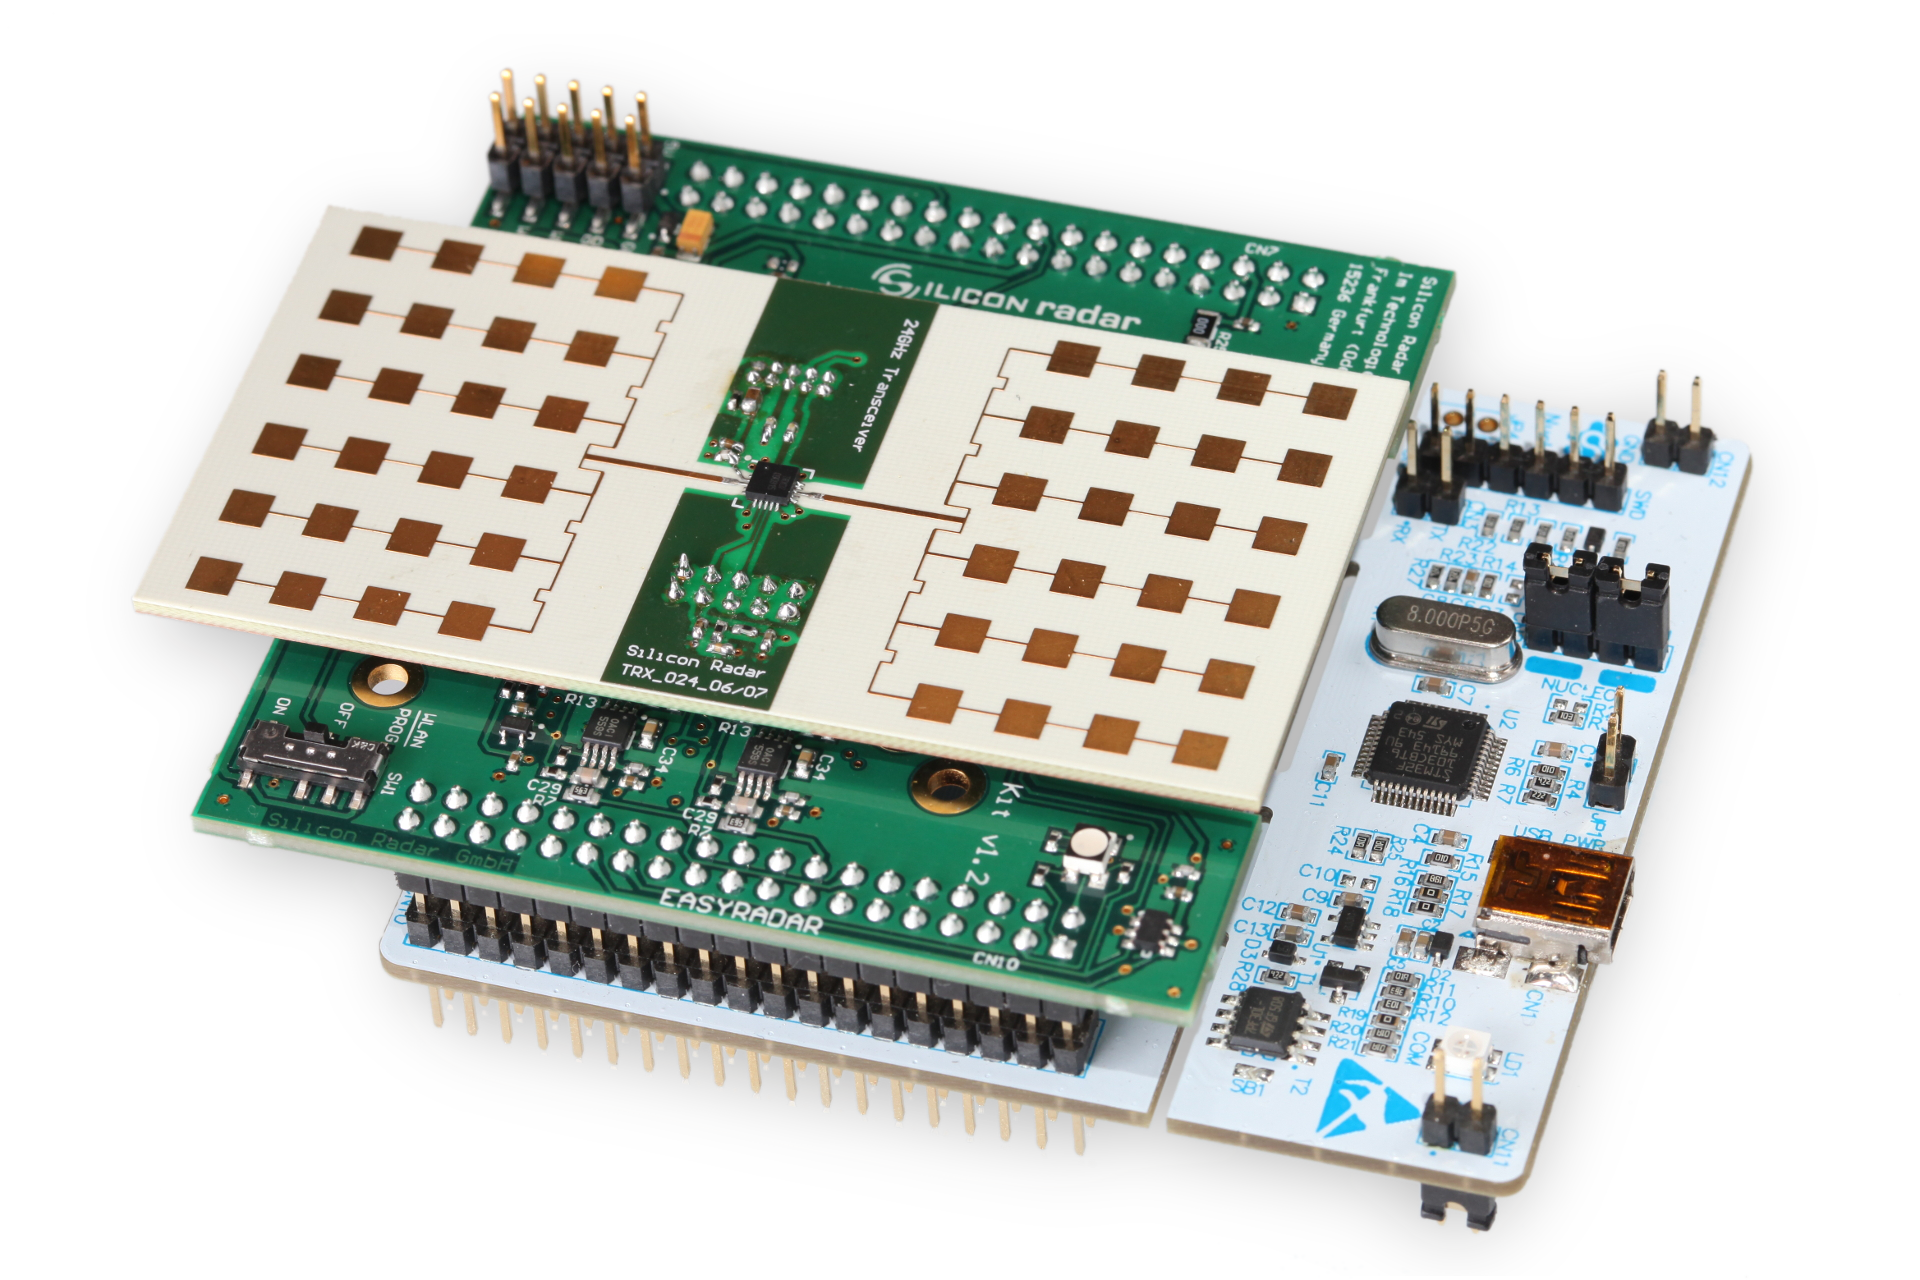
\includegraphics[width=0.6\textwidth]{../img/sidar.png}

  \caption[\sidar \cite{sidarMANOld}]{\sidar  24~GHz configuration}
  \label{fig:sidar}
\end{figure}

Direct communication with the radar board itself is not possible, or at least, the communication interface is undocumented.
Instand there is always and intermediary in the form of  STM32 Nucleo series microcontroller.
To this microcontroller does the user connect either directly with UART over USB or with WiFi over on board ESP32.
Both are relatively low bandwidth communication -- the serial maxing at baudrate of 1~000~0000.

\begin{figure}[h!]
  \centering
  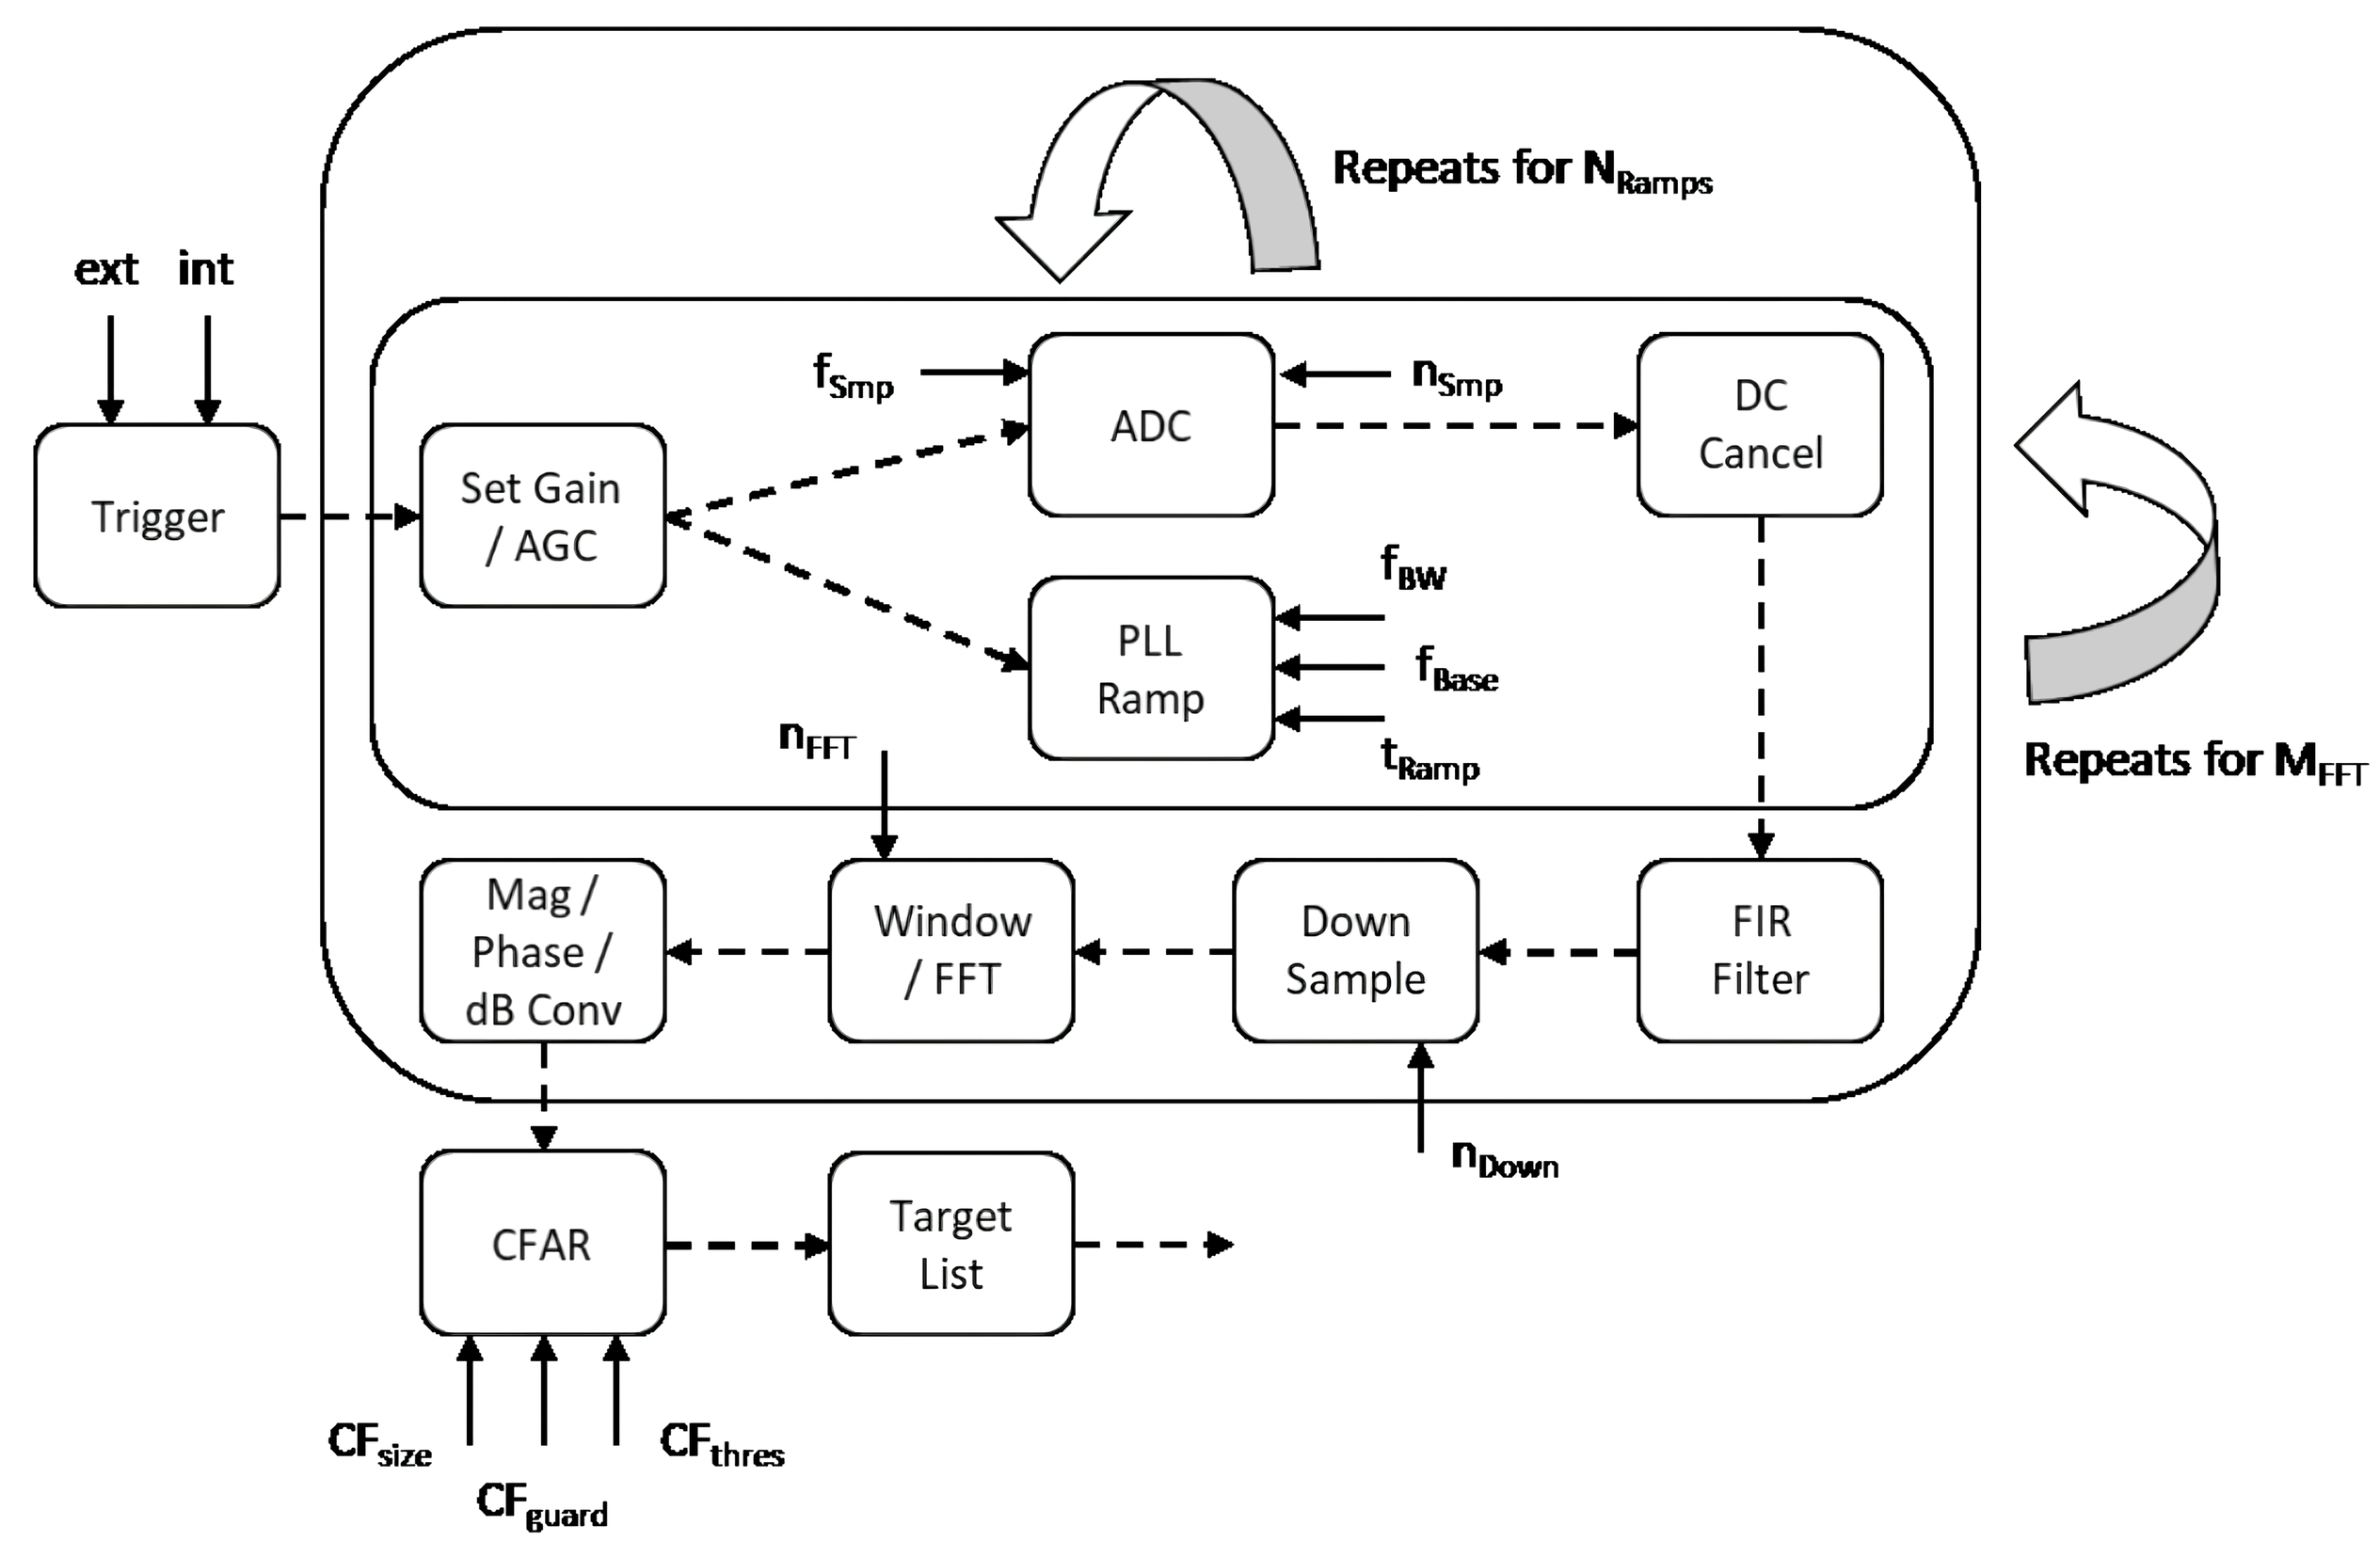
\includegraphics[width=0.7\textwidth]{../img/sidar_flow.png}
  \caption[Flow of Radar Measurement on \sidar \cite{sidarPRO}]{Flow of Radar Measurement on \sidar}
  \label{fig:sidarFlow}
\end{figure}

The devkit is designed for easy integration into existing projects; however, this unfortunately poses limitations for this thesis.
In normal operation, the radar system functions as a black box (processing schema shown in \ref{fig:sidarFlow}), implementing its own filtering, FFT, and CFAR algorithms while only reporting a target list to the user.

This entire sequence can be triggered either internally (driven by a configurable oscillator) or externally (via a GPIO pin or UART input).
Once trigger is received the device carries out a user configured number of chirps.
The chirp length is determined by the number of sampling steps and the ADC sampling time as follows:
\begin{equation}
  t_\mathrm{ramp} = \frac{t_\mathrm{ADC} \cdot  (N_\mathrm{samples} + 85)}{36\,\, \mathrm{MHz}} \,\, \mu\mathrm{s},
  \label{eq:sampling}
\end{equation}
with the manufacturer recommending an optimal time of 1~ms for good SNR \cite{sidarPRO}.

SiRad is design to leverage coherent averaging to improve SNR of the output signal where multiple ramps are broadcasted and averaged.
While this technique was found to significantly aid in measurement in a cluttered environments averages effectively destroy the information about the Doppler shift.
Additionally, due to the devkit's limited computational resources instead of continuos sawtooth waveform radars broadcasts a segmented one with significant delays in between\cite{sidarPRO}.

Unfortunately whole devkit is clearly designed primarily for range detection with little to no regard payed for speed measurement.
Not only are chirps spaced with large delays (at minimum some 19~ms) but radar doesn't even maintain constant intervals between chirps.
This is the case even when relying on manual triggering of the radar, relying on self trigger yields even worse results.

When measuring reporting interval with 20~ms trigger radar achieved average time of 20.5~ms with standard deviation of 1.3~ms.
However from time to time they were outlier when report came in only after 30~ms in worst case or 16~ms in best case measured on 5000 samples.
In order to rule out that the problem isn't only in reporting output signal from the radar was captured by Rohde \& Schwarz FSW26 Signal and Spectrum Analyzer.
By analyzing some 40 samples, measured with same triggering interval of 20~ms, the average time between chirps was 20.7~ms with standard deviation of 0.7876~ms.

Unfortunately as the radar doesn't maintain constant intervals between chirps speed measurement precision is severely limited.
This could be partially mitigated if we knew when the chirp was broadcasted, giving us ability to introduce a correction.
However no such information is provided by the radar.
Thus each chip is timestamp with it's time of arrival which is assumed to be the time of chirp broadcast.
Respectively broadcast took time a trigger period before but this shift is irrelevant to the outcome.
Using this timing information speed spectrum can still be estimated using non-uniform DFT.

Per radars manual \cite{sidarPRO} following equation was used to calculate width of a single range bin
\begin{equation}
  \Delta R = \frac{c_0 (N+85)}{2\cdot BW\cdot NFFT},
  \label{eq:rangeBin}
\end{equation}
where variable $N$ denotes number of samples and $NFFT$ number of DFT points used to calculate the spectrum.
Except the corrective constant of 85 it closely follows the formula (\ref{eq:distance3}).
As for velocity the manufacturer doesn't recommend any formula so (\ref{eq:Doppler3}) was used with $T_\mathrm{ch}$ substituted by user-chosen trigger period.
However as the minimal period of chirps is still rather high not to mention the radar doesn't maintain constant intervals between chirps, the velocity measurement is not very practical.
Were we to use 24~GHz header with 25~ms trigger we get maximal speed of 0.124~m/s and even with low 8 NFFT steps the resolution is only $0.031$~ms$^{-1}$.

\section{Outline of Chosen Configuration }


For the purpose of this project, the devkit was configured to output raw data from the 12-bit ADC in the form of in-phase and quadrature components of the signal.
This allows for a more detailed analysis of the radar system and enables the implementation of custom signal processing algorithms.
For these reasons, the default windowing and undocumented filtering was also disabled.
Device is left to be triggered by command sent over UART, which is not the most reliable method but allows for more flexibility in the configuration.

Another parameter to consider in relation to rotary application is AGC.
Using it adds two additional ramps that are used solely to set gain value but it also can lead to inconsistent weights of values between two neighboring data sets.
Former only introduces a small slowdown but the letter could be a problematic, especially since radar doesn't really report change in AGC value.
Thus its safest to turn AGC off and set the gain manually depending on how the readings appear in post processing.

It is also important to note that the radar system is not well-suited for on-the-fly configuration changes.
Applying a new configuration takes some time  and the radar does not provide any feedback to indicate when a new configuration was applied.
As a result, commonly used techniques such as alternating chirp slope or frequency modulation are not feasible.

In regards to the output format, the radar system supports two options: binary and TSV.
Since the output speed does not differ significantly between the two, the primary deciding factor is the ease and speed of parsing.
Even though MATLAB is not particularly optimized for parsing binary data, it still processes binary output approximately 40\% faster than human-readable TSV data.

Other parameters such as sampling frequency, number of samples and so on are left to the user to configure.
Setting these strongly depends on what header is used and what environment is the radar used in.
Thus making their configuration static wouldn't be a good idea.


\section{24~GHz Header}

Center of 24~GHz header is a SISO TRX-024-007 transceiver which integrates low noise amplifier, frequency mixer, filters and VCO into a single chip.
It is primarily designed to operate in the ISM band (24.0--24.25GHz), with an additional ultra-wideband mode supporting 23--26~GHz \cite{sidarTRX24}.
On the \sidar there is no distinction made between  those two modes and the user is free to set any bandwidth \cite{sidarPRO} .
The transmitter output power ranges from 2.5~dBm to 6~dBm, depending on the configuration \cite{sidarTRX24}.
A maximum range of 400~m is advertised \cite{sidarMANOld}, though this is likely under ideal conditions when observing a large target.
Also as previously stated the radar will operate on much lower sampling frequency than needed to achieve such results.


As shown in Figure \ref{fig:sidar}, the chip is connected to two microstrip patch antennas.
The patches are arranged in a relatively standard configuration, forming a 6×4 array with spacing approximately equal to half the wavelength at 24~GHz.

Since the manufacturer did not provide any information about the radiation pattern of the array, a simulation was conducted using the CST simulation suite.
Additionally, the manufacturer did not disclose the substrate parameters for the radar board specifically.
Fortunately, the TRX-024-007 datasheet includes a board stack-up for the chip's evaluation board.
It was assumed that the same stack-up would be used—18~$\mu$m copper for the traces and ground plane, with a 250~$\mu$m thick Rogers RO4350B substrate \cite{sidarTRX24}.

\begin{figure}[ht!]
  \centering
  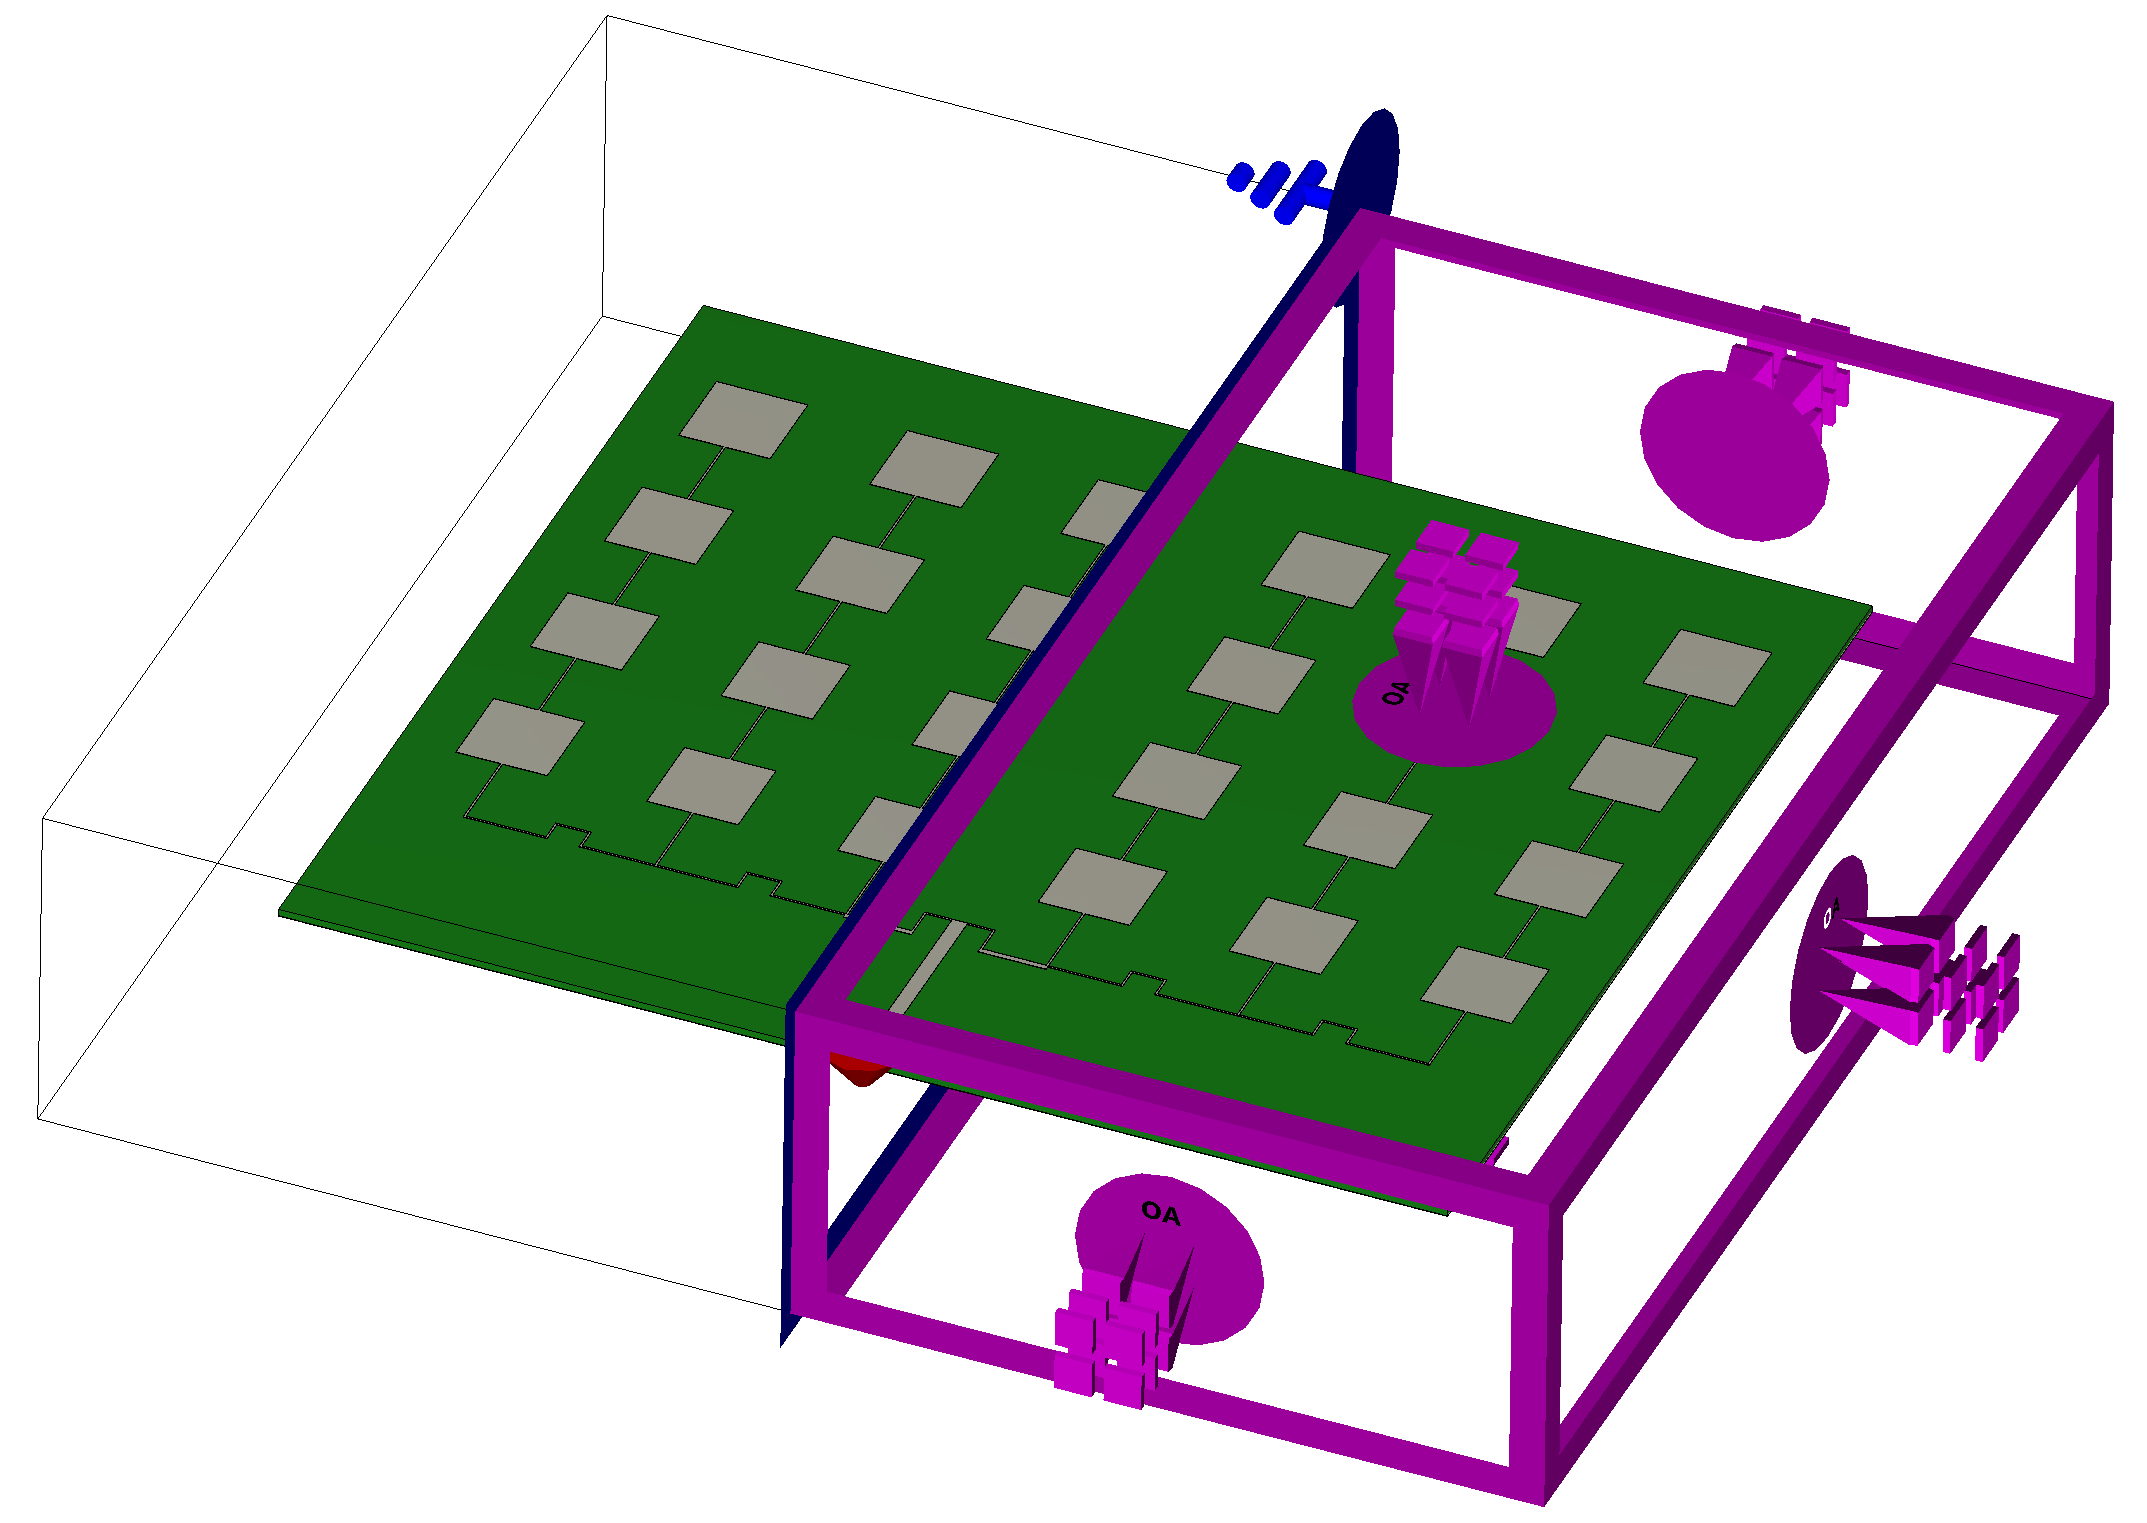
\includegraphics[width=0.6\textwidth]{../img/boundaries.png}
  \caption[Simulated 24 GHz header with boundary conditions showed]{Simulated 24 GHz header with boundary conditions showed}
  \label{fig:boundaries}
\end{figure}

After measuring the dimensions of the array using an optical microscope, the entire array was redrawn in CST Studio.
Figure \ref{fig:boundaries} shows the applied boundary conditions: the antenna was placed in open space, and an $H=0$ condition was set along the symmetry plane to speed up the simulation.

After performing a standard time-domain simulation with an excitation signal ranging from 0 to 26GHz, the antenna array exhibited a minimum reflection coefficient $s_{11} \doteq -26.4 \mathrm{~dB}$ at 23A.478~GHz with second minimum at 24.518~GHz (Figure \ref{fig:s11}).
Lack of minimum at 24~GHz may be attributed to measurement difficulties (The etching quality of the copper traces was suboptimal.) and the neglecting variations of substrate parameter due to interactions of different layers.

At both frequencies with minimal reflection, a far-field radiation pattern was calculated.
For clarity, only the 24.518~GHz pattern is shown in Figure \ref{fig:farfield3d}.
The main lobe width was measured at approximately 16 degrees (Figure \ref{fig:farfield180}) along the 180-degree norm (for orientation refer to the red cone on the PCB), with a peak gain of 18.6~dBi and side-lobe suppression of -13~dB.
For the 90-degree norm, the main lobe width (Figure \ref{fig:farfield90}) was 30 degrees, with side-lobe suppression of -10~dB.

\begin{figure}[h!]
  \centering
  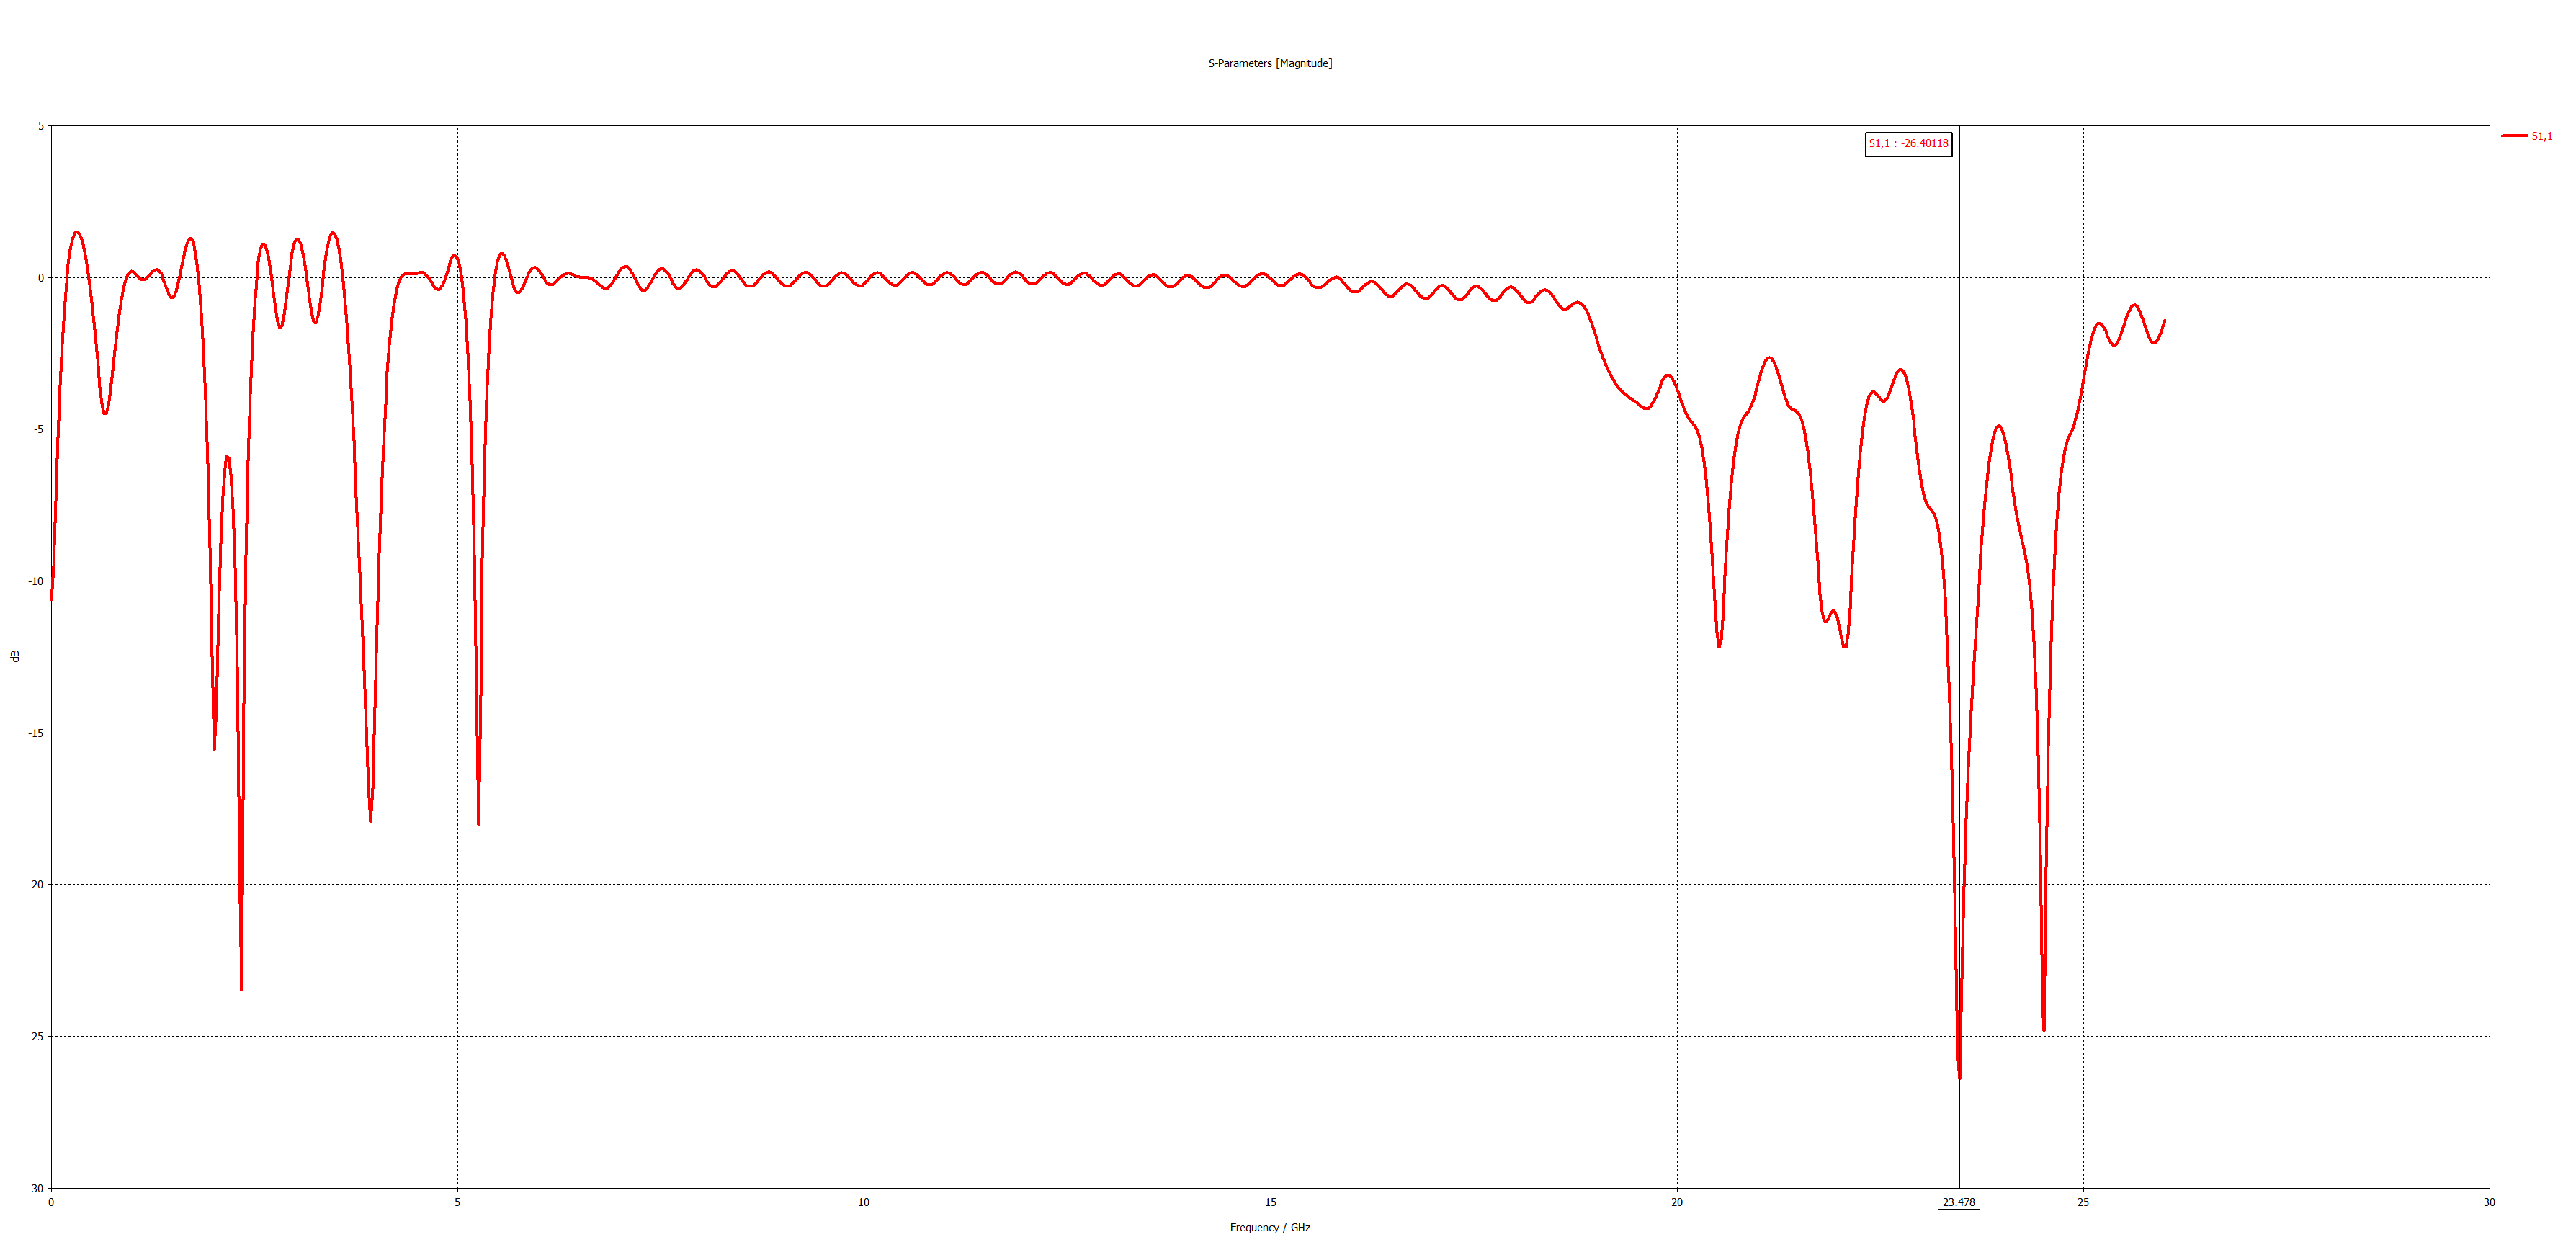
\includegraphics[width=0.9\textwidth]{../img/s11.png}
  \caption[$s_{11}$ parameter of the 24~GHz header]{$s_{11}$ parameter of the 24~GHz header}
  \label{fig:s11}
\end{figure}


\begin{figure}[h!]
  \centering
  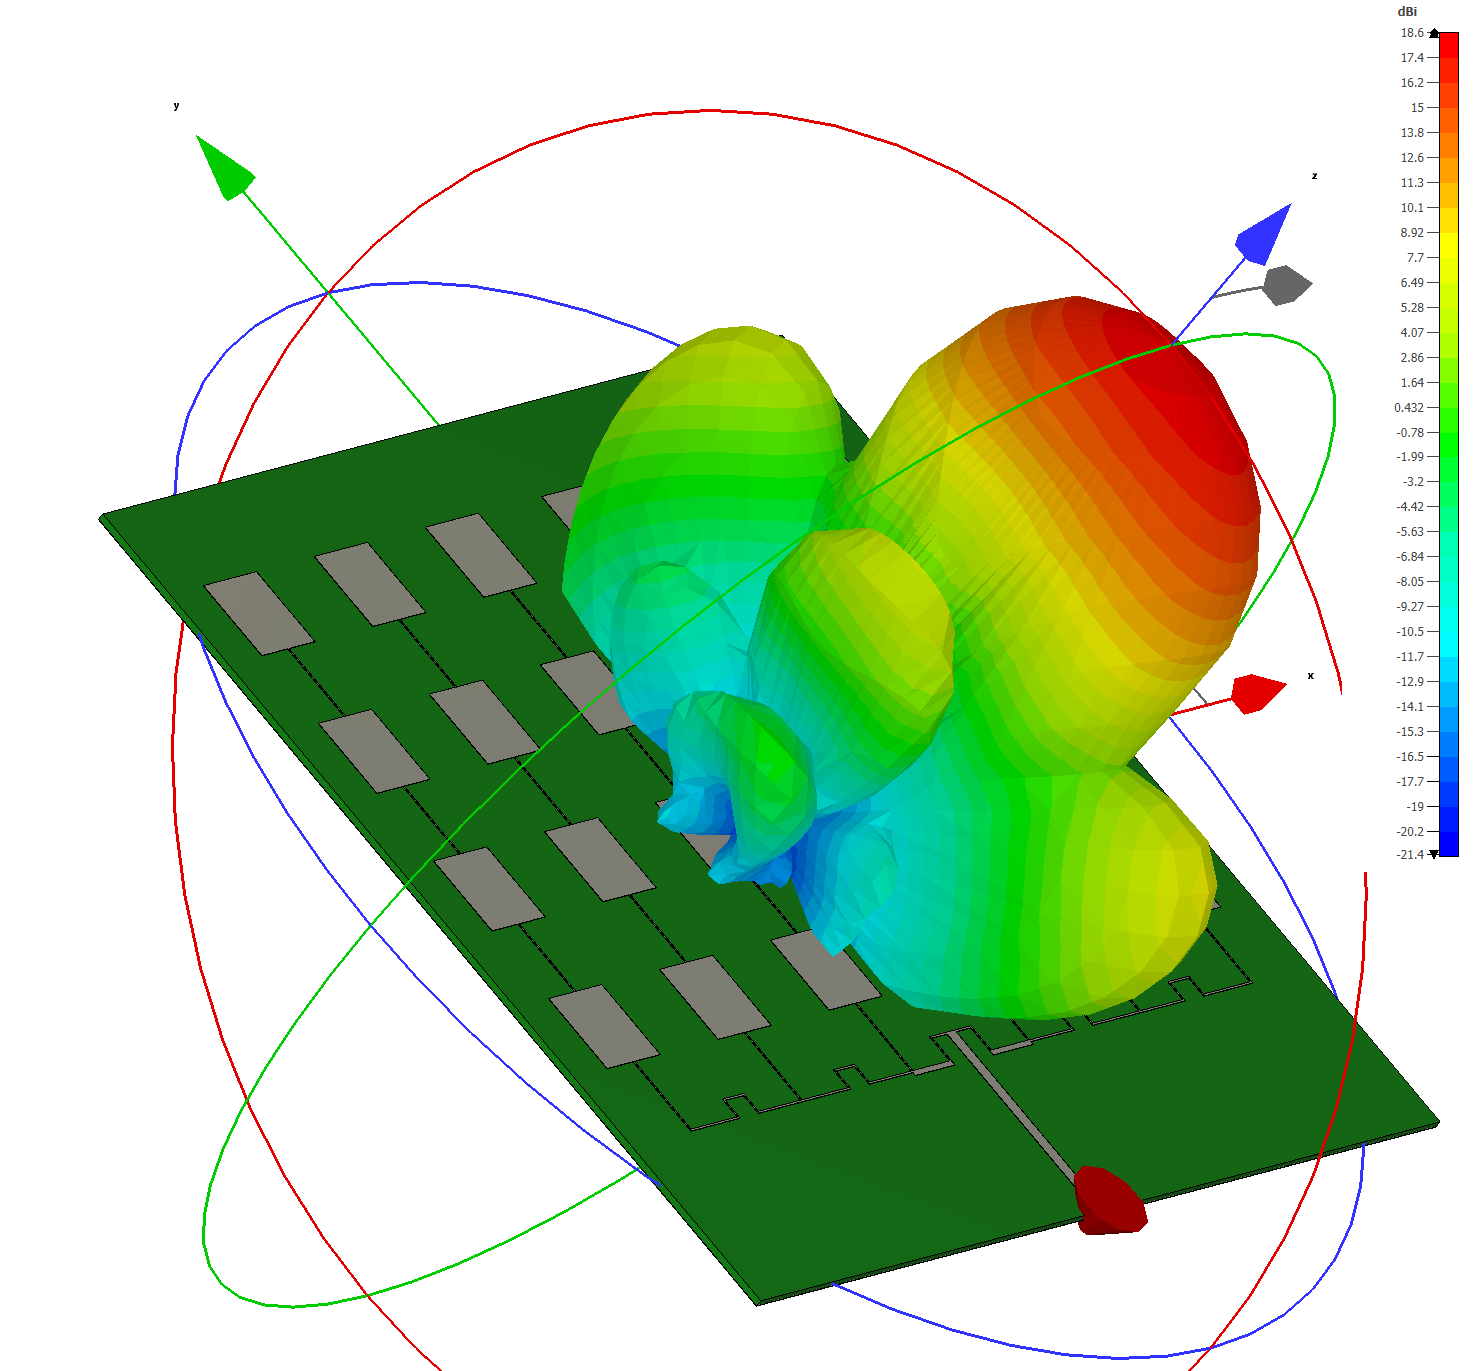
\includegraphics[width=0.43\textwidth]{../img/farfield3d.png}
  \caption[Radiation pattern of 24~GHz header -- 3D view]{Radiation pattern of 24~GHz header -- 3D view}
  \label{fig:farfield3d}
\end{figure}

\begin{figure}[h!]
  \centering
  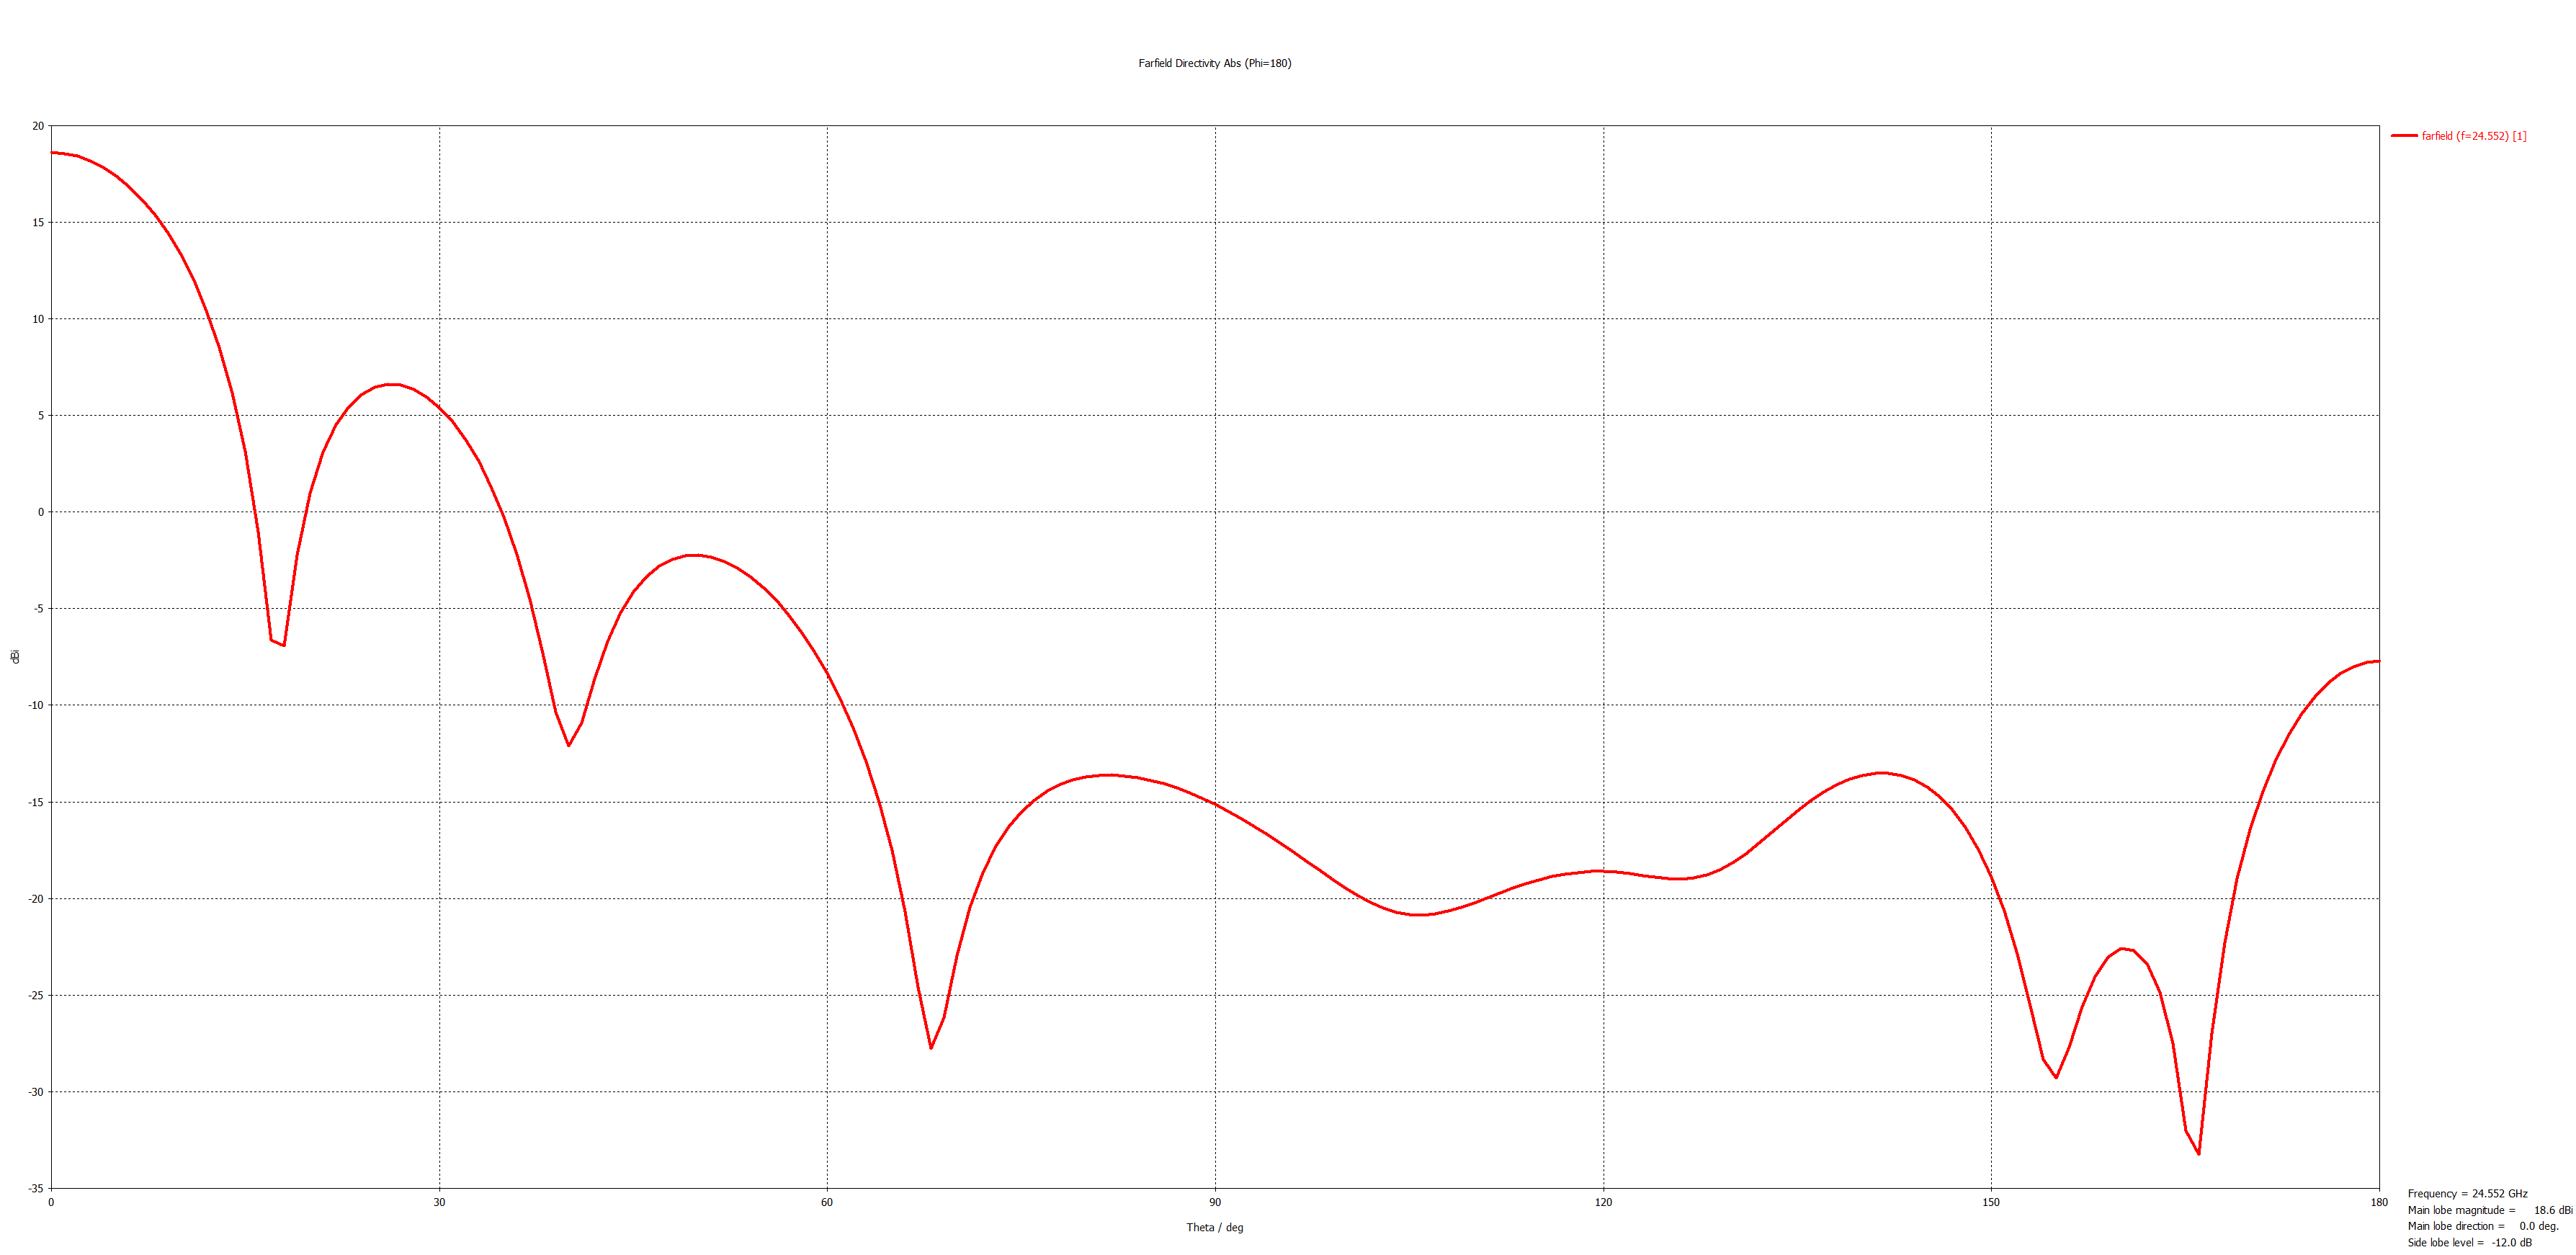
\includegraphics[width=0.9\textwidth]{../img/farfield180.png}
  \caption[Radiation pattern of 24~GHz header -- 180° norm]{Radiation pattern of 24~GHz header -- 180° norm}
  \label{fig:farfield180}
\end{figure}

\begin{figure}[h!]
  \centering
  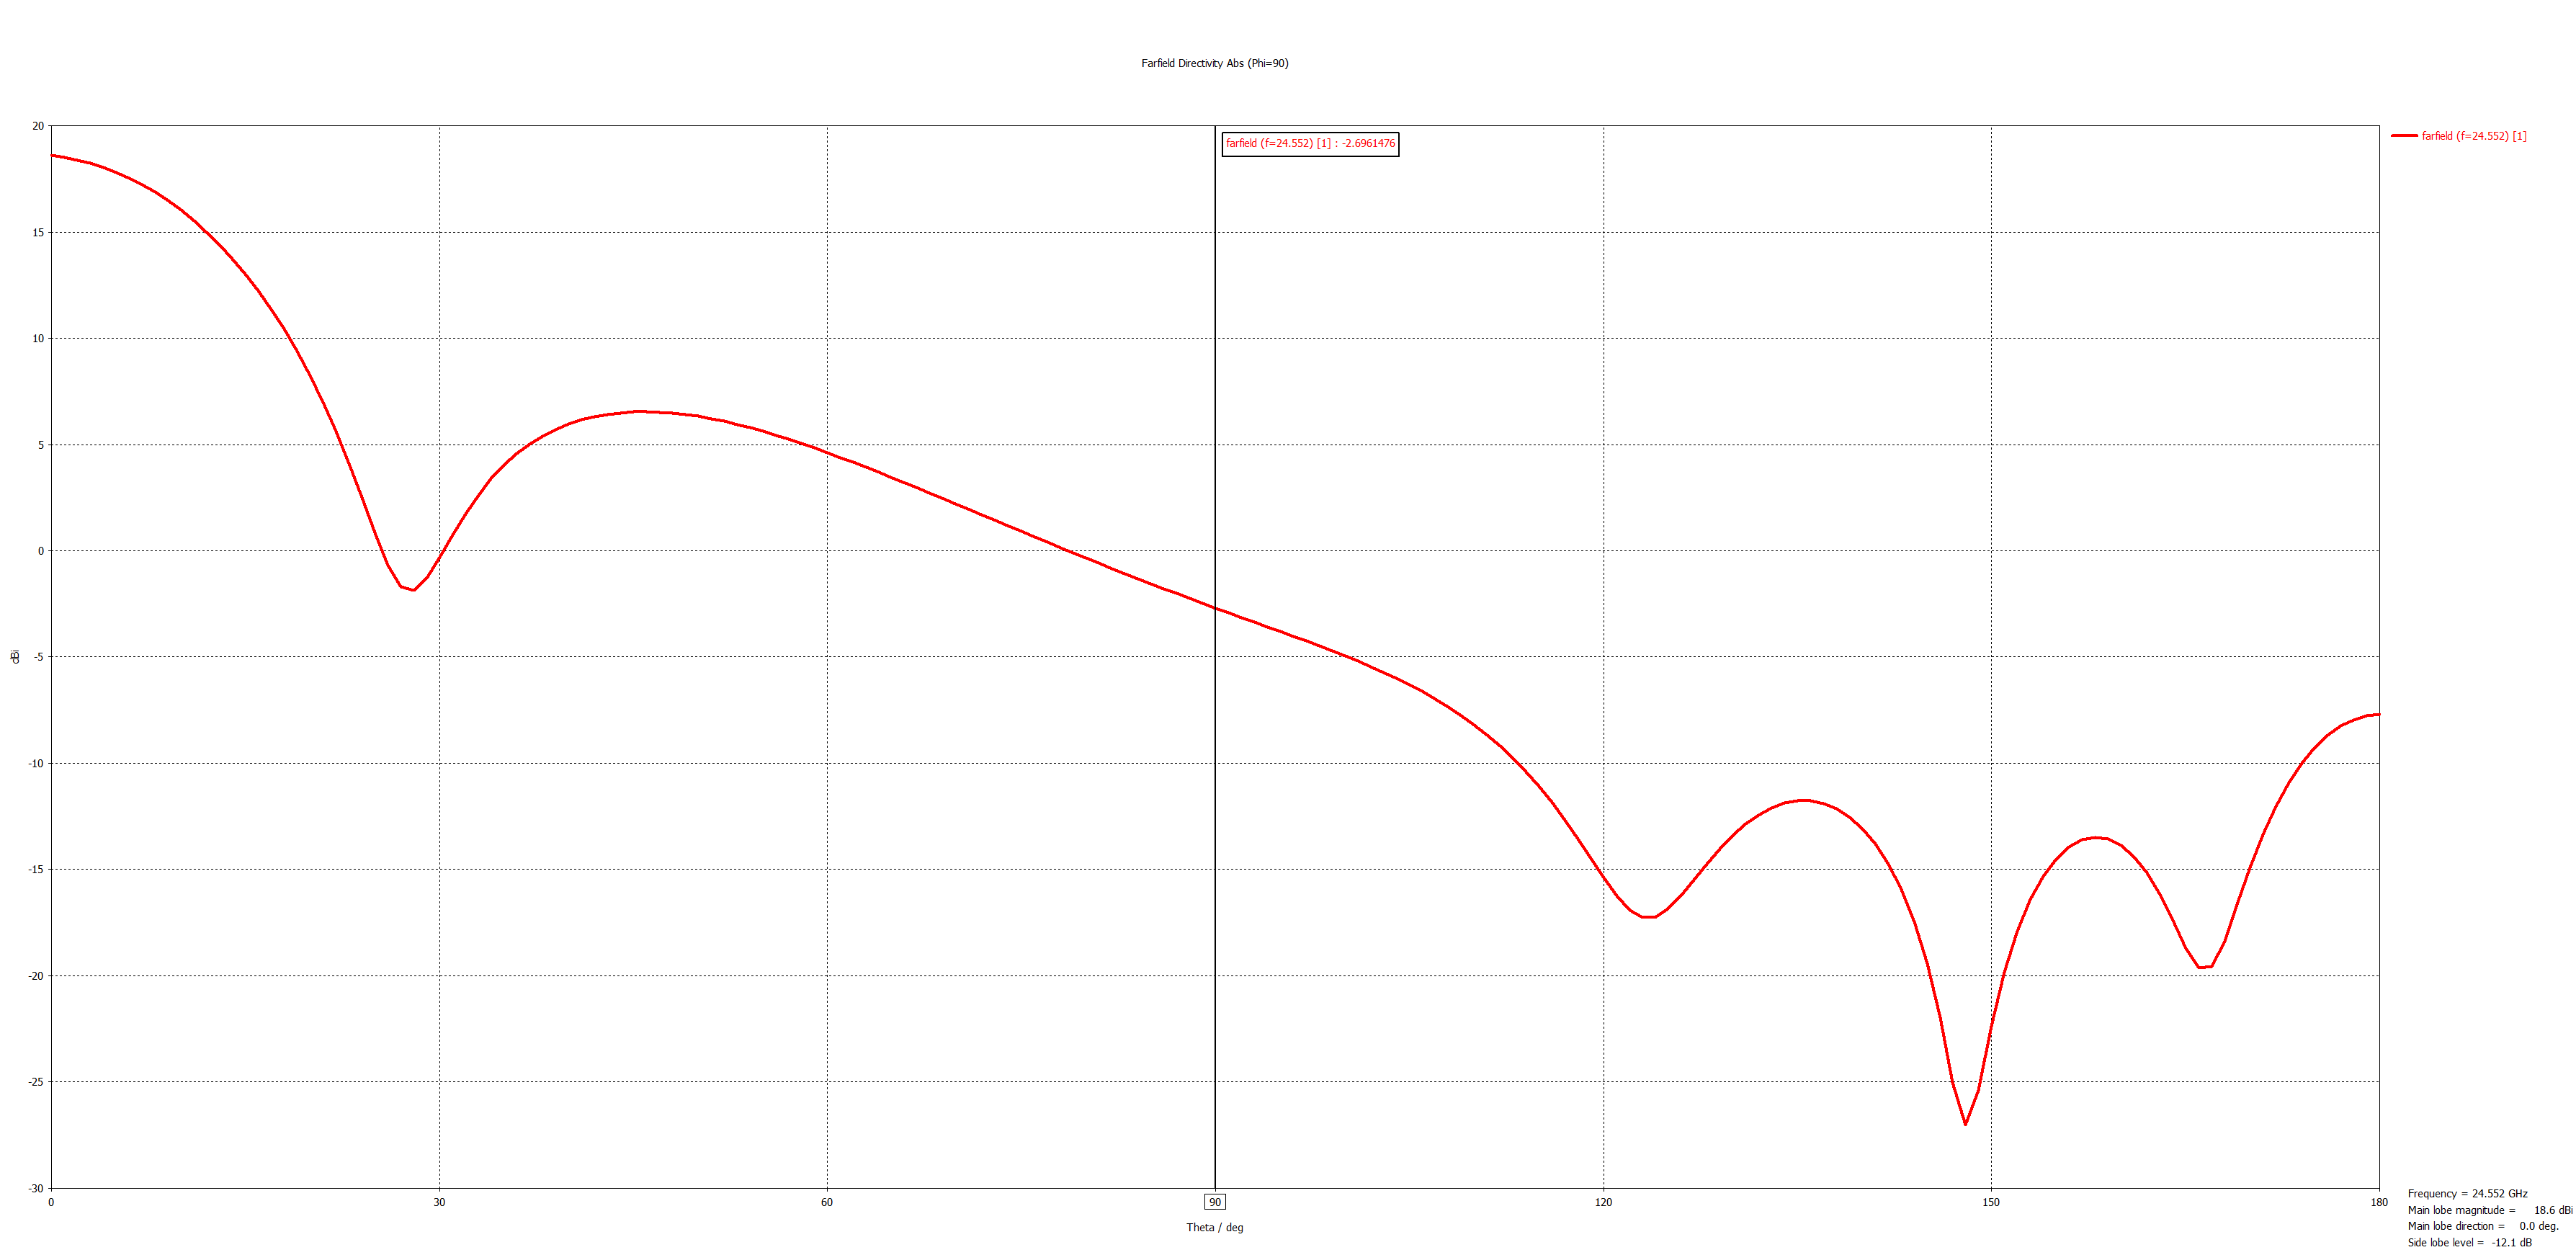
\includegraphics[width=0.9\textwidth]{../img/farfield90.png}
  \caption[Radiation pattern of 24~GHz header -- 90° norm]{Radiation pattern of 24~GHz header -- 90° norm}
  \label{fig:farfield90}
\end{figure}


\section{122~GHz Header}

\begin{figure}[h!]
  \centering
  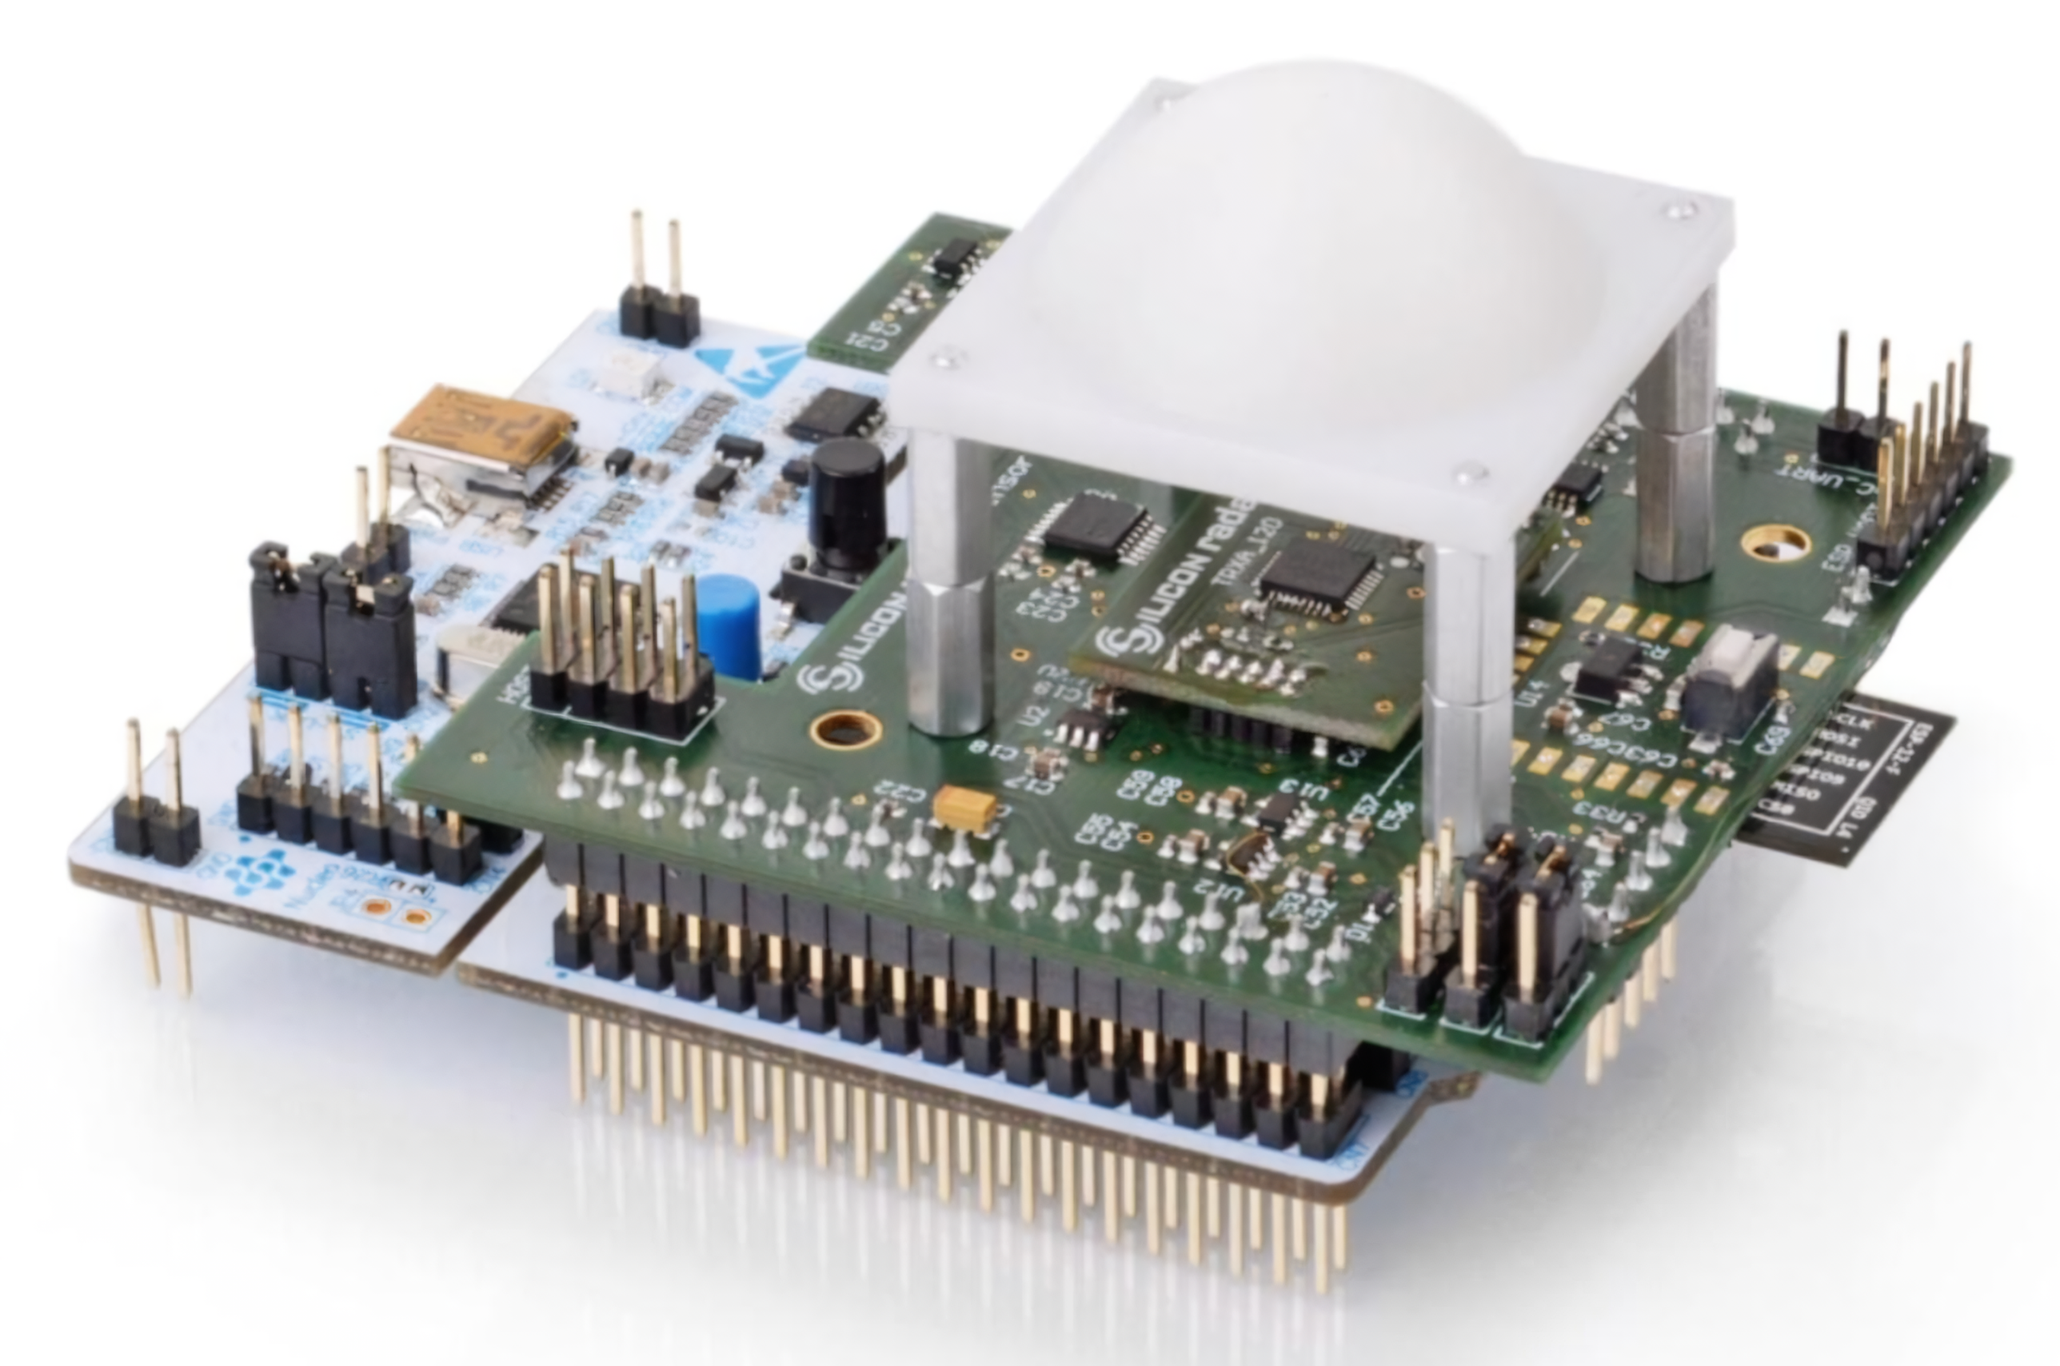
\includegraphics[width=0.5\textwidth]{../img/sidar122.png}
  \caption[\sidar with 122~GHz header \cite{sidarPRO}]{\sidar with 122~GHz header}
  \label{fig:sidar122}
\end{figure}

The 122~GHz header is based on the TRX-120-001 transceiver, which, in addition to the essential components required for RF transmission and reception, also incorporates two on-chip antennas.
It's designed to operate in the 122-123~GHz band, with output power ranging from -7~dBm to 1~dBm \cite{sidarTRX122}.
The chip is capable of detecting large targets at distances of up to 40~m \cite{sidarMANOld}.

Out of the box performance of the system is quite bad (Figure \ref{fig:sidar122rad}) with width of the main lobe being roughly $\pm40\text{°}$ in both E-plane and H-plane \cite{sidarTRX122}.
However, this can be significantly improved using the supplied collimator lens, reducing the main lobe width to $\pm4\text{°}$ \cite{sidarTRX122col} (see Figure \ref{fig:sidar122rad}).


\begin{figure}[h!]
  \centering
  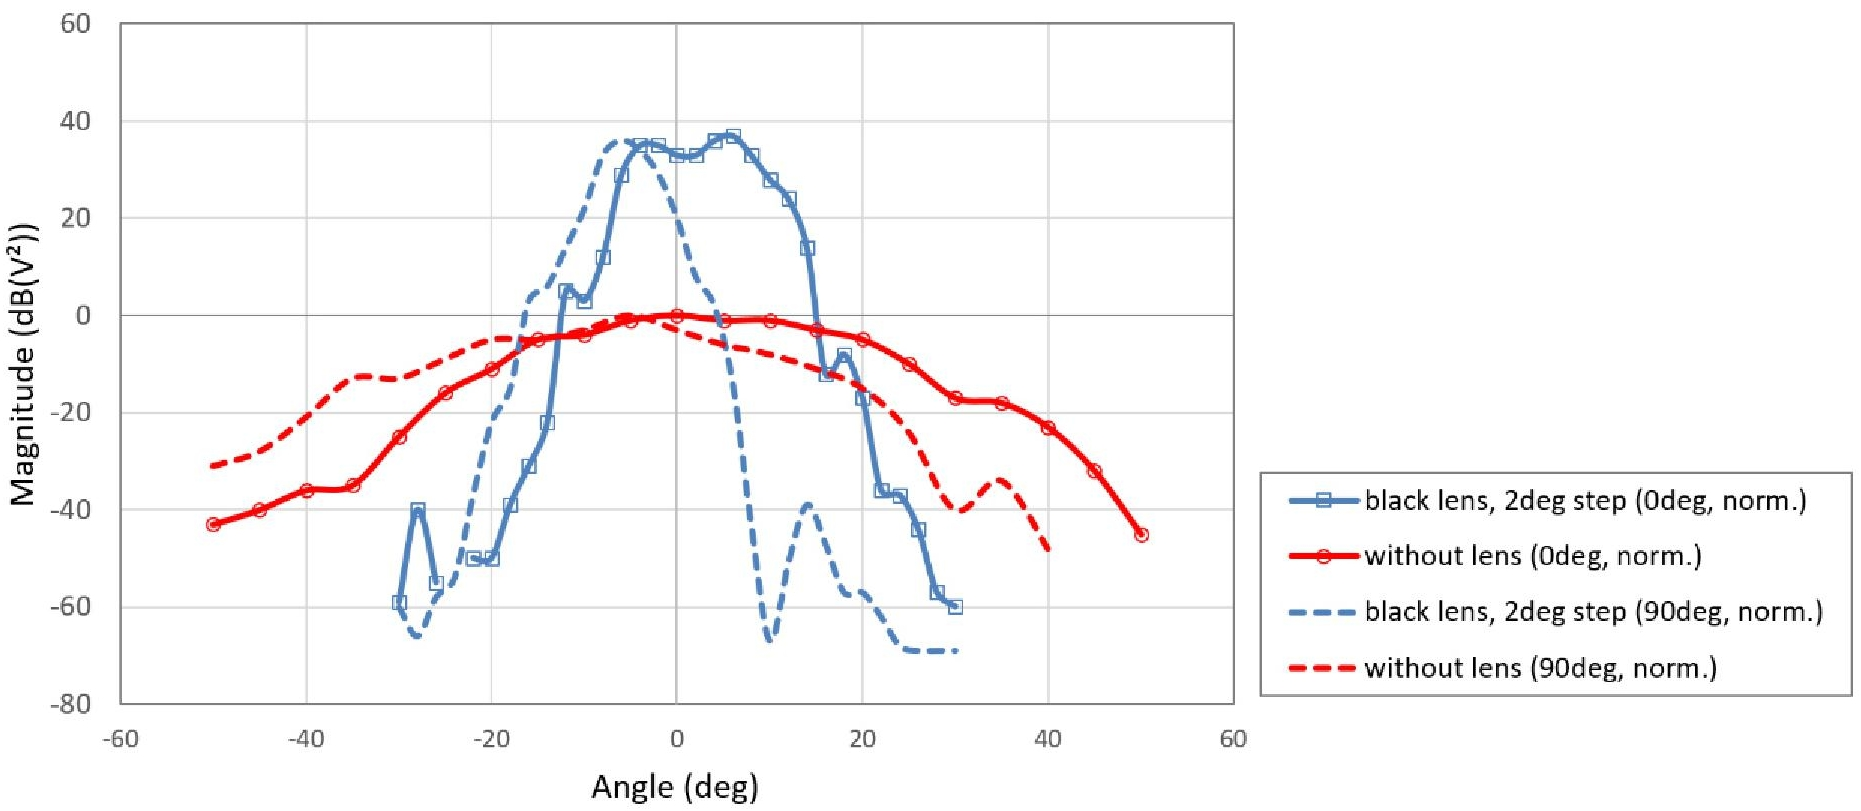
\includegraphics[width=0.85\textwidth]{../img/sidar122rad.jpg}
  \caption[Radiation pattern of 122~GHz header comparison \cite{sidarTRX122col}]{Radiation pattern of 122~GHz header comparison}
  \label{fig:sidar122rad}
\end{figure}



\chapter{Rotary Platform}

Following chapter outlines design process and the operation of a rotary platform specifically designed for \sidar radar system.


\section{Platform Construction}

As the platform needs to transmit data from the rotating section to the stationary base, a slip ring is required.
Due to the relatively low transmission speed of the radar and the absence of special requirements such as waterproofing, an affordable model, UH3899-01-0810 from Senring, was selected.
It is a classical contact slip ring that features a dedicated USB~2.0 connection along with 8 additional signal wires, with an advertised insertion loss of less than 2~dB \cite{slipring}.
More problematic than loss is however cross talk between signal wires when stepper motor responsible for pitch control of the radar is running.
This necessitated an addition of small capacitor to the endstop signal pin to filter out high frequency noise.

While USB~2.0 connection doesn't seem affected by the crosstalk it's connection still isn't ideal.
Without signal conditioner connected directly to the slipring output signal quality is bad enough that direct connection to PC is needed.
And even then depending on PC's wiring some ports might exhibit issues.
In addition the manufacturer opted for a non-standard male-male USB~2.0 connection, requiring a female-female adapter to connect the radar to the slip ring.

Due to the relatively low angular resolution of the radar, high platform precision was not a requirement.
A basic 200-step stepper motor with a step size of 1.8\text{°} was deemed sufficient.
In case user would require more granular control over the position it can be facilitated by microstepping.

Similarly high-speed movement is unnecessary for this application.
As was already outlined the radar is capable at best of 50~Hz update rate.
With such update frequency even at low 8~RPM we travel a degree under 21~ms too right on the edge of what is radar capable.
Also at these RPMs standard 40~mm NEMA17 stepper motors are powerful enough to turn the splipring.

The rest of the design is relatively simple.
The fixed section mounts the slip ring with the stepper motor positioned underneath, directly driving a shaft connected to a rotating base.
The connection is secured using long M4 set screws that pass through the base the slip ring and hold the shaft in place.
A 3D-printed housing serves only as a centering guide and is not responsible for connecting shaft to the rotary base.

The rotating section features a simple A-frame design that elevates the radar, which is mounted on bearings, allowing it to tilt freely.
To control the pitch, a second stepper motor is mounted on the rotating platform and linked to the radar via a 2:1 down-gearing ratio using a standard 8~mm belt.
An optical endstop, used for homing of the platform, is mounted on the second support strut.

Unfortunately while the platform offers some ability to tension the belt in currently printed configuration the range is not sufficient to fully tighten the belt.
While slippage is not a problem radar there is some slack in radar's tilt.
However as the radar's capabilities in pitch direction aren't particularly high it was decided not to reprint the whole assembly, only to fix issue in supplied 3D models.

Given that  mechanical stresses are minimal, most parts can be 3D-printed using standard PLA filament.
The only non-3D-printed components are the screws, bearings, and stepper motors.
The final assembly (Figure~\ref{fig:side_by_side}) measures approximately 33~cm in height and has a footprint of $20\times20$~cm.

\begin{figure}[h!]
  \centering
  \begin{subfigure}[b]{0.45\textwidth}
    \centering
    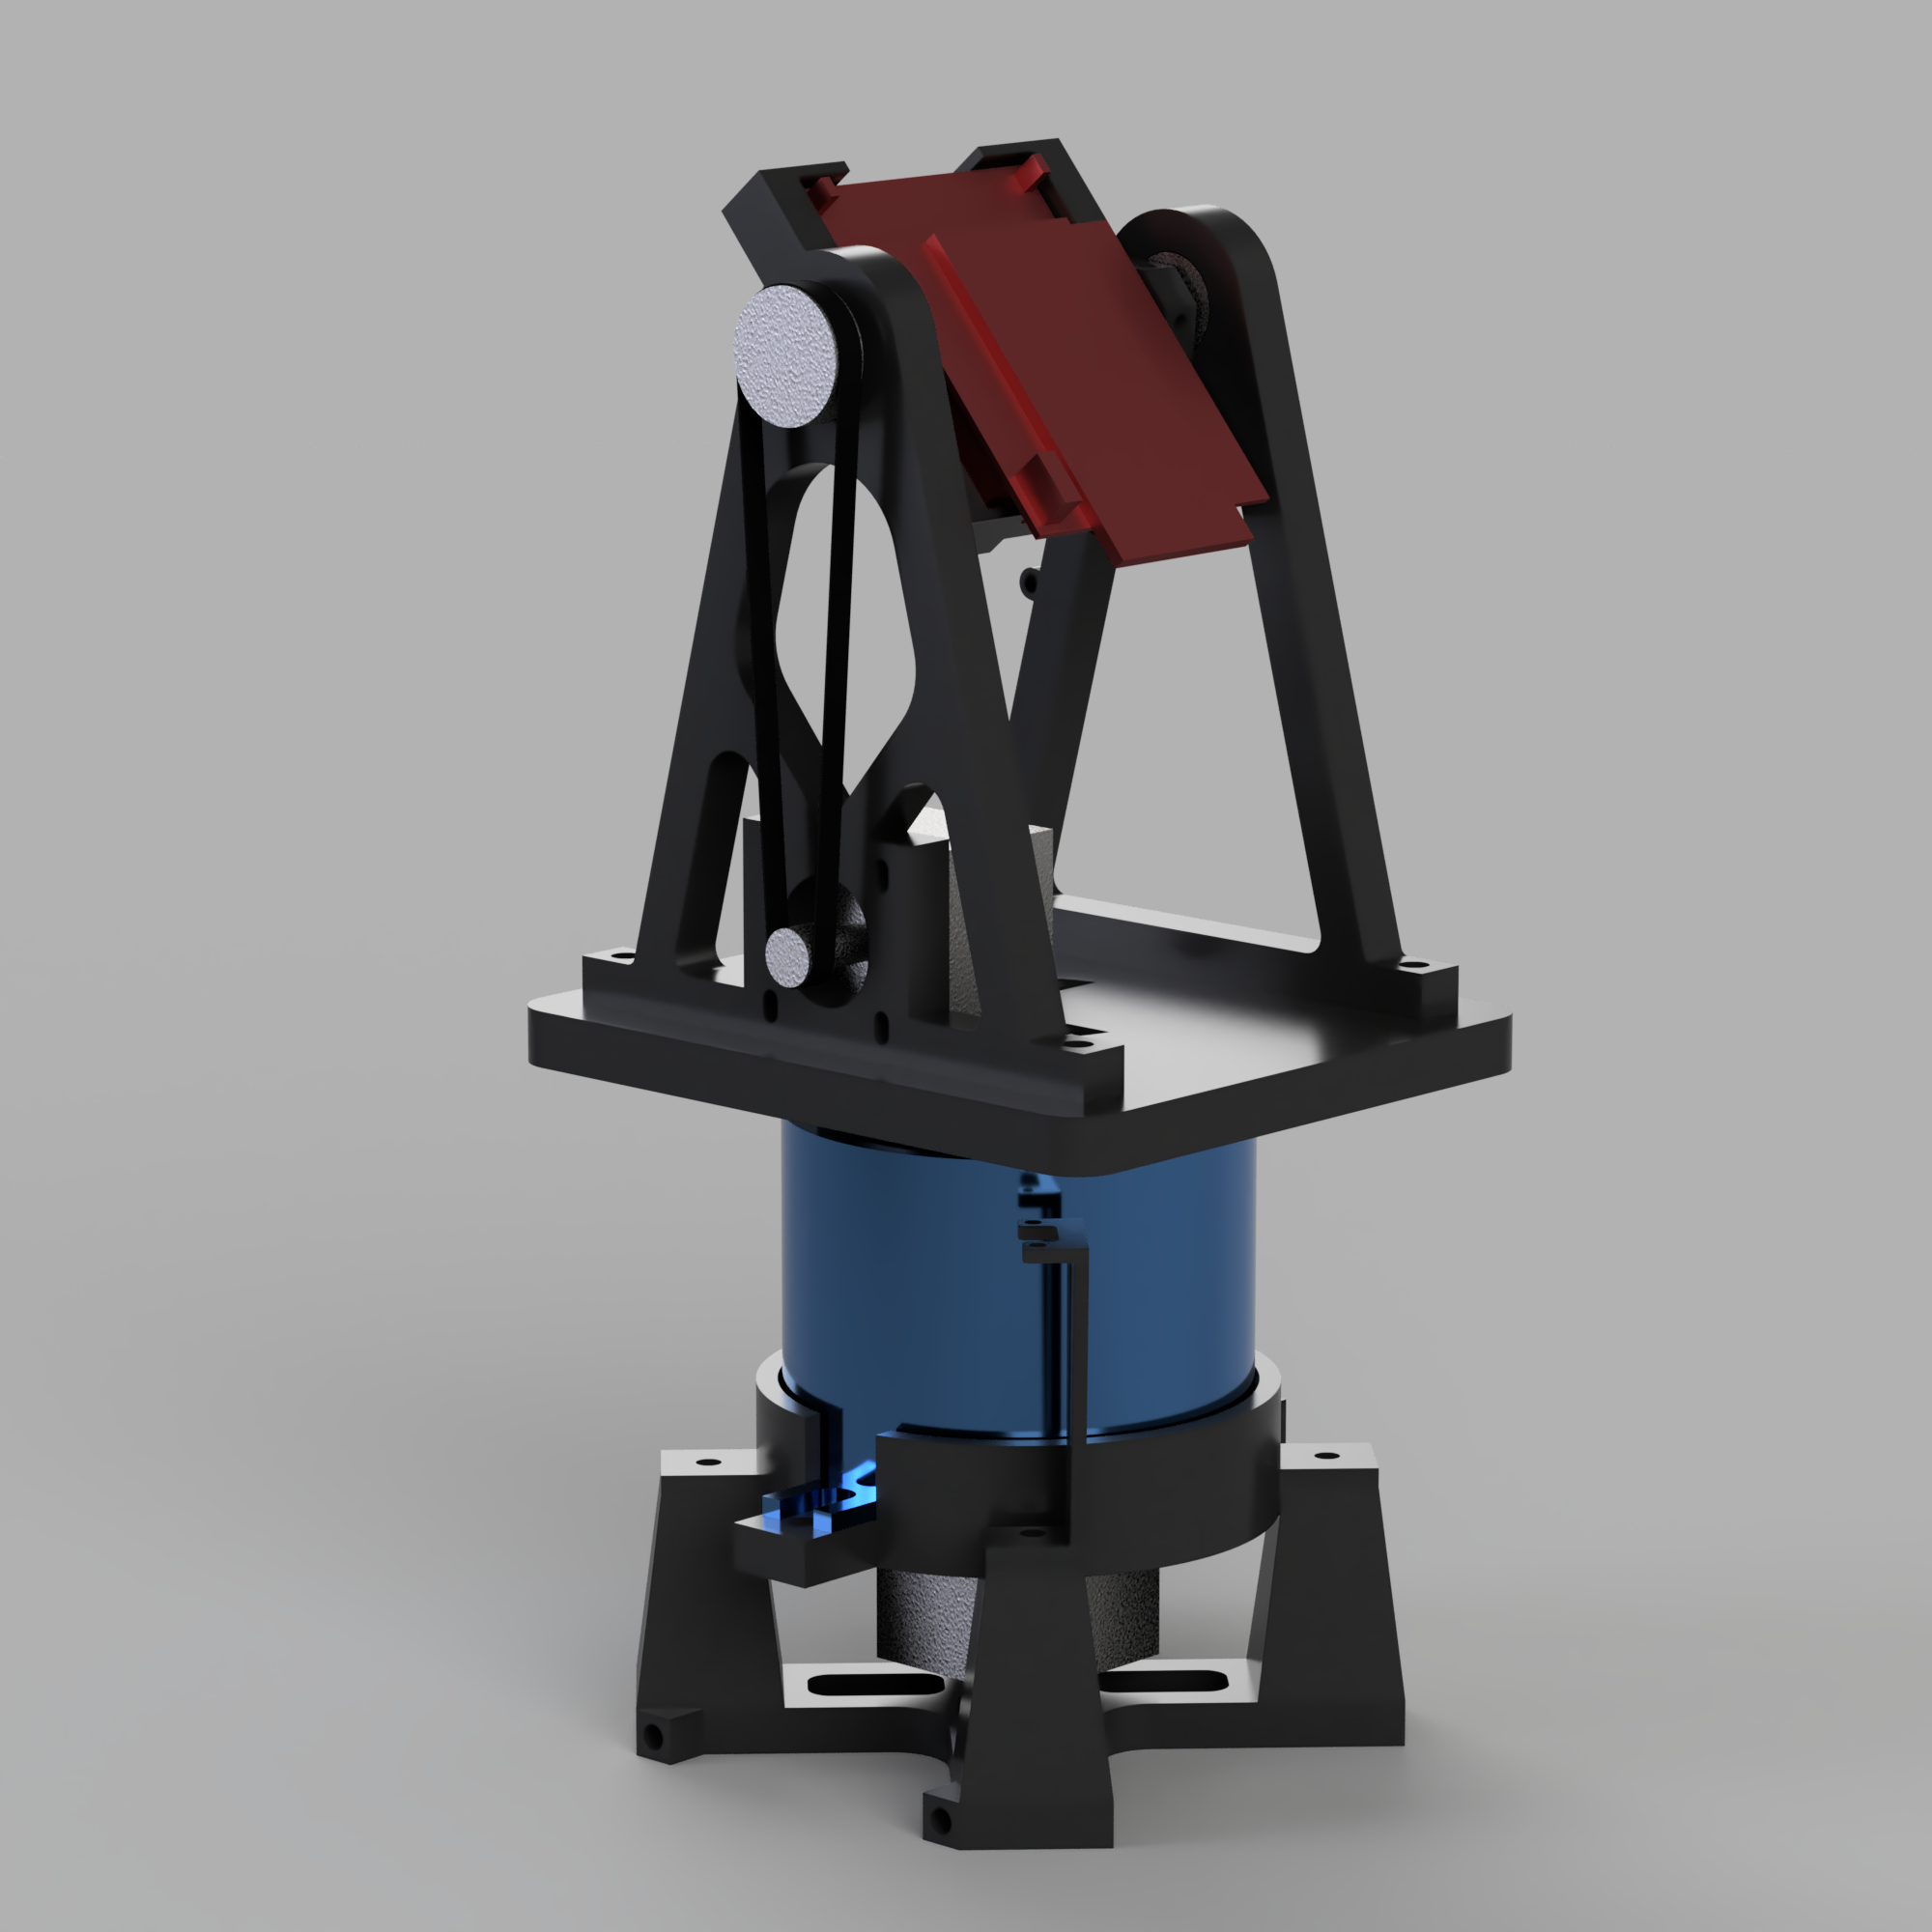
\includegraphics[width=\textwidth]{../img/whole_assembly_2.png}
    \caption{3D render}
  \end{subfigure}
  \hspace{0.05\textwidth} % Adjust spacing
  \begin{subfigure}[b]{0.45\textwidth}
    \centering
    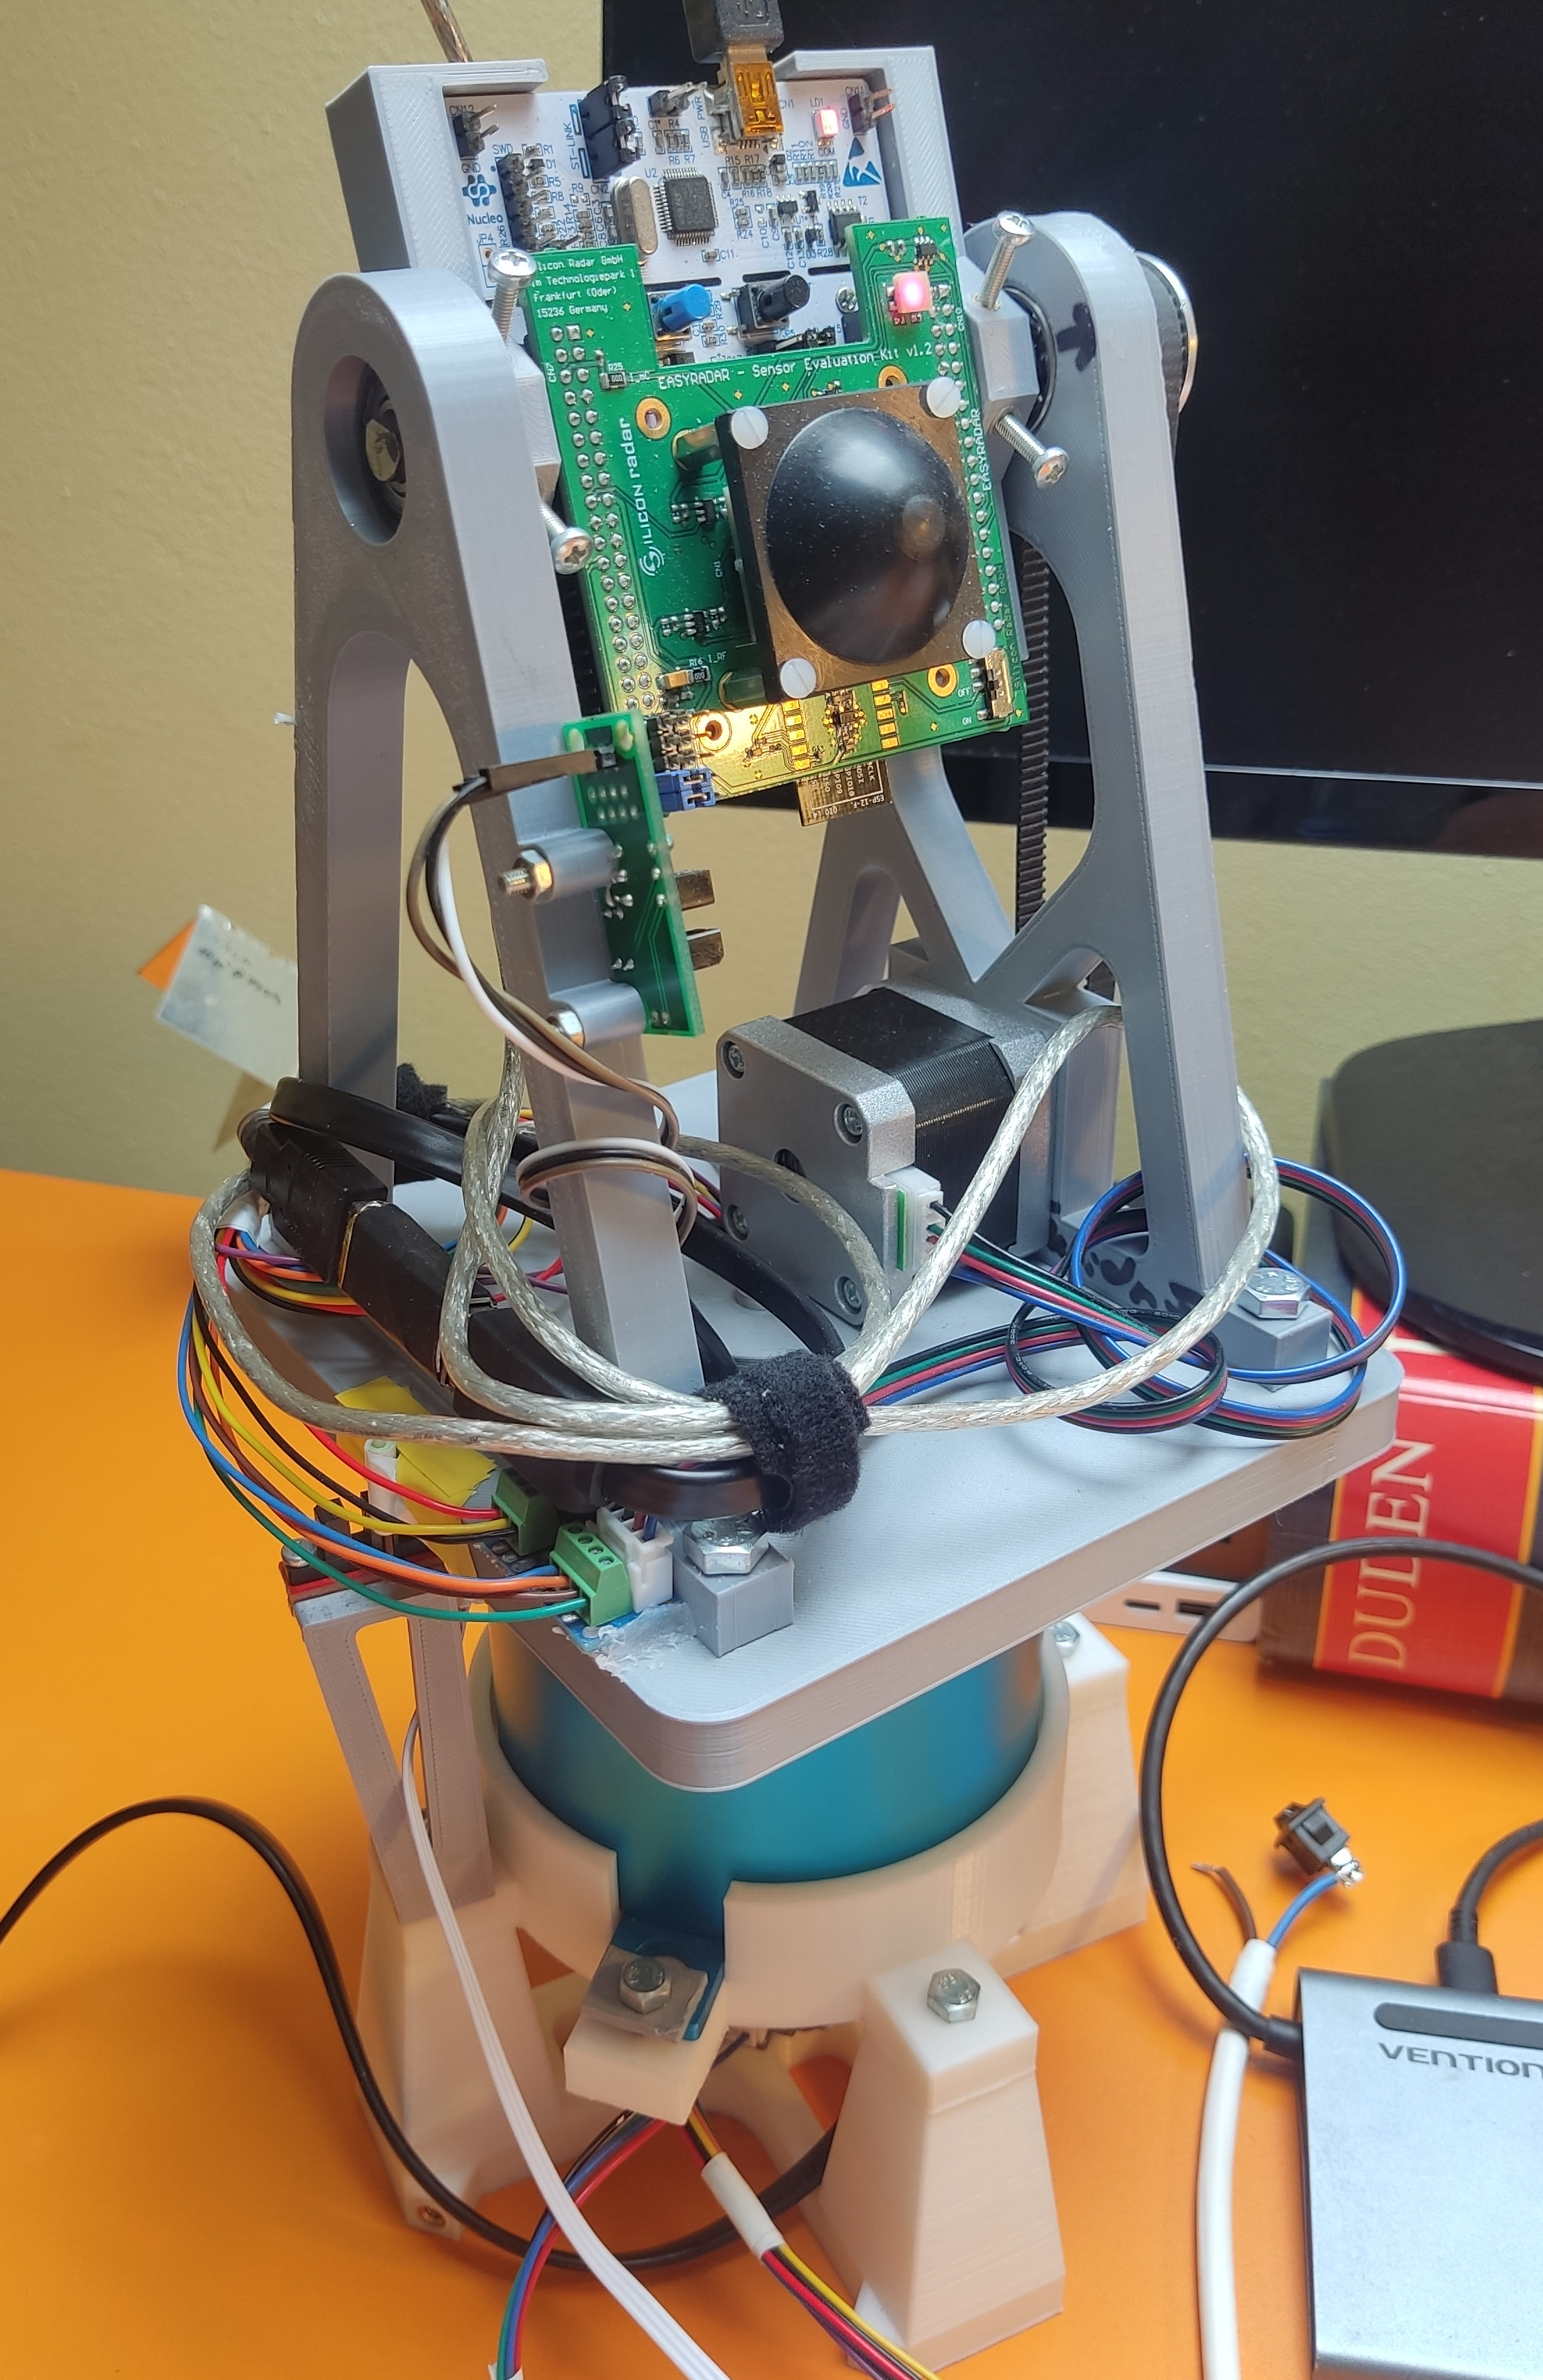
\includegraphics[width=0.75\textwidth]{../img/assembly_photo.jpg}
    \caption{Photo}
  \end{subfigure}
  \caption{Form of the final assembly}
  \label{fig:side_by_side}
\end{figure}


\subsection{Platform Electronics}

The electronic aspect of the platform is relatively simple.
Only two main problems needed to be tackled -- driving the stepper motors and implementing a homing mechanism.

Given the low load on the stepper motors and the platform's inability to accumulate significant momentum, a basic stepper driver without feedback control was deemed sufficient.
For this purpose the A4988 stepper driver was chosen due to its low cost, microstepping capabilities and basic current control \cite{a4988}.
A minor drawback is the lack of feedback from the driver to the microcontroller, including the absence of stall detection.
To simplify the design, A4988 development kits were used and soldered onto a prototyping board, eliminating the need for a custom PCB.
In addition if the need arieses A4988 development kit can be replaced by one with a different IC, such as TCM2209, as manufacturers keep the same pinout and dimensions on these complementary kits.
This might be necessary in application where platform loudness would be a serious problem as A4988 produces rather noisy driving signal leading to even 20 dB higher operating volume \cite{a4988_sound}.

For homing implementation, two potential solutions were considered: Hall effect sensors and optical gates.
Hall effect sensors offer the advantage of angle sensing, allowing correction for positional drift during operation; however, they require precise alignment.
If the orthogonal Hall effect sensor is not perfectly placed along the axis of rotation, calibration becomes necessary \cite{hall}.
While feedback would be beneficial, the microcontroller already tracks each step taken by the motor during normal operation, making it possible to determine the platform's position purely in software.
Thus for simplicity and ease of integration, optical gates were selected.

The system is controlled by an ESP32 microcontroller.
The ESP32-C6 version was chosen due to the author's extensive experience with this particular model.
Still since the system does not require specialized peripherals or high processing power most other microcontrollers could have been use instead.

\section{Platform Software}

Given its widespread adoption as an industry standard for controlling multi-axis machines, G-code over serial is a natural choice for the platform's communication format.
Beyond the basic functionality typically offered by G-code interpreters, the platform must support additional features to reduce the user's manual control burden.
These features include common features like defining movement limits, absolute/relative positioning mode, spindle mode or enabling automatic homing.
Lastly the platform should support a programming interface that will allow application to send whole choreography of movements to the platform at ones and from that point only monitor its status.

For uplink communication, the platform must provide real-time information about its current position and speed.
This data enables the user to make any mathematical corrections and properly interpret radar's gathered data.

To maximize efficiency in processing commands and ensure accurate stepper motor control, the program workflow is divided into three distinct layers, as illustrated by figure \ref{fig:code_diag}.
The commonly used two-component architecture—where one component handles communication/command parsing and the other manages execution was deemed unsuitable for this use case.
Such approach would complicate integration of programming interface and require just-in-time processing of commands, which could lead to performance issues.

In the chosen architecture, the degree of abstraction decreases with each successive layer, simplifying processing at each step.
This design allows the final layer to operate with maximum efficiency, where transition from one command to the next is primarily limited by the inertia of stepper motors and not by the software.

Also it is necessary to note that the platform doesn't store any permanent configuration, including microstepping settings
This approach was taken as platform doesn't offer any easy way to validate current setting and is expected to be only operated from computer application, which can handle this and provide user with feedback.

\begin{figure}[h!]
  \centering


  \begin{tikzpicture}[scale=0.9, node distance=1.5cm]

    % Layer headers
    \node (comm_layer) [layerheader] at (0, 0) {Communication Layer};
    \node (app_layer) [layerheader] at (6, 0) {Application Layer};
    \node (hal_layer) [layerheader] at (12, 0) {HAL Layer};

    % Communication Layer
    \node (comm_start) [startstop, below of=comm_layer, yshift=-0.3cm] {Start};
    \node (wait_serial) [process, below of=comm_start] {Wait for serial data};
    \node (parse_gcode) [process, below of=wait_serial] {Parse G-code};
    \node (parse_success) [decision, below of=parse_gcode, align=center, yshift=-1.3cm] {Parsing\\ Successful?};
    \node (store_command) [process, below of=parse_success, align=center, yshift=-1.8cm] {Store command\\ queue ? program};
    \node (send_response) [process, below of=store_command,yshift=-0.25cm] {Send response};

    % Arrows in Communication Layer
    \draw [arrow] (comm_start) -- (wait_serial);
    \draw [arrow] (wait_serial) -- (parse_gcode);
    \draw [arrow] (parse_gcode) -- (parse_success);
    \draw [arrow] (parse_success.east) -- ++(1, 0) |- (send_response.east) node[midway, left, yshift=+0.25cm] {No};
    \draw [arrow] (parse_success.south) -- ++(0, -0.5) -| (store_command.north) node[midway, right, yshift=+0.05cm] {Yes};
    \draw [arrow] (store_command) -- (send_response);
    \draw [arrow] (send_response.west) -- ++(-0.5, 0) |- (wait_serial.west);

    % Application Layer
    \node (app_start) [startstop, below of=app_layer, yshift=-0.3cm] {Start};
    \node (update_position) [process, below of=app_start] {Update position};
    \node (check_queues) [decision, below of=update_position, yshift=-1.3cm] {Queues full?};
    \node (load) [process, below of=check_queues, align=center, yshift=-1.5cm] {Load command \\ queue ? program};
    \node (process_command) [process, below of=load,yshift=-0.25cm] {Process command};
    \node (store_command) [process, align=center, below of=process_command] {Add command \\ to stepper queue};

    % Arrows in Application Layer
    \draw [arrow] (app_start) -- (update_position);
    \draw [arrow] (update_position) -- (check_queues);
    \draw [arrow] (check_queues.east) -- ++(1, 0) |- (update_position.east) node[midway, left, xshift=0.2cm, yshift=+0.25cm,xshift=0.2cm] {Yes};
    \draw [arrow] (check_queues.south) -- ++(0, -0.5) -| (load.north) node[midway, right, yshift=+0.1cm] {No};
    \draw [arrow] (load.south) -- ++(0, -0.5) -- (process_command.north);
    \draw [arrow] (process_command) -- (store_command);
    \draw [arrow] (store_command.west) -- ++(-0.5, 0) |- (update_position.west);


    \node (hal_start) [startstop, below of=hal_layer, yshift=-0.3cm] {Start};
    \node (wait_queue) [process, below of=hal_start] {Wait on queue};
    \node (execute_command) [process, below of=wait_queue] {Execute command};
    \node (wait_command) [process, below of=execute_command] {Wait on command};
    \node (update_info) [process, align=center, below of=wait_command] {Update last \\command};

    % Arrows in HAL Layer
    \draw [arrow] (hal_start) -- (wait_queue);
    \draw [arrow] (wait_queue) -- (execute_command);
    \draw [arrow] (execute_command) -- (wait_command);
    \draw [arrow] (wait_command) -- (update_info);
    \draw [arrow] (update_info.west) -- ++(-0.5, 0) |- (wait_queue.west);

  \end{tikzpicture}

  \caption[Program flow diagram]{Program flow diagram}
  \label{fig:code_diag}
\end{figure}

\subsection{Communication Layer}

The communication layer manages incoming data over the serial line.
Whose efficient handling is facilitated with the aid of RTOS queues.
Upon receiving command string is parsed and either pushed to a queue or added to programm declaration, in case we are currently declaring program.
Some special commands are executed immediately, like those enabling emergency shut off.
For complete overview of supported commands consult Appendix A.

Immediately after parsing, a response is send to the user confirming whether the command was parsed correctly or not.
However, as the communication layer does not a can not check command within context of all previous commands, it is possible that command will be parsed correctly but its execution will fail in the application layer.



\subsection{Application layer}

The application layer performs two primary functions: tracking the current device position and scheduling commands to be sent to stepper motors.
Aside from current position the program also keeps track of the end position of the last scheduled command.
Thanks to this the application layer make necessary calculations to facilitate absolute positioning and enforce movement limits.

A key departure from standard G-code interpreters, like \cite{duet}, is how the platform handles single-axis move commands.
When a move command targets only one axis, the other axis remains free to read next command and begin its execution.
If this behavior is undesirable, the user must issue commands for both axes.
In relative positioning mode, a zero value results in no motion; in absolute positioning mode, the command must specify the current position to prevent movement.

This behavior is a necessary side effect of the spindle regime, which typically cannot be toggled on or off dynamically.
Another consequence is the requirement for separate positioning modes for each axis.
Continuous rotation prevents calculations of a move’s end position, making it impossible to make calculation for absolute positioning commands -- thus necessitating relative positioning.
However it would be rather restrictive to force user to relative positioning on second axis, therefore the independent positioning settings.

In order to support or possible operating regimes a manual override mode was also implementing.
This enables the user to manually push a move command directly to stepper queues totally skipping the application layer.
Primary usecase of this mode is to allow tracking of targets or other application that require real time control of the platform.
However in this regime no limits are enforced and the platform operates strictly in relative positioning mode.


\subsection{HAL Layer}

The final layer manages stepper motor control and provides the application layer with essential data for position calculations.
In its loop, the program waits for the next command in the stepper queue.
Upon receiving a command, it sets up execution, waits for one or both steppers to complete their movement, and then proceeds to the next command.
Since limit and absolute positioning calculations are handled in the application layer whole routine remains highly efficient.

The main challenge was in generating precise PWM signals (Used to control stepper motors drivers.) and stopping signal generation after a specific number of steps.
As generating PWM signal in approach is unpractical dedicated EPS32C6 peripherals need to be leveraged.
Ther are two main options for this task: Remote Controlled Transceiver (RMT) and Motor Control Pulse Width Modulation (MCPWM) combined with Pulse Counter (PCNT).
While RMT allows smooth PWM frequency adjustments, it has several drawbacks.
Such as the fact that generating a specific number of pulses is supported only on newer ESP32 models \cite{gitRMT}, synchronization is restricted to its proprietary API and there is no straightforward way to track progress during a move \cite{espRMT}.

For these reasons, MCPWM and PCNT were chosen.
MCPWM handles pulse generation, while PCNT counts steps, enabling easy control over the movement and providing robust API for step count tracking \cite{espPCNT}.
The only limitation is the PCNT’s 15-bit counter, which caps the maximum steps per move at $\pm$32,767.


\subsubsection{Performance of the HAL Layer}

Table \ref{tab:performancepwm} illustrates the stability of PWM generation by the MCPWM module at various speeds.
Measurements were conducted using a Saleae Logic Pro 16 logic analyzer, with no microstepping enabled.

The results show that frequency deviation is minimal, though the generated speed is consistently marginally faster than the target, and  the error increases slightly with higher speeds.
Nevertheless, when measuring time of 24,000 steps at 120 RPM, the relative error in time duration (or speed) was only $\epsilon = -0.004\%$, demonstrating excellent accuracy.


\begin{table}[h!]
  \centering
  \caption[Stability of PWM generation]{Stability of PWM generation}
  \begin{tabular}{| m{2cm} || m{2.5cm} | m{2.5cm} | m{2.5cm} | m{2.5cm} |}
    \hline
    RPM & $f_{\mathrm{desired}}$ (Hz) & $f_{\mathrm{low}}$ (Hz) & $f_{\mathrm{high}}$ (Hz) & $f_\mathrm{avg}$ (Hz) \\
    \hline
    10  & 33.334                      & 33.334                  & 33.334                   & 33.334                \\
    30  & 100                         & 100                     & 100.003                  & 100.002               \\
    60  & 200                         & 200                     & 200.01                   & 200.004               \\
    120 & 400                         & 400                     & 400.02                   & 400.007               \\
    \hline
  \end{tabular}
  \label{tab:performancepwm}
\end{table}

\begin{figure}[h!]
  \centering
  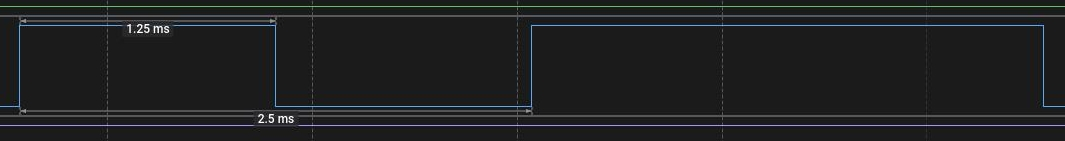
\includegraphics[width=0.7\textwidth]{../img/120rpm_to60_1.jpg}
  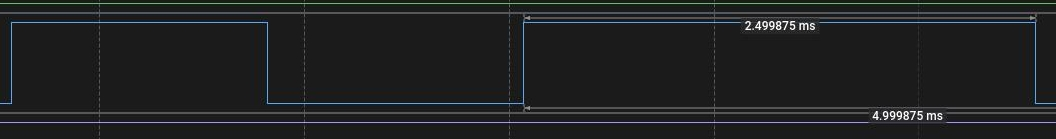
\includegraphics[width=0.7\textwidth]{../img/120rpm_to60_2.jpg}
  \caption[Moment of change between commands with 120RPM and 60RPM]{Moment of change between commands (120RPM $\Rightarrow$  60RPM)}
  \label{fig:switching}
\end{figure}

An attempt was made to also measure the delay  between switching commands, displayed in figure \ref{fig:switching}.
The results indicate that the delay between commands is imperceptible.
Similar outcomes were also observed for other command combinations.

This demonstrates the efficiency of the HAL layer in managing stepper motor control and transitioning seamlessly between commands.
As long as stepper queues are supplied with commands in advance, the platform can operate without noticeable interruptions.
Most importantly, the platform’s timely and predictable behavior ensures that mathematical corrections to the radar data can be applied accurately.



\chapter{Control application}

As previously stated control application for the whole system is written in MATLAB.
This application is split into two distinct parts - one is managing rotary platform and the other is processing radar data.
Alongside these there are some shared components, such as preferences menu.

\section{Main application interface}

Upon starting the application user is presented with the main window (Figure \ref{fig:main_window}).
This window is primarily used to display radar data and control basic functionality of the application.
On the sidebar user can enable serial connections to the radar and the platform, pause processing, save current visualization to jpg and in case of an emergency stop the platform.
Lastly topbar is used to access preferences and platform control interface.

\begin{figure}[h!]
  \centering
  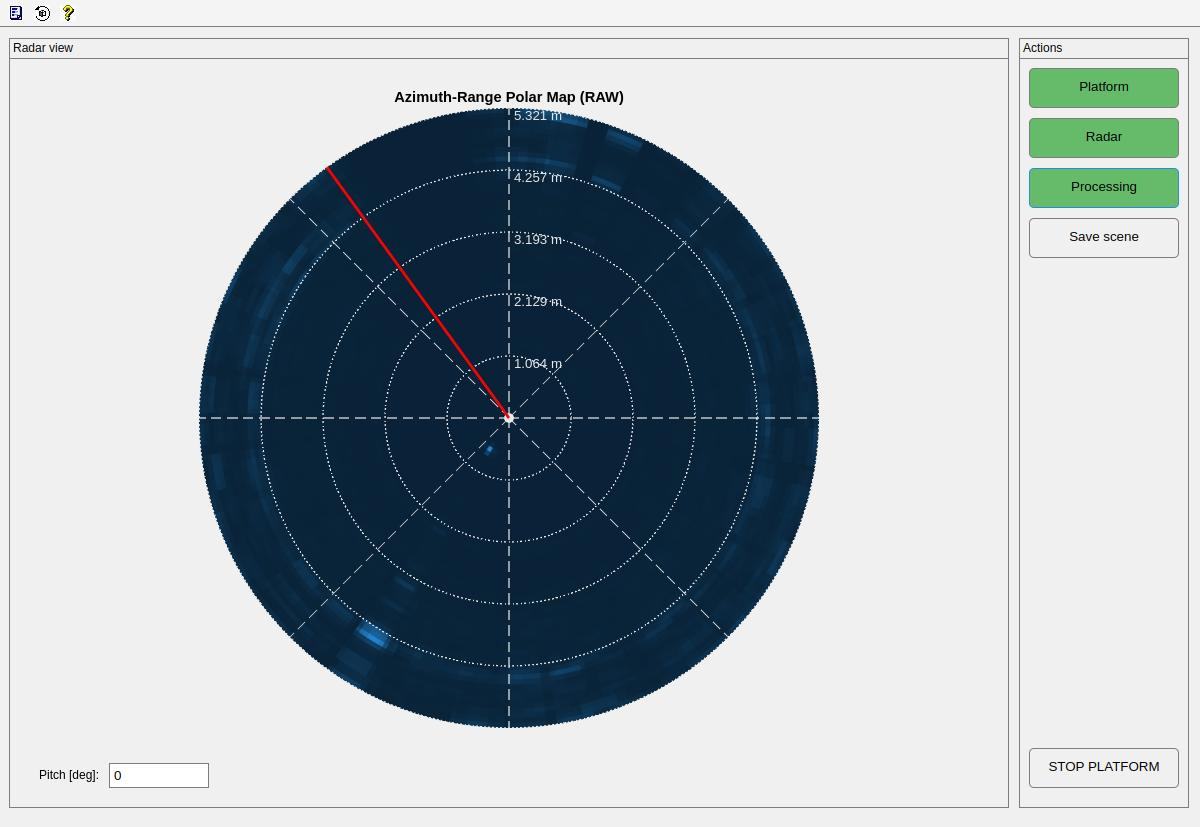
\includegraphics[width=0.9\textwidth]{../img/vis_range_azimuth.jpg}
  \caption[Main application window]{Main application window}
  \label{fig:main_window}
\end{figure}

\subsection{Configuration options}

As this thesis concerns itself with rather generic implementation of surveillance radar system the application is designed to be as flexible as possible.
For this purpose GUI menu was designed to enable configuration of all important elements - configuring the platform, radar, data processing and data visualization.
However it is necessary to point out that given extensive configuration options user is expected to have some knowledge about the subject to achieve satisfactory results in given application.
Firstly -- configuration options aren't checked againts each other if they aren't mutually exclusive.
For example speed calculation ramp averaging must be turned off, but this as things stand application will allow user to continue.
Secondly -- configuration of components such a CFAR or DBSCAN strongly depended on bandwidth, samples, NFFT and other parameters.
CFAR guard parameter of 3 might be too small on 5~GHz bandwidth where width of single range bin is only 50~mm, but if used on 24~GHz header with $BW=500$~MHz where range bin width is 50~cm it could be way too large.
To aid with choosing correct parameters the application provides some basic information like dimensions of the bins however it is up to the user to make the final decision.

Figure \ref{fig:preferences} shows the preferences menu, as one can see there are four main sections.
First configures serial port connections to the radar and the platform.
However baudrates are usually fixed  -- 230400 or 1000000 for the radar, depending on the firmware used and 115200 for the platform.
Second section handles configuration of the platform, followed by a section designated for radar configuration.
Last section configures how the data are processed and via which method they are visualized.

\begin{figure}[h!]
  \centering
  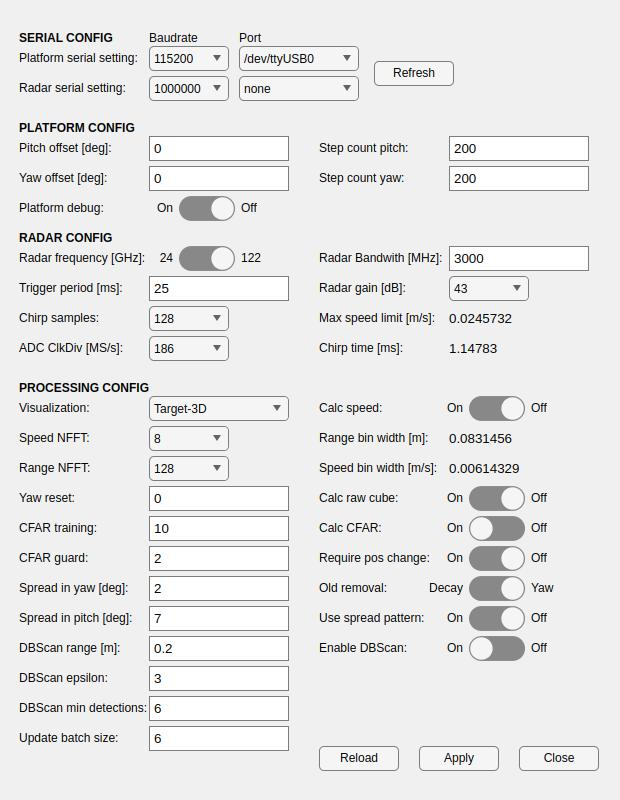
\includegraphics[width=0.7\textwidth]{../img/preferences.jpg}
  \caption[Preferences menu]{Preferences menu}
  \label{fig:preferences}
\end{figure}

User's preferences are stored in a INI file format in directory whose path depends on used operating system -- \texttt{\%APPDATA\%/Local/fmcw/fmcw.conf} on Windows and \texttt{\$HOME/.config/fmcw/fmcw.conf} for unix based systems.
As INI format is easily human readable and editable it is possible to edit the file directly.


\section{Platform Control Interface}

It is necessary to emphasizes that the platform control is entirely independent of the radar operation.
User loads up program to the platform, starts its execution and from then application is only processing current position reports comming from the platform.
There is no feedback from the radar to the platform based on processed data, although as the platform enables direct access to the stepper queues it would be possible to implement such a feature.
Nor does processing take into account from which movements is platform program comprised.

In preferences menu \ref{fig:preferences} user can configure static offsets to the platform with the \texttt{Pitch offset} and \texttt{Yaw offset} options.
This is useful in case zero positionof the platform is not aligned with what user want's to be zero in data.
Aside form offset step count configuration is also available here with \texttt{Step count pitch} and \texttt{Step count yaw}.
Step count takes into accoun both microstepping and physical down gearing ratio.
It is important to note that as platform doesn't store step count in non volatile memory this setting is essential to maintain propper operation of the platform.
The step count command is sent to the platform each time it is connected or config is changed.
Lastly \texttt{Platform debug} toggle enables full debug output to be visible in platform control window.

\begin{figure}[h!]
  \centering
  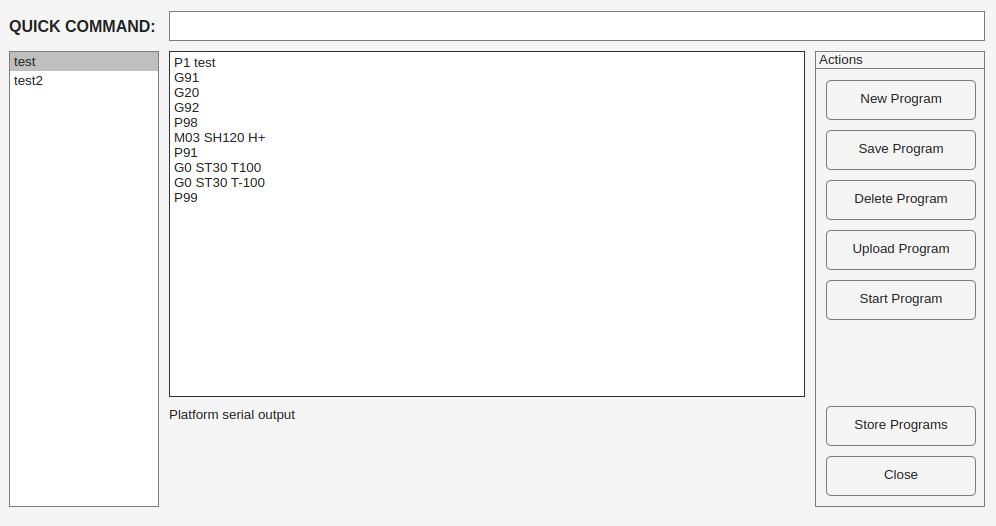
\includegraphics[width=\textwidth]{../img/platform_control.jpg}
  \caption[GUI of the platform control]{GUI of the platform control}
  \label{fig:platformControl}
\end{figure}

Managing platform programs is done via a separate window (Figure \ref{fig:platformControl}).
This interface allows user to load, edit and send programs to the platform.
Left sidebar allows user to load stored programs by clicking on their name.
Middle text boxes are used to edit programs header (top part) and program body (middle part) with bottom text field being used to display platforms debug output.
On the right side are then buttons that handle basic operations over program -- load, save, store to file, upload and start.

Commands are written one per line in G-code like syntax.
Control commands used to denote start of program, end of header and so on are automatically sent to the device when rest of the program is uploaded.
To validate whether program was parsed correctly user can consult the text window at the bottom of the screen which forwards platforms debug output to the user.
In case user clicks the store button the program is stored in same INI file as preferences.


Backend side of the platform control is rather straightforward.
After connection is established MATLAB serial interface calls a callback each time terminator sequence is found in received data.
Received message is then parsed with debug output being forwarded to the user and positions logged with timestamp in a circular buffer.
Radar data processing part can then request a list of positions for given time interval.

Platform control can also emit an event when platform finds itself close to a predetermined position.
This location is specified in option \texttt{Yaw reset} with tolerance zone fixed at two degress on either side.
In orde to prevent multiple emission of the event the platform will only emit it once per 1~s.
This event allows rest of the code to delete stored data and start gathering new one in next cycle.

\section{Radar configuration}

Given that the radar's output is displayed in the main window there isn't any specialized interface dedicated just to the radar.
Still in preferences menu (figure \ref{fig:preferences}) there are some paramters that can be configured.

\texttt{Radar frequency} toggle chooses between 24~GHz and 122~GHz header.
However this only affect configuration sent to the radar, it doesn't reflash the firmware what is also necessary to do.
After base frequency \texttt{Radar bandwidth} can also be configred, both positive and negative values are accepted however manual verification is required to verify that the radar is working as expected.
While manufacturer states a 3~GHz limit on the 24~GHz header and 5~GHz on the 122~GHz header \cite{sidarPRO}, in practice, especially with the 24~GHz header, achievable bandwidth was usually much lower.

User can also configure the number of samples per chirp via \texttt{Chirp samples} and ADC rate with \texttt{ADC ClkDiv}.
These two paramters determine time of a single ramp which is calcualted with equation \ref{eq:sampling}.
Together with gain, ramp time plays a crutial role in maintaining correct signal to noise ratio.

Drop down menu \texttt{Ramp coherent avg} allows user to pick how many ramps will be averaged together.
However use of this feature is generally not recommended unless surrounding environment is too cluttered (such as in a lab).
Each ramps adds some 2~ms overhead to the radar's operation and makes speed calculation impossible.


Last paramters is \texttt{Trigger period} which dictates how often will the application send a trigger command to the radar.
As previously stated the radar is at best capable of around 50~Hz update rate or 20~ms per chirp with slightly more stable performace at some 22~ms.


\chapter{Radar Data Processing}

Firstly it is necessary to outline what inputs and outputs of the whole processing pipeline are.
Data to the applications comes from two sources - serial connections to the radar and to the platform.
These two streams are then paired together based on timestamps logged when a data is received.
Processing than does user chosen calculations -- parts such as CFAR calculation, speed calculation and so on can be turned on or off.
Output data are then stored in radar cube, common method to manage radar's data that enables easy integration of more complex algorithms in the future \cite{richards2022}.

Given that both CFAR and raw data (That is individual range-Doppler maps.) calculation might need to be stored application has two cubes.
One is a 4D structure with dimensions of fast time $\times$ slow time $\times$ yaw $\times$ pitch, used to store complete range-Doppler map for each spatial degree.
In this thesis this structure is only used for visualizing of raw data for given fixed pitch angle or showing range-Doppler map for given yaw and pitch.
Any 3D visualization style of the raw data would be too cluttered and hard to interpret.
Second cube is a 3D structure with dimensions of range $\times$ yaw $\times$ pitch, this one is used to store CFAR output.

In each case yaw resolution is fixed 1 degree thus the cube is 360° wide.
Given quality of radar mounting bracket, 1.8° resolution of stepper and tighthness of radiation pattern 1° degree was deemed sufficient.
As for pitch same resolution was kept with angles rangeing form -20° to +80° being covered.
Lower bound is limited by the radar's mounting bracket and upper bound is more or less arbitrary, slightly guided by attempt to perevent radar from seeing behind itself.

Main complicating factor in the processing was the need to keep main thread responsive.
Most time critical thing main thread does is timely readout of data at serial ports.
If data can't be read right after its arrival assigned timestamps will be incorrect and visualization will be wrong.
In addition GUI starts to be quite unresponsive if the resources of main thread are stretched too thin.

To solve this problem processing heavily leverages MATLAB's parallel computing toolbox, offloading as much as possible to different cores.
Thorough whole processing pipeline there are mechanism of buffering data into larger batches and if needed discarding some in case software is unable to keep up.
Unfortunately as MATLAB's parallelization capabilities with threads are rather limited  -- external language interface don't work and so is the case for certain file/memory mapping functions \cite{matlabParallel}.
Thus the parallelization needs to be done with processes.
This restrict the application to machines with at least 16~GB of RAM as each process (of which there are three) requires around 2~GB of RAM.

Procesisng pipeline can be divided into multiple distinct steps as follow:
\setlist[enumerate]{nosep, topsep=3pt, partopsep=3pt}
\begin{enumerate}
  \item Data acquisition: Data are read, simple FFT is calculated and data are buffered into a circular buffer.
  \item Data processing: Data retrived from the  circular buffer paired with positions and processed.
  \item Cube update: Processed data are buffered into a ping-pong buffer. In case buffer is full the cube update routine is launched.
  \item Visualization: After cubes are updated data are visualized in user chosen format.
\end{enumerate}

\section{Data acquisition}

Basic workflow of this step is showned on figure \ref{fig:radar_flow}.
Action starts as soon as MATLAB detects line terminator within incoming data stream.
After whole frame from the radar is read, the data are timestamped and I and Q channels buffered.
Observer \texttt{dataProcessor.m} is then notified and left to  retrieves the data when main thread is free.


After retrieval inphase and quadrature channels are merged to for an complex singla which is multiplied by Hamming window.
Basic 1D FFT is then calculated with $NFFT$ equal to \texttt{Range NFFT}, in case fft order is larger than the number of samples zero padding is added.
Resulting spectrum is again buffered, as spectrums will be subjected to futher processing they are kept in original complex form.
Following this step program has multiple FFT spectrums computed -- those can be leveraged to enable range-Doppler map computation.

Program then verifies if the platform has moved.
This check enables to save processing resources by not computing R-D map that would be immediately rewritten.
After movement code than takes all spectrums (Except the last one when platform changed position.) and launches another processing step in a separate thread.
In case user wishes for procesisng to always take place (e.g. they are verifying radar settings when platform is static) this check can be skipped by toggeling \texttt{Require pos change}.



\begin{figure}[h!]
  \centering
  \begin{tikzpicture}[node distance=1.5cm, scale=0.6]

    % Layer headers
    \node (radar_header) [layerheader] at (0, 0) {radar.m};
    \node (processor_header) [layerheader] at (7.5, 0) {dataProcessor.m};

    % Radar Module
    \node (radar_start) [startstop, below of=radar_header, yshift=-0.3cm] {Start};
    \node (read_serial) [process, below of=radar_start] {Read serial data};
    \node (buffer_raw) [process, below of=read_serial] {Buffer raw data};
    \node (notify) [process, below of=buffer_raw] {Notify observers};

    % Data Processor Module
    \node (proc_start) [startstop, below of=processor_header, yshift=-0.3cm] {On notify};
    \node (read_radar) [process, below of=proc_start] {Read radar data};
    \node (calc_fft) [process, below of=read_radar, align=center] {Calculate FFT\\ Buffer spectrum};
    \node (check_pos) [decision, below of=calc_fft, yshift=-1cm, align=center] {Position\\ changed?};
    \node (get_spectrums) [process, right of=read_radar, xshift=4cm, align=center] {Get spectrums};
    \node (get_positions) [process, below of=get_spectrums] {Get positions};
    \node (cfar_process) [process, below of=get_positions, align=center] {Launch 2D/CFAR\\ processing};
    \node (proc_stop) [startstop, below of=check_pos, yshift=-1.3cm] {End};

    % Arrows for Radar Module
    \draw [arrow] (radar_start) -- (read_serial);
    \draw [arrow] (read_serial) -- (buffer_raw);
    \draw [arrow] (buffer_raw) -- (notify);
    \draw [arrow] (notify.west) -- ++(-1,0) |- (read_serial.west);
    %
    % % Arrows for Data Processor Module
    \draw [arrow] (proc_start) -- (read_radar);
    \draw [arrow] (read_radar) -- (calc_fft);
    \draw [arrow] (calc_fft) -- (check_pos);
    %
    % % Yes branch
    \draw [arrow] (check_pos.east) -- ++(1,0) node[right] {Yes} |- (get_spectrums.west);
    \draw [arrow] (get_spectrums) -- (get_positions);
    \draw [arrow] (get_positions) -- (cfar_process);
    %
    % % No branch
    \draw [arrow] (check_pos.south) -- node[right] {No} (proc_stop.north);

    % \draw [arrow] (cfar_process.south) -- ++(0,-1.7) -| (proc_stop.east);
    \draw [arrow] (cfar_process.south) |- (proc_stop.east);
  \end{tikzpicture}
  \caption{Processing flow - Data acquisition}
  \label{fig:radar_flow}
\end{figure}

\section{Data processing}

This parallel process takes calculated FFT spectrums and their accompanying positions and processes them into single range-Doppler map and CFAR array .
Basic outline of the processing flow is shown in figure \ref{fig:feature_flow}.

\begin{figure}[h!]
  \centering
  \begin{tikzpicture}[node distance=1cm, scale=0.5]
    % Main horizontal flow
    \node (processor_header) [layerheader] at (0, 0) {dataProcessor.m};
    \node (start) [startstop, below =of processor_header] {Thread start};
    \node (rcs) [process, right = of start] {Calculate RCS};
    \node (cfar_decision) [decision, below = of start] {CFAR?};
    \node (raw_decision) [decision, right=1cm of cfar_decision] {RAW?};
    \node (speed_decision) [decision, right=1.5cm of raw_decision] {Speed?};
    \node (return) [startstop, below=2.6cm of speed_decision] {Return};

    % CFAR branch
    \node (cfar_proc) [process, below=of cfar_decision, align=center] {Calc\\CFAR};


    % Speed branch
    \node (mock) [process, below left=1.5cm and -0.4cm of speed_decision, align=center] {Use last chirp\\ RCS array};
    \node (fft) [process, below right=1.5cm and -0.4cm of speed_decision, align=center] {2DFFT/\\NUFFT};

    % Connections
    \draw [arrow] (start.east) -- (rcs.west);
    \draw [arrow] (rcs.south) -- ++(0,-1) -| (cfar_decision.north);
    \draw [arrow] (cfar_decision.east) -- node[above] {No} (raw_decision.west);
    \draw [arrow] (cfar_decision.south) -- node[right] {Yes} (cfar_proc.north);
    \draw [arrow] (cfar_proc.east)  -- ++(0.3,0) |- (raw_decision.west);
    \draw [arrow] (raw_decision.south) -- ++(0,0) node[left] {No} |- (return.west);
    \draw [arrow] (raw_decision.east) -- node[above] {Yes} (speed_decision.west);
    \draw [arrow] (speed_decision.south) -- ++(0, -0.5) node[above, xshift=-1cm] {No} -| (mock.north);
    \draw [arrow] (speed_decision.east) -- ++(0, 0) node[above, xshift=+0.5cm] {Yes} -| (fft.north);
    \draw [arrow] (mock.south) -- ++(0,0) |- (return.west);
    \draw [arrow] (fft.south) -- ++(0,0) |- (return.east);

  \end{tikzpicture}
  \caption{Processing flow - Data processing}
  \label{fig:feature_flow}
\end{figure}

In the first step last spectrum is converted to values proportional to the radar cross section (RCS) of the target.
Starting with equation \ref{eq:radar_eq} we can see that the target's RCS is proportional to the received power divided by fourth power of the distance to the target.
Range can be calculated from manufacturer's equation \ref{eq:rangeBin} and power is proportional to the square of values reported from the radar.
Given that constants of the radar equation changed based on configuration calibration would be required in ordet to get real RCS values.
However this calibration is not supported and thus onwards when refering to RCS we will be refering to the values proportional to the RCS and not real RCS of the object.

After RCS conversion if \texttt{Calc CFAR} is enabled CFAR will be runned on latest chirp in the batch.
In this application simple 1D CA-CFAR from MATLAB's Phased Array System Toolbox is used which parametrized with two variables -- number of guard bins (Those are excluded from the average and are right next to bin we are testing.) and number of training bins (Those are used to calculate the average.) \cite{matlab_cfar}.
Both these paramters are configurable from preferences menu with \texttt{CFAR training} and \texttt{CFAR guard}.
As already stated, due wide varriation in bin widths for different bandwidth both paramters are left to be configured to the user.

If raw data calculation is enabled (Using \texttt{Calc raw cube} toggle.) the program takes one of two paths depending on whether speed calculation is toggled on or off with \texttt{Calc speed}.
In case speed calculation is disabled the program just returns half of the original spectrum converted to RCS.

When speed calculation is on program firstly cuts of samples that are too far away from position of the latest chirp.
After that timing of chirps is also analyzed choosing wheter NUFFT or 2DFFT transformation should be used.
Decision which transformation to use is based solely on the ratio of maximal deviation of the chirp intervals to the median of the chirp intervals -- if this ration is over 20~\% NUFFT is used.
For more accurate measurement more complex method should have been used but as the radar timing data is not very precise not to mention radar can track only very slow moving objects, this method was deemed sufficient.
For simmilar resasons no correction for the rotation of the platform is done and the threshold for distance isn't user configurable.
Output range-Doppler map is then shifted in order to get 2D array with \texttt{Range NFFT} $\times$ \texttt{Speed NFFT} number of elements with speed going from $-\frac{\text{Speed NFFT}}{2}\cdot w $ to  $\left(\frac{\text{Speed NFFT}}{2}-1\right)\cdot w $, where $w$ is speed bin widht calcualted with (\ref{eq:Doppler3}).


\section{Cube update}

Last step of processing pipeline handles updates of radar cubes.
Range-Doppler maps and CFAR data are firstly buffered in a ping-pong buffer -- where one is being used to update the cube while the other is being filled with new data.
Upon filling the buffer they switch roles and cube update routine is launched.

As matlab processes do not share same memory space by default in order not to have redundant copies of cube matlab's memory mapping is used.
Using function \texttt{memmapfile} the cube is mapped to a file on the disk which can be shared between two processes \cite{matlab_memory}.
This approach might lead to some performance degradation if the cube is too large and cannot be held in RAM but in testing it was found that for cubes of size 512MB (roughly cube for range-Doppler map of 256 $\times$ 16 ) the program was still able to keep up with the radar.


\begin{figure}[h!]
  \centering
  \begin{tikzpicture}[node distance=1cm, scale=0.5]
    % dataProcessor.m flow
    \node (processor_header) [layerheader] at (0, 0) {dataProcessor.m};
    \node (proc_event) [startstop, below=of processor_header, align=center] {Chirp processed};
    \node (add_buffer) [process, below=of proc_event] {Add to ping-pong buffer};
    \node (buffer_full) [decision, below=of add_buffer] {Buffer full?};
    \node (start_update) [process, below=of buffer_full] {Start cube update};
    \node (end_func) [startstop, below=of start_update] {End function};

    % radarDataCube.m flow
    \node (cube_header) [layerheader] at (9.5, 0) {radarDataCube.m};
    \node (cube_start) [startstop, below = of cube_header] {Update started};
    \node (keep_raw) [decision, below = of cube_start] {Keep RAW?};
    \node (use_spread) [decision, right=of keep_raw, align=center, xshift=+0.7cm] {Use spread\\pattern?};
    \node (direct_update) [process, below=of use_spread, align=center] {Update raw cube\\decay?};
    \node (create_subcube) [process, below=of direct_update] {Create subcube};
		\node (aggregate) [process, below =of create_subcube, align=center] {Aggregate updates};
		\node (aggregate2) [process, below =of aggregate, align=center] {Update raw cube\\decay?};
    \node (keep_cfar) [decision, below=2cm of keep_raw] {Keep CFAR?};
    \node (update_cfar) [process, below=of keep_cfar, align=center] {Update CFAR cube\\ decay?};
    \node (cube_return) [startstop, below= of update_cfar] {Return};

    % Connections
    \draw [arrow] (proc_event) -- (add_buffer);
    \draw [arrow] (add_buffer) -- (buffer_full);
    \draw [arrow] (buffer_full.south) -- node[right] {Yes} (start_update.north);
    \draw [arrow] (start_update.south) -- (end_func.north);
    \draw [arrow] (buffer_full.west) -- ++(-1.5,0) node[left] {No} |- (end_func.west);
    %
    \draw [arrow] (cube_header) -- (cube_start);
    \draw [arrow] (cube_start) -- (keep_raw);
    \draw [arrow] (keep_raw.east) -- node[above] {Yes} (use_spread.west);
    \draw [arrow] (keep_raw.south) -- node[right] {No} (keep_cfar.north);
    \draw [arrow] (use_spread.south) -- node[right] {No} (direct_update.north);
    \draw [arrow] (direct_update.west) -- ++(0,0) -| (keep_cfar.north);
    \draw [arrow] (use_spread.east) -- ++(1,0) node[above] {Yes} |- (create_subcube.east);
    \draw [arrow] (create_subcube) -- (aggregate);
    \draw [arrow] (aggregate) -- (aggregate2);
    \draw [arrow] (aggregate2.west) -| ++(-0.5,12.396 ) -| (keep_cfar.north);
    %
    \draw [arrow] (keep_cfar.west) -- ++(-1,0) node[above] {No} |- (cube_return.west);
    \draw [arrow] (keep_cfar.south) -- node[right] {Yes} (update_cfar.north);
    \draw [arrow] (update_cfar.south) -- (cube_return.north);
    %
  \end{tikzpicture}
  \caption{Processing flow - Cube update}
  \label{fig:cube_flow}
\end{figure}

Update routine for cubs contating either CFAR or raw data, are quite simmilar, in case spread pattern is disabled.
New data are just added to the cube to their respective positions where they replace old ones.
In case cube is set to decay whole cube is multiplied by decay factor that is derived from platforms speed of movement (The slower the platform moves the slower the decay).
Using this option will lead to output more visually resembling radar output of traditional analogue radar systems where most recent data were brighter than the older ones.
However user needs to keep in mind that color changes doesn't mean a change in RCS values at that position.
In addition this operation is rather computationally expensive and is the primary reason updates to the cube must be buffered.
Even on smaller cubes of around 256~MB this operations takes around 50~ms to complete on a laptop i7-10210U CPU.
If change of value would be undesirable behaviour decay can be turned off in the settings in favour of hard reset of the cube based on trigger on specified yaw position.

Enabling spread pattern leads to degradation of quality of the data in exchange for better visualization quality -- especially in range-azimuth visualization style.
Instead of adding new data just to one position in the cube the range-Doppler map is spread over a larger area with a aid of 2D matrix, containg a 2D Gaussian function.
As the data in series are usually close to each other in terms of position instead of directly adding these contributions to the full cube much smaller cube is created that covers only the area needed for the batch.
This enables significant speedup as smaller memory size enables better cacheing.
After each update is aggregated to the subcube the original cube is update in one go.

Due to lacking performance of MATLAB on author's machine some parts of the cube update routine were implemented in C++ with the aid of MATLAB's MEX interface.
This enabled the use of AVX2 x86 instruction set extension to speed up floating point operations.
Chiefly decaying of the cube exhibited roughly two fold perforace increase thanks to SIMD instructions.


\section{Visualization}

After cube update finishes program returns to the main thread and the data are visualized.
Other than graphical access to the data is not possible.
However the application offers a number of different visualization styles to suit the user's needs.

\begin{enumerate}
	\item Range-Azimuth: Polar plot with range on the radius and azimuth on the angle.
	\item Range-Doppler: Classical xy plot with range on x axis and Doppler on y axis, if speed is not calculated the y axis is replaced with RCS value.
	\item Target-3D: CFAR data are displayed in 3D cartesian space
\end{enumerate}

\subsection{Range-Azimuth}

This visualization style is used to display the data in polar plot for fixed pitch angle.
Which pitch angle is used is chosen via the small textbox at the bottom left corner of the screen.
The demonstration of Range-Azimuth map can be seen on figure \ref{fig:main_window}, which captures testing with 122~GHz header with rather large bandwidth of 5~GHz giving only some 3 meters of range.

As for the form of the data instead of calculation projection into horizontal plane the data are displayed in a conical projection.
That is no additional calculations are are and the cone we get by fixing the pitch angle is simply stretched to a circle.
To aid with orientation in a plot simple line markers are added to provide range and angle reference points.

It necessary to point out that as 24~Ghz header radiation pattern in pitch is rather large at relatively low angles the radar provides information about a larger area of the scene.
And if the user wishes using the spread patterns allows to range-azimuth map to include data even from different pitch angles.

\subsection{Range-Doppler}

Picking this visualization style from the preferences menu will display the data in a classical xy plot for a fixed yaw and pitch angle.
Just as with Range-Azimuth map both angles are configurable via the textboxes at the bottom of the screen.
In cases when speed calculation is disabled the y axis is replaced with RCS value.

Main purpose of this visualization style is to provide verification method for the radar data processing and setting.
As the devkit doesn't report much of a useful errors and its technical documentation is sometimes incorrect (e.g. in allowed bandwidth values) it is useful to have a way to verify that the radar is working correctly.

\begin{figure}[h!]
  \centering
  \begin{subfigure}[b]{0.45\textwidth}
    \centering
    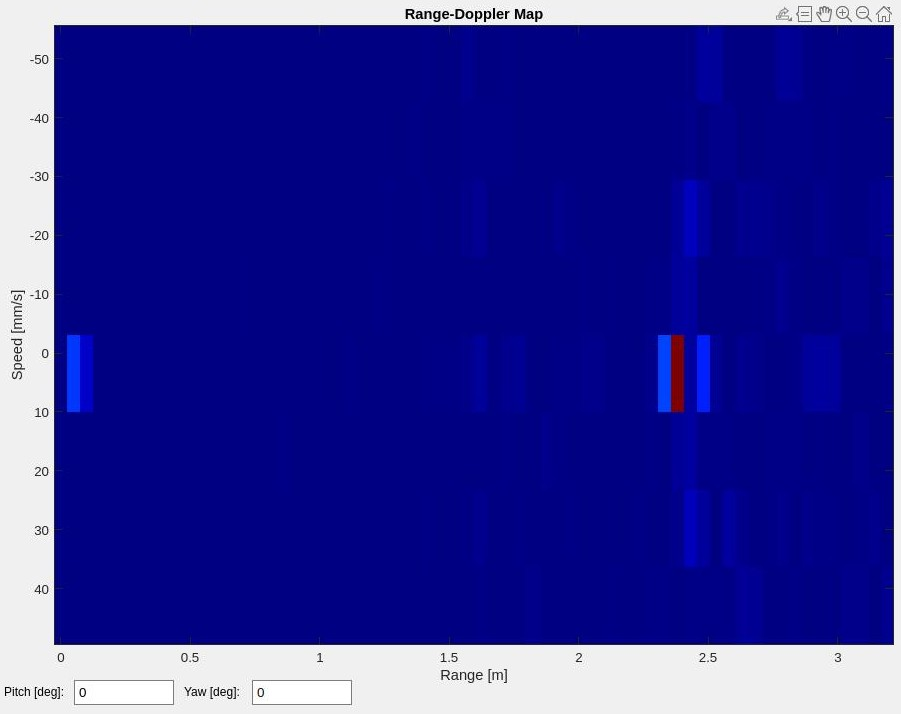
\includegraphics[width=\textwidth]{../img/vis_range_dop.jpg}
    \caption{Range-Doppler map}
  \end{subfigure}
  \hspace{0.05\textwidth}
  \begin{subfigure}[b]{0.45\textwidth}
    \centering
    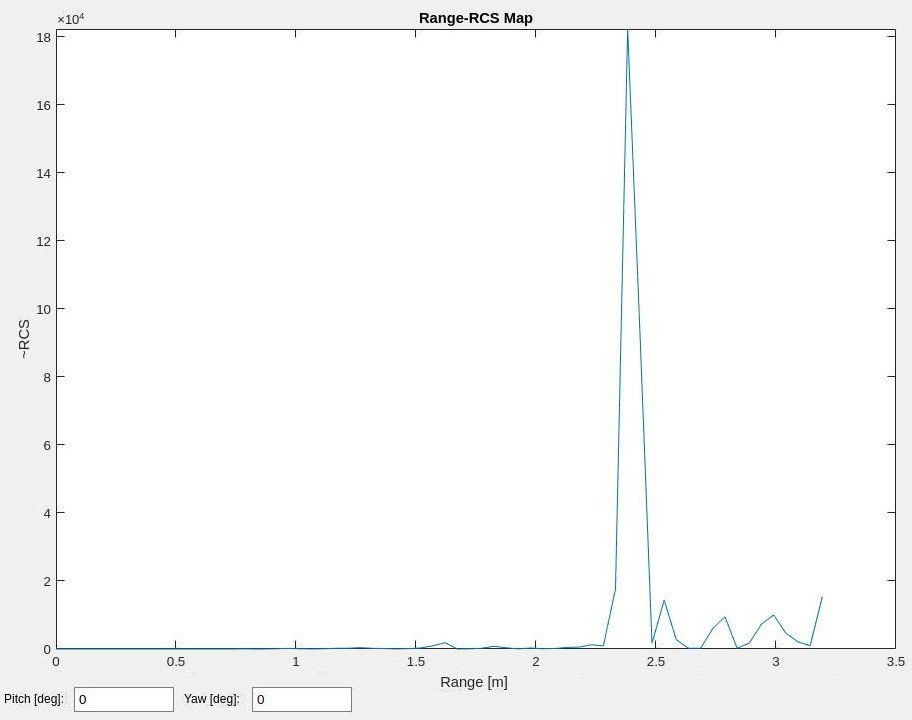
\includegraphics[width=\textwidth]{../img/vis_range_rcs.jpg}
    \caption{Range-RCS }
  \end{subfigure}
	\caption{Range-Doppler and Range-RCS maps}
  \label{fig:rd_rr_map}
\end{figure}

On figure \ref{fig:rd_rr_map} we can see two different visualization styles both displaying the same static scene.
As previously stated given rather poor sampling rate speed calculation is not very useful and thus no complex testing has taken.

\newpage
\subsection{Target-3D}

\begin{figure}[h!]
	\centering
	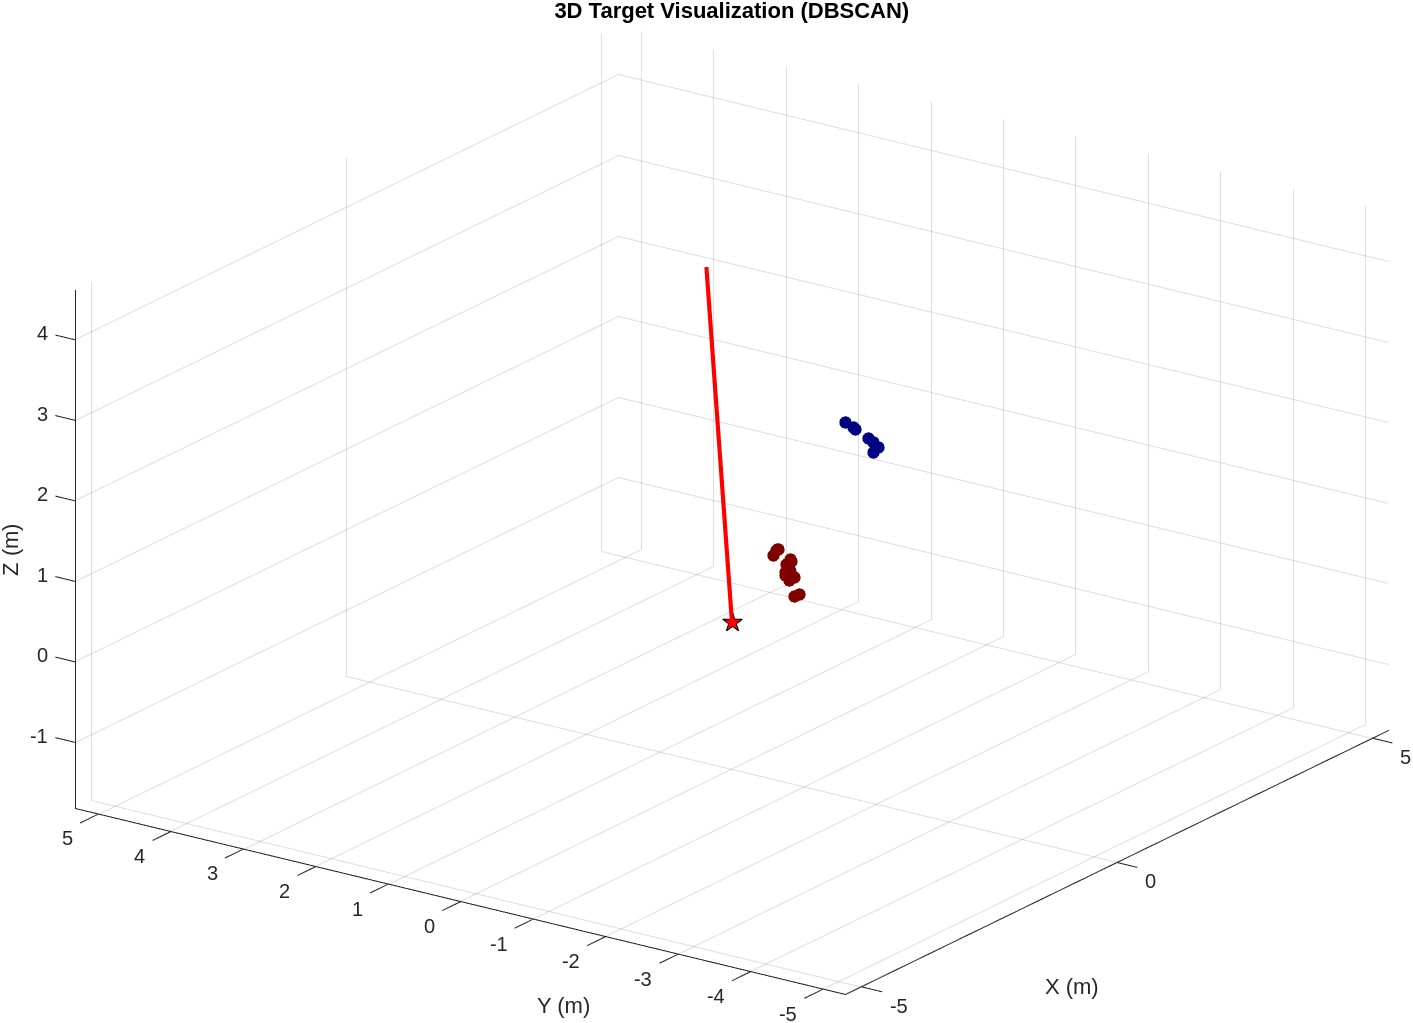
\includegraphics[width=0.9\textwidth]{../img/vis_3d.jpg}
	\caption[3D Space visualization method]{3D Space visualization method}
	\label{fig:vis3d}
\end{figure}

This visualization style is used to display CFAR data in 3D cartesian space (Figure \ref{fig:vis3d}).
Visualization method is rather simple with just positions being recalculated from the range, azimuth and pitch angles to x, y and z coordinates using trigonometric functions.
In case decay is enabled then small threshold is used to remove points whose values was sufficiently regraded.
To aid with orientation within the plot curret yaw and pitch of the platform at time of the update is also displayed as a red line;

If environment is too cluttered and CFAR generates too many points the user can enable basic clustering with matlab's built in DBSCAN function \cite{matlab_dbscan}.
Gerneral idea of DBSCAN is that to a given point in the dataset distances to other points are calculated and compared with user defined threshold $\varepsilon$, in case sufficient number $N$ of points is found within the threshold the point is marked as a cluster centers \cite{Kellner2012}.
In MATLAB's in algorithm distance threshold and minimal number of points are both configurable variables with other input being just the points list \cite{matlab_dbscan}.
As original data are in polar coordinates system problem arises with calculating distances given that in such system distance between two points of given fixed yaw and pitch varies widely with range.
Aside from that we also have significantly more points closer to the radar as space is much more densely scanned there compared to the far end of the range.
Both these factors lead to problems with choosing both $N$ and $\varepsilon$ paramters.

For accurate results these problems can be overcome using many different methods like using adaptive thresholds in relation to radius \cite{Kellner2012} or relying on more clever axis systems then just polar or cartesian \cite{Sun2024}.
However as in this thesis as DBSCAN is more of an illustration of possible postprocessing that can be added to existing base no such complex methods were implemented.
Both $\varepsilon$ and $N$ parameters are left to the user to configure.
Distance between points is the firstly converted to cartesian coordinates then metric is calculated using standard euclidean formula after which is later divided by average radius of the two points.
Still it needs to be said that, while dividing by the mean of distances is sometimes used when working with spherical data \cite{Fisher1993}, author is not aware of any literature that would suggest use in DBSCAN.
Especially on longer distance this methods will lead to significant errors.






% vim.ft=tex
\chapter*{Conclusion}
\addcontentsline{toc}{chapter}{Conclusion}

TODO


%%% Bibliography (literature used as a source)
%%%
%%% We employ biblatex to construct the bibliography. It processes
%%% citations in the text (e.g., the \cite{...} macro) and looks up
%%% relevant entries in the bibliography.bib file.
%%%
%%% See also biblatex settings in thesis.tex.

%%% Generate the bibliography. Beware that if you cited no works,
%%% the empty list will be omitted completely.

% We let bibliography items stick out of the right margin a little
\def\bibfont{\hfuzz=2pt}

\printbibliography[heading=bibintoc]

%%% If case you prefer to write the bibliography manually (without biblatex),
%%% you can use the following. Please follow the ISO 690 standard and
%%% citation conventions of your field of research.

% \begin{thebibliography}{99}
%
% \bibitem{lamport94}
%   {\sc Lamport,} Leslie.
%   \emph{\LaTeX: A Document Preparation System}.
%   2nd edition.
%   Massachusetts: Addison Wesley, 1994.
%   ISBN 0-201-52983-1.
%
% \end{thebibliography}


\listoffigures

\listoftables

\chapter*{Appendix}

\section*{Appendix A -- G-code glossary}

\setlist[itemize]{nosep, topsep=3pt, partopsep=3pt, leftmargin=*}
\setlist[description]{nosep, topsep=1pt, partopsep=1pt, leftmargin=*}

Following sections act as a glossary of all G-code commands used in the platform control. More in-depth descriptions of the commands can be found in the source code documentation.

\subsection*{Constants}

\begin{itemize}
  \item Parameters defined in Kconfig (require firmware recompilation):
  \item \texttt{STEPPER\_Y\_STEP\_COUNT}, \texttt{STEPPER\_P\_STEP\_COUNT}: Steps per rotation (modifiable via \texttt{M92}, non-persistent)
  \item \texttt{STEPPER\_[Y/P]\_PIN\_DIR}, \texttt{STEPPER\_[Y/P]\_PIN\_STEP}: GPIO pins for direction/step signals
  \item \texttt{STEPPER\_[Y/P]\_PIN\_ENDSTOP}: Endstop detection pins
  \item \texttt{STEPPER\_MAX\_SPEED}: Maximum RPM (hardware limit)
  \item \texttt{STEPPER\_DEFAULT\_SPEED}: Default motion RPM
  \item \texttt{STEPPER\_MIN\_SPINDLE\_TIME}: Minimum step interval of rotation in spindle mode
  \item \texttt{STEPPER\_HAL\_TIMER\_PERIOD/RESOLUTION}: PWM timer period/resolution, affects achievable RPM range
\end{itemize}

\subsection*{Features}

\begin{itemize}
  \item \textbf{Units}: Switch between degrees and steps using \texttt{G20}/\texttt{G21} respectively
  \item \textbf{Positioning Modes}:
    \begin{itemize}
      \item Absolute (\texttt{G90}): Automatically normalizes angles to [0, 360°] or [0, STEP\_COUNT]
      \item Relative (\texttt{G91}): Limited to $\pm$32767 steps per command, or respective angle counterpart
      \item in absolute positioning devices moves in the shortest path to the target
    \end{itemize}
  \item \textbf{Spindle}: Continuous rotation mode
  \item \textbf{Limits}: Limits on rotation can be imposed on both axes
    \begin{itemize}
      \item Limits are applied only to one rotation—it is not possible to restrict to, e.g., two full rotations in one direction and one in the other
      \item \texttt{low < high}: Valid range [low, high]
      \item \texttt{low > high}: Valid range [low, 360°] $\cup$ [0, high]
      \item Out-of-range targets snap to nearest valid position
    \end{itemize}
  \item \textbf{Programming}: G-code program can be uploaded to the device and executed
  \item \textbf{Synchronization}: If a command is issued to both axes, they will wait for each other; otherwise, the other axis will be free to execute the next command
\end{itemize}
\newpage

\subsection*{Motion Control Commands}

Axes are denoted as \texttt{Y} for yaw and \texttt{P} for pitch. The \texttt{S} parameter is used for speed for both axes, while \texttt{SY} and \texttt{SP} are used for the speed of yaw and pitch respectively. In the case of spindle, \texttt{Y} or \texttt{P} are not followed by step count/angle but instead by rotation direction.

\begin{description}
  \item[\texttt{M80}] Enable high-voltage power (enables drivers)
  \item[\texttt{M81}] Disable high-voltage power (disables drivers)
  \item[\texttt{M82}] Emergency stop (clears command queues)
  \item[\texttt{G20}] Set units to degrees
  \item[\texttt{G21}] Set units to steps
  \item[\texttt{G90 [Y/P]}] Set absolute positioning Mode
    \begin{itemize}
      \item Absolute positioning is not available in spindle mode; if you issue an M03 command to a stepper in absolute positioning mode, it will be automatically switched to relative positioning and throw an error
      \item If no argument is provided, both axes are switched to relative positioning
    \end{itemize}
  \item[\texttt{G91 [Y/P]}] Set relative positioning Mode
  \item[\texttt{G28 [Y/P]}] Auto-home specified axis(es)
  \item[\texttt{G92 [Y/P]}] Set current position as zero
  \item[\texttt{G0 Y<val> P<val> [SY/SP<rpm>]}] Stepper-mode movement
  \item[\texttt{M03 Y/P<+/-> [SY/SP<rpm>]}] Start spindle mode (continuous rotation)
  \item[\texttt{M05 [Y/P]}] Stop spindle mode
  \item[\texttt{M201 LY/HY/LP/HP<angle>}] Set angular limits (degrees/steps)
  \item[\texttt{M202 [Y/P]}] Disable limits
\end{description}

\subsection*{Special Commands}

These commands bypass certain sections and safety checks of the firmware. Use with caution.

\begin{description}
  \item[\texttt{G3 Y/P<steps> [SY/SP<rpm>]}] Bypass scheduler and adds movement directly to the queue
		\begin{itemize}
			\item Limits are not and cannot be checked
			\item Absolute positioning is not available
			\item All values are interpreted as steps regardless of current unit setting
			\item \textit{Warning}: Use \texttt{M82} before \texttt{G3} to maintain position integrity
		\end{itemize}
  \item[\texttt{W3 T<ms>}] Application-layer delay
		\begin{itemize}
			\item Useful to wait for end of homing process
		\end{itemize}
\end{description}

\subsection*{Programming Commands}
\begin{description}
  \item[\texttt{P90 <id>}] Start programming mode (overwrites existing program if any)
  \item[\texttt{P91}] Transition from header to main program body
  \item[\texttt{P92}] Finalize program (discarded if loops unclosed)
  \item[\texttt{P21 I<iterations>}] For-loop declaration
  \item[\texttt{P22}] End loop block
  \item[\texttt{P29}] Infinite loop marker (header only) - main body will be executed infinitely
  \item[\texttt{W0 Y/P<sec>}] Wait in seconds
  \item[\texttt{W1 Y/P<ms>}] Wait in milliseconds
\end{description}


\subsection*{Uplink Protocol}

\begin{itemize}
  \item \texttt{!P <timestamp>, <yaw>, <pitch>}: Position update (20ms interval)
  \item \texttt{!R OK}: Command acknowledgment
  \item \texttt{!R ERR <code>}: Command error
\end{itemize}

\begin{tabular}{ll}
  \hline
  \texttt{Code} & Description                          \\
  \hline
  1             & Malformed command syntax             \\
  2             & Invalid arguments                    \\
  3             & Queue lock failure                   \\
  4             & Unsupported command                  \\
  5             & System busy (homing/program running) \\
  6             & Runtime exception                    \\
  7             & Unclosed loop in program             \\
  8             & Invalid context                      \\
  \hline
\end{tabular}


\subsection*{Example Program}
\begin{tabular}{lll}
  \hline
  \texttt{Command}       & Mode   & Purpose                   \\
  \hline
  \texttt{P90 prog}      & Header & Initialize program ID=1   \\
  \texttt{G91}           & Header & Set relative positioning  \\
  \texttt{P29}           & Header & Enable infinite looping   \\
  \texttt{M03 SY6 Y+}    & Body   & Start Yaw spindle (6 RPM) \\
  \texttt{G0 SP30 P100}  & Body   & Pitch movement            \\
  \texttt{G0 SP30 P-100} & Body   & Return pitch              \\
  \texttt{P92}           & Body   & Finalize program          \\
  \hline
\end{tabular}


\clearpage
\openright
\end{document}
